%%%%%%%%%%%%%%%%%%%%%%%%%%%%%%%%%%%%%%%%%%%%%%%%%%%%%%%%%%%%%%%
%% OXFORD THESIS TEMPLATE

% Use this template to produce a standard thesis that meets the Oxford University requirements for DPhil submission
%
% Originally by Keith A. Gillow (gillow@maths.ox.ac.uk), 1997
% Modified by Sam Evans (sam@samuelevansresearch.org), 2007
% Modified by John McManigle (john@oxfordechoes.com), 2015
%
% This version Copyright (c) 2015-2017 John McManigle
%
% Broad permissions are granted to use, modify, and distribute this software
% as specified in the MIT License included in this distribution's LICENSE file.
%

% I've (John) tried to comment this file extensively, so read through it to see how to use the various options.  Remember
% that in LaTeX, any line starting with a % is NOT executed.  Several places below, you have a choice of which line to use
% out of multiple options (eg draft vs final, for PDF vs for binding, etc.)  When you pick one, add a % to the beginning of
% the lines you don't want.


%%%%% CHOOSE PAGE LAYOUT
% The most common choices should be below.  You can also do other things, like replacing "a4paper" with "letterpaper", etc.

% This one will format for two-sided binding (ie left and right pages have mirror margins; blank pages inserted where needed):
\documentclass[a4paper,twoside]{ociamthesis}
% This one will format for one-sided binding (ie left margin > right margin; no extra blank pages):
%\documentclass[a4paper]{ociamthesis}
% This one will format for PDF output (ie equal margins, no extra blank pages):
%\documentclass[a4paper,nobind]{ociamthesis} 



%%%%% SELECT YOUR DRAFT OPTIONS
% Three options going on here; use in any combination.  But remember to turn the first two off before
% generating a PDF to send to the printer!

% This adds a "DRAFT" footer to every normal page.  (The first page of each chapter is not a "normal" page.)
\fancyfoot[C]{\emph{DRAFT Printed on \today}}  

% This highlights (in blue) corrections marked with (for words) \mccorrect{blah} or (for whole
% paragraphs) \begin{mccorrection} . . . \end{mccorrection}.  This can be useful for sending a PDF of
% your corrected thesis to your examiners for review.  Turn it off, and the blue disappears.
\correctionstrue


%%%%% BIBLIOGRAPHY SETUP
% Note that your bibliography will require some tweaking depending on your department, preferred format, etc.
% The options included below are just very basic "sciencey" and "humanitiesey" options to get started.
% If you've not used LaTeX before, I recommend reading a little about biblatex/biber and getting started with it.
% If you're already a LaTeX pro and are used to natbib or something, modify as necessary.
% Either way, you'll have to choose and configure an appropriate bibliography format...

% The science-type option: numerical in-text citation with references in order of appearance.
\usepackage[
natbib=true, 
style=authoryear, 
sorting=none, 
backend=biber, 
doi=true, 
backref=true,  
url=false, 
maxcitenames=1,
giveninits=true,
uniquelist=minyear,
isbn=false]{biblatex}
\newcommand*{\bibtitle}{References}

\AtEveryBibitem{\clearfield{pmid}}
\AtEveryCitekey{\clearfield{pmid}}

\usepackage{float}

% The humanities-type option: author-year in-text citation with an alphabetical works cited.
%\usepackage[style=authoryear, sorting=nyt, backend=biber, maxcitenames=2, useprefix, doi=false, isbn=false]{biblatex}
%\newcommand*{\bibtitle}{Works Cited}

% This makes the bibliography left-aligned (not 'justified') and slightly smaller font.
\renewcommand*{\bibfont}{\raggedright\small}

% Change this to the name of your .bib file (usually exported from a citation manager like Zotero or EndNote).
\addbibresource{references.bib}


% Uncomment this if you want equation numbers per section (2.3.12), instead of per chapter (2.18):
%\numberwithin{equation}{subsection}



%%%%% THESIS / TITLE PAGE INFORMATION
% Everybody needs to complete the following:
\title{Delineation of Meiotic Gene\\ Expression in Male Mice}
\author{Daniel John Wells}
\college{Linacre College}

% Master's candidates who require the alternate title page (with candidate number and word count)
% must also un-comment and complete the following three lines:
%\masterssubmissiontrue
%\candidateno{933516}
%\wordcount{28,815}

% Uncomment the following line if your degree also includes exams (eg most masters):
%\renewcommand{\submittedtext}{Submitted in partial completion of the}
% Your full degree name.  (But remember that DPhils aren't "in" anything.  They're just DPhils.)
\degree{Doctor of Philosophy}
% Term and year of submission, or date if your board requires (eg most masters)
\degreedate{Michaelmas 2020}


%%%%% YOUR OWN PERSONAL MACROS
% This is a good place to dump your own LaTeX macros as they come up.

% To make text superscripts shortcuts
	\renewcommand{\th}{\textsuperscript{th}} % ex: I won 4\th place
	\newcommand{\nd}{\textsuperscript{nd}}
	\renewcommand{\st}{\textsuperscript{st}}
	\newcommand{\rd}{\textsuperscript{rd}}

\usepackage{textgreek}

%%%%% THE ACTUAL DOCUMENT STARTS HERE
\begin{document}



%%%%% CHOOSE YOUR LINE SPACING HERE
% This is the official option.  Use it for your submission copy and library copy:
\setlength{\textbaselineskip}{22pt plus2pt}
% This is closer spacing (about 1.5-spaced) that you might prefer for your personal copies:
%\setlength{\textbaselineskip}{18pt plus2pt minus1pt}

% You can set the spacing here for the roman-numbered pages (acknowledgements, table of contents, etc.)
\setlength{\frontmatterbaselineskip}{17pt plus1pt minus1pt}

% Leave this line alone; it gets things started for the real document.
\setlength{\baselineskip}{\textbaselineskip}


%%%%% CHOOSE YOUR SECTION NUMBERING DEPTH HERE
% You have two choices.  First, how far down are sections numbered?  (Below that, they're named but
% don't get numbers.)  Second, what level of section appears in the table of contents?  These don't have
% to match: you can have numbered sections that don't show up in the ToC, or unnumbered sections that
% do.  Throughout, 0 = chapter; 1 = section; 2 = subsection; 3 = subsubsection, 4 = paragraph...

% The level that gets a number:
\setcounter{secnumdepth}{2}
% The level that shows up in the ToC:
\setcounter{tocdepth}{2}


%%%%% ABSTRACT SEPARATE
% This is used to create the separate, one-page abstract that you are required to hand into the Exam
% Schools.  You can comment it out to generate a PDF for printing or whatnot.
\begin{abstractseparate}
	% "not normally exceeding 300 words"

% 1/2 sentences basic into comprehensible to any scientist
Meiosis is a specialised cell division producing the haploid gametes required for sexual reproduction.
A key function of this process is to generate genetic diversity through recombination and independent assortment of homologous chromosomes.
Delineation of gene expression during this process has been challenging due to the heterogeneity of testis tissue and the lack of faithful \textit{in vitro} models.

%The mechanisms of meiosis have important implications in the fertility, speciation, and evolution of all sexually reproducing organisms.

% One sentence summarying result, "here we show"
Here we jointly analyse a single-cell resolution transcriptomic dataset of over 20,000 cells from both wild type and mutant mice.
We use dimensionality reduction methods to infer latent components of variation that represent transcriptional programmes, mutant specific pathological processes, and technical effects.
This approach simultaneously soft clusters cells, infers corresponding groups of co-expressed marker genes, and imputes sparse, noisy gene expression.
We were also able to infer, \textit{de novo}, transcription factor binding motifs for each component, revealing a general switch at the meiotic divisions.
We facilitate access to this resource by providing an interactive website \href{http://www.testisatlas.ml}{testisatlas.ml}.

%We also infer, \textit{de novo}, transcription factor binding motifs likely to be driving the patterns of co-expression we observe.

The high-resolution delineation of gene expression during the spermatogenic programme provides high-resolution clues to the function of understudied genes.
One such gene, \textit{Zcwpw1}, is highly co-expressed with \textit{Prdm9}, and has domains capable of recognising the unique combination of histone marks that PRDM9 deposits (H3K4me3 and H3K36me3).
By using a human \textit{in vitro} system of \textit{Zcwpw1} co-transfection with either human or chimp \textit{Prdm9}, we show that PRDM9 causes the recruitment of ZCWPW1 to its binding sites.
This recruitment is stronger than for sites with H3K4me3 alone and is CpG dependent.

Male \textit{Zcwpw1\textsuperscript{-/-}} mice have completely normal double strand break positioning, but severe repair and synapsis defects leading to complete testicular azoospermia.
Although PRDM9's effect of DSB positioning remains intact, PRDM9's effect of aiding synapsis appears to be abolished, with persistent DMC1 signal - most dramatically at the most strongly PRDM9 bound hotspots.

% Two or three sentences explaining what the main result reveals in direct comparison to what was thought to be the case previously, or how the main result adds to previous knowledge


%One or two sentences to put the results into a more general context

%Our results demonstrate

% Two or three sentences to provide a broader perspective, readily comprehensible to a scientist in any discipline, may be included in the first paragraph if the editor considers that the accessibility of the paper is significantly enhanced by their inclusion

%We anticipate this expression atlas
 % Create an abstract.tex file in the 'text' folder for your abstract.
\end{abstractseparate}


% JEM: Pages are roman numbered from here, though page numbers are invisible until ToC.  This is in
% keeping with most typesetting conventions.
\begin{romanpages}

% Title page is created here
\maketitle

%%%%% DEDICATION -- If you'd like one, un-comment the following.
%\begin{dedication}
%This thesis is dedicated to\\
%someone\\
%for some special reason\\
%\end{dedication}

%%%%% ACKNOWLEDGEMENTS -- Nothing to do here except comment out if you don't want it.
\begin{acknowledgements}
 	
This thesis would not have been possible without the support of many people, a few of whom I have space to thank below.

\subsection*{Individual}

To my parents, for their immeasurable love and support.

To my supervisors, Jonathan Marchini and Simon Myers, for taking me on as a student, for providing guidance and feedback, for having the patience to afford me the independence of carving my own path, and for your infectious enthusiasm for science.

To my collaborators and colleagues, Min Jung and Don Conrad; Emmanuelle Bitoun; Anjali Hinch, Gang Zhang, Peter Donnelly and Ben Davies; for generously sharing data and ideas.

To my first rotation supervisor Benjamin Schuster-Böckler for guiding me in my initial foray into genomics.

To my advisors and examiners, Luke Jostins, Chris Holmes, and John Todd for their valuable advice and feedback on my work.

To Julian Knight and Isabel Schmidt, for supporting the Genomic Medicine and Statistics programme and community as well as their support and advice to me personally.

To my coursemates and officemates, for their comradeship and support.

\subsection*{Institutional}

To the Wellcome Trust for providing generous funding through the Genomic Medicine and Statistics programme (grant 109109/Z/15/Z).

To the Wellcome Center of Human Genetics and the Department of Statistics for providing office space and talks.

To Linacre College, for providing accommodation, dining, and fitness facilities.
\end{acknowledgements}

%%%%% ABSTRACT -- Nothing to do here except comment out if you don't want it.
\begin{abstract}
	% "not normally exceeding 300 words"

% 1/2 sentences basic into comprehensible to any scientist
Meiosis is a specialised cell division producing the haploid gametes required for sexual reproduction.
A key function of this process is to generate genetic diversity through recombination and independent assortment of homologous chromosomes.
Delineation of gene expression during this process has been challenging due to the heterogeneity of testis tissue and the lack of faithful \textit{in vitro} models.

%The mechanisms of meiosis have important implications in the fertility, speciation, and evolution of all sexually reproducing organisms.

% One sentence summarying result, "here we show"
Here we jointly analyse a single-cell resolution transcriptomic dataset of over 20,000 cells from both wild type and mutant mice.
We use dimensionality reduction methods to infer latent components of variation that represent transcriptional programmes, mutant specific pathological processes, and technical effects.
This approach simultaneously soft clusters cells, infers corresponding groups of co-expressed marker genes, and imputes sparse, noisy gene expression.
We were also able to infer, \textit{de novo}, transcription factor binding motifs for each component, revealing a general switch at the meiotic divisions.
We facilitate access to this resource by providing an interactive website \href{http://www.testisatlas.ml}{testisatlas.ml}.

%We also infer, \textit{de novo}, transcription factor binding motifs likely to be driving the patterns of co-expression we observe.

The high-resolution delineation of gene expression during the spermatogenic programme provides high-resolution clues to the function of understudied genes.
One such gene, \textit{Zcwpw1}, is highly co-expressed with \textit{Prdm9}, and has domains capable of recognising the unique combination of histone marks that PRDM9 deposits (H3K4me3 and H3K36me3).
By using a human \textit{in vitro} system of \textit{Zcwpw1} co-transfection with either human or chimp \textit{Prdm9}, we show that PRDM9 causes the recruitment of ZCWPW1 to its binding sites.
This recruitment is stronger than for sites with H3K4me3 alone and is CpG dependent.

Male \textit{Zcwpw1\textsuperscript{-/-}} mice have completely normal double strand break positioning, but severe repair and synapsis defects leading to complete testicular azoospermia.
Although PRDM9's effect of DSB positioning remains intact, PRDM9's effect of aiding synapsis appears to be abolished, with persistent DMC1 signal - most dramatically at the most strongly PRDM9 bound hotspots.

% Two or three sentences explaining what the main result reveals in direct comparison to what was thought to be the case previously, or how the main result adds to previous knowledge


%One or two sentences to put the results into a more general context

%Our results demonstrate

% Two or three sentences to provide a broader perspective, readily comprehensible to a scientist in any discipline, may be included in the first paragraph if the editor considers that the accessibility of the paper is significantly enhanced by their inclusion

%We anticipate this expression atlas

\end{abstract}

%%%%% MINI TABLES
% This lays the groundwork for per-chapter, mini tables of contents.  Comment the following line
% (and remove \minitoc from the chapter files) if you don't want this.  Un-comment either of the
% next two lines if you want a per-chapter list of figures or tables.
\dominitoc % include a mini table of contents
%\dominilof  % include a mini list of figures
%\dominilot  % include a mini list of tables

% This aligns the bottom of the text of each page.  It generally makes things look better.
\flushbottom

% This is where the whole-document ToC appears:
\tableofcontents

\listoffigures
	\mtcaddchapter
% \mtcaddchapter is needed when adding a non-chapter (but chapter-like) entity to avoid confusing minitoc

% Uncomment to generate a list of tables:
%\listoftables
%	\mtcaddchapter

%%%%% LIST OF ABBREVIATIONS
% This example includes a list of abbreviations.  Look at text/abbreviations.tex to see how that file is
% formatted.  The template can handle any kind of list though, so this might be a good place for a
% glossary, etc.
% First parameter can be changed eg to "Glossary" or something.
% Second parameter is the max length of bold terms.
\begin{mclistof}{List of Abbreviations}{3.2cm}

\item[AUC] Area Under the Curve

\item[ChIP] Chromatin Immuno-precipitation

\item[CI] Confidence Interval

\item[CpG] Cytosine phosphodiester Guanine

\item[DSB] Double Strand Break

\item[dHJ] Double Holiday Junction

\item[DGE] Digital Gene Expression (count matrix)

\item[E10.5] Embryonic Day 10.5

\item[FACS] Fluorescence Activated Cell Sorting

\item[FET] Fishers Exact Test

\item[FISH] Fluorescent In Situ Hybridisation

\item[GAM] Generalised Additive Model

\item[GO] Gene Ontology

\item[GWAS] Genome Wide Association Study

\item[H3K4me3] Histone 3 Lysine 4 tri-methylation

\item[Het] Heterozygous

\item[Hom] Homozygous

\item[ICA] Independent Component Analysis

\item[KO] Knock Out

\item[MCA] Mouse Cell Atlas

\item[MSCI] Meiotic Sex Chromosome Inactivation

\item[mRNA] messenger Ribose Nucleic Acid

\item[NNMF/NMF] Non-Negative Matrix Factorisation

\item[NGS] Next Generation Sequencing

\item[OR] Odds Ratio

\item[PCA] Principal Component Analysis

\item[PCR] Polymerase Chain Reaction

\item[PIP] Posterior Inclusion Probability

\item[PND5] Post Natal day 5

\item[QC] Quality Control

\item[RT] Reverse Transcription

\item[SDA] Sparse Decomposition of Arrays

\item[scRNAseq] Single Cell RNA sequencing

\item[SNP] Single Nucleotide Polymorphism

\item[SPCI] Primary Spermatocyte

\item[SPCII] Secondary Spermatocyte

\item[SPG] Spermatogonia

\item[SPD] Spermatid

\item[SSDS] Single Stranded DNA Sequencing

\item[TF] Transcription Factor

\item[TFBS] Transcription Factor Binding Site

\item[TSS] Transcription Start Site

\item[t-SNE] t-distributed Stochastic Neighbourhood Embedding

\item[UMAP] Uniform Manifold Projection

\item[UMI] Unique Molecular Identifier

\item[UTR] Untranslated Region

\item[WT] Wild Type

\end{mclistof} 


% The Roman pages, like the Roman Empire, must come to its inevitable close.
\end{romanpages}


%%%%% CHAPTERS
% Add or remove any chapters you'd like here, by file name (excluding '.tex'):
\flushbottom
\begin{savequote}[8cm]
\textit{Es müsse eine Art der Kerntheilung geben, durch welche die im Mutterkern enthaltenen Ahnenplasmen dergestalt auf die Tochterkerne vertheilt werden, dass jedem Tochterkern nur die halbe Zahl derselben zukomme.}

There must be a form of nuclear division in which the ancestral germ plasms contained in the nucleus are distributed to the daughter nuclei in such a way that each of them receives only half the number contained in the original nucleus.
  \qauthor{--- \cite{Weismann1887Ueber}}
\end{savequote}

\chapter{\label{ch:1-intro}Background}

\minitoc


\section{Aims}
Meiosis is a type of cell division in which the number of chromosomes is reduced by half to produce haploid gametes (sperm and egg cells)~\parencite{Ohkura2015Meiosis}.
The primary aim of this research was to delineate the gene expression programme of spermatogenesis (during which meiosis occurs).
Specifically, to identify which genes are expressed, in which cells, their degree of expression, and relative timing during spermatogenesis.
With this atlas of expression data, we additionally aimed to infer the regulatory network controlling these expression patterns, as well as to predict protein function and in doing so identify targets for further characterisation.
Finally, we aimed to carry out such characterisation for at least one of these targets.


\section{Motivations}

%\subsection{Sexual Reproduction}
Reproduction is a fundamental property of all known life.
Of the three domains of life Eukaryotes/Eukarya are able to reproduce sexually, and almost all do.
The dominance of this trait has been estimated at roughly 99.9\% \parencite{White1978Modes}.
Although many Eukaryotes are able to reproduce asexually, those which do so exclusively are typically confined to the youngest branches of life, an often cited exception being the Bdelloid rotifers - although there is now evidence of rare sexual reproduction in this species \parencite{Debortoli2016Genetic, Laine2020Sexual}.
This shared characteristic was likely present in the common ancestor of this empire and hence synapomorphic \parencite{Bernstein2013Evolutionary}.
The sexual life cycle consists of an alternating halving of the genetic material/ploidy (by meiosis) to form haploid cells, followed by karyogamy (nuclear fusion).
Meiosis (from Ancient Greek, meíōsis, “a lessening”) is a specialised form of cell division, in which genetic material is exchanged between the parental genomes (recombination).
Recombination and independent assortment of homologous chromosomes generate genetic diversity and hence enable natural selection and evolution.
Recombination also ensures balanced segregation at the reductional division which follows (no naturally occurring eukaryotes have a single chromosome - although synthetic yeast has been engineered - \cite{Shao2018Creating}).

The mechanisms of meiosis have important consequences for the evolution, fertility, and speciation of sexually reproducing organisms~\parencite{Davies2016Reengineering,Hassold2007Origin}. 


%\subsection{Disease}
As the process of gamete generation, errors in meiosis can cause genetic disease in offspring.
In some sense the most extreme version is complete infertility, affecting around 10\% of humans (with many being of unexplained cause) \parencite{Datta2016Prevalence, Hamada2011Unexplained}.
Other errors can be compatible with fertilisation but not full gestation resulting in miscarriage (affecting around 13\% of pregnancies overall, but over 50\% for mothers over the age of 45 years - \cite{Magnus2019Role}).
Others errors are compatible with birth but result in incurable disease such as some aneuploidies \parencite{Hassold2007Origin} and microdeletion syndromes caused by non-allelic homologous recombination \parencite{Myers2008common}.


A better understanding of the mechanisms of spermatogenesis and meiosis could aid in the prevention of such diseases.
Additionally, determining the factors required for \emph{in vitro} spermatogenesis could enable the treatment of male infertility in addition to facilitating further research \parencite{Zhou2016Complete}.

While enabling the production of healthy offspring is one aim of reproductive medicine, \emph{preventing} fertilisation (usually but not always, temporarily) is also extremely important for the health of both mother and child \parencite{Cleland2012Contraception}.
Hence the development of contraceptives is another key goal of reproductive science, and one which a clearer delineation of testis specific genes could aid \parencite{Schultz2003multitude}.


%\subsection{Curiosity}
As with many scientific endeavours, curiosity is also a major driver of this research.
The testis is a most unusual tissue especially at the transcriptional level.
The testis has the highest number of tissue enriched genes out of the 32 tissues profiled in the Human Protein Atlas ($>$ five-fold higher mRNA levels in one particular tissue as compared to any other), with 1,057 enriched genes out of a total 2,489 across the 32 tissues~\parencite{Djureinovic2014human,Mele2015Human, Uhlen2015Tissuebased, Uhlen2016Transcriptomics, TheHumanProteinAtlas2019human}.
This is over twice as many as the second highest tissue the cerebral cortex which is perhaps considered the most complex tissue functionally, and with which the testis shares a surprising similarity \parencite{Guo2005Transcriptomic, Djureinovic2014human, Uhlen2015Tissuebased}.
More recent studies using single-cell sequencing have underscored the distinct transcriptional state of the testis (\cite{Han2018Mapping} and figure \ref{fig:MCA_PCA}).
The testis is also one of a few immune privileged sites in the human body \parencite{Fijak2006testis}.


\begin{figure}[H]
	\centering
	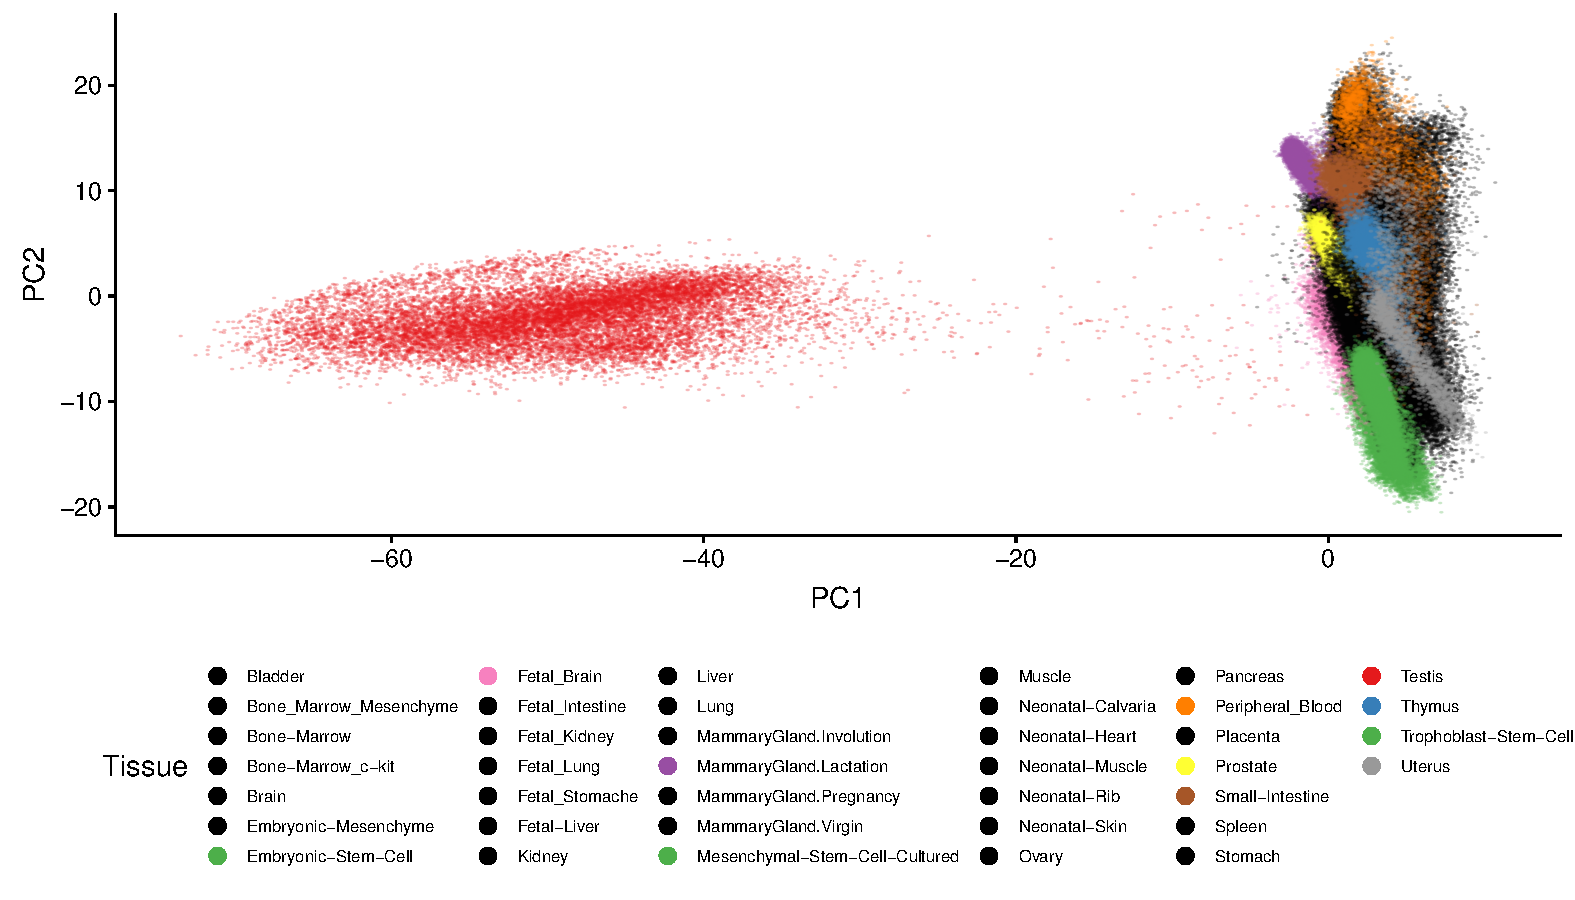
\includegraphics[width=\textwidth]{figures/intro/MCA_PCA.pdf}
	\caption[Testis PCA (MCA)]{PCA of single cell RNAseq of 50 different tissues and cell types from over 400,000 cells from the mouse. Data from~\cite{Han2018Mapping}}
	\label{fig:MCA_PCA}
\end{figure}


 The previous two properties have lead to the use of testis expressed genes as targets for cancer immunotherapy (cancer testis antigens) as when re-expressed in cancers they provide a distinguishing biomarker \parencite{Whitehurst2014Cause}.

Chromatin undergoes massive remodelling during spermatogenesis ultimately resulting in most (90/99\% in human/mouse) of the histones being replaced by crosslinked protamines, leading to the cessation of transcription \parencite{Rathke2014Chromatin}.
This necessitates long term mRNA storage ($>$5 days) before translation \parencite{Kleene2013Connecting}.

Sperm are a highly specialised cell, despite being a single cell and unable to transcribe new mRNA they must perform many of the functions of the whole organism including motility, sensing the environment (chemotaxis), and defence from attack (from the female immune system) \parencite{Kaupp2008Mechanisms, Thompson1992Leukocytic}.
Indeed they are able to survive and even fertilise after more than three days in the female reproductive tract \parencite{Gould1984Assessment,Wilcox1995Timing}.

Meiosis itself of course is also unique, with paternal and maternal homologous chromosomes being relatively unaware of each other in somatic cells, until pairing in meiosis in the germline.
In addition, it has been repeatedly observed that the majority (\textasciitilde80\%) of inherited single nucleotide mutations first arise in the testis \parencite{Kong2012Rate, Michaelson2012WholeGenome, Goldmann2016Parentoforiginspecific, Rahbari2016Timing, Jonsson2017Parental}.

%Incomplete cytokinesis


\subsection{Generating Maps of Gene Expression}
Much of science can be characterised as the creation of maps.
The discovery, description and cataloguing of various types of elements, which is often dismissed as `merely descriptive', is a fundamental bedrock of many sciences \parencite{Grimaldi2007Why}.
Maps are often useful in two senses, they serve as a reference of what's already known, but they also arrange current knowledge in such a way as to provide a prediction of the unknown.
For example Mendeleev's periodic table both catalogued the known elements but left gaps for new discoveries.
Equally with the Standard Model in physics.
Darwin and others made extensive catalogues of past and present diversity of life, eventually resulting in the concept of evolution by natural selection.
Cataloguing the ratios of offspring phenotypes lead to Mendel's laws.

Our maps of protein function are woefully incomplete, with more than 3,000 (15\%) of human genes not even having a biological process annotation (and a similar \% in the more experimentally amenable organisms \textit{S. cerevisiae} and \textit{S. pombe}) \parencite{Wood2019Hidden}.
Even genes with at least one annotation or paper are often incompletely or even incorrectly characterised.
Significant bias exists against initiating research into a gene of unknown function \parencite{Edwards2011Too, Stoeger2018Largescale, Haynes2018Gene}.
This can be partially attributed to risk averse incentives in scientific funding and evaluation.
In addition, for many proteins of unknown function there are limited tools available such as antibodies, making even simple characterisation difficult (for example immunofluorescence or immuno-precipitation based assays).


%\subsection{Maps of Protein Function}
Genome sequencing projects have provided single base resolution maps of many organisms' genomes (thousands of eukaryotes - \cite{Genome}).
This relatively unbiased approach has uncovered many genes of unknown function and has accelerated their characterisation.
For example, by enabling the inference of molecular function from homology with known domains, and by facilitating sequence based detection and cloning.
Ultimately much of what we care about is at the level of a phenotype such as infertility, and GWA studies provide one way to potentially associate genes with such phenotypes \parencite{Gajbhiye2018Complex}.
However, even \emph{if} a causal gene can be confidently identified for an associated SNP, because the phenotypes are usually broad, this often tells us little about the molecular function of a gene, necessitating substantial follow up research which is frequently not practical or undertaken \parencite{Visscher201710, Gallagher2018PostGWAS, Struck2018impact}.

In a reverse genetics approach, specific mutations are created and the phenotypic results are investigated.
The International Mouse Phenotyping Consortium aims to generate and broadly phenotype knockout mice for every protein coding gene, with a current catalogue of over 5,000 null mice models \parencite{2004Knockout,Meehan2017Disease, Birling2019resource}.

Other atlases such as the Human Protein Atlas and GTEx instead start from the first step in a gene's function, providing transcriptomic data enabling association of co-expressed genes and association of tissue specific genes with the function of those tissues.
However, bulk tissues are too heterogeneous and large scale to provide precise insights into molecular function.
Through a similar argument, proteins with co-varying abundances and protein-protein interactions can also implicate functions.

A protein's structure is often more conserved than its sequence and can give direct mechanistic insight into its function \parencite{Illergard2009Structure, Sousounis2012Conservation}.
Despite being less able to take advantage of advances in high throughput next generation sequencing technology, over 144,000 structures are held by the Protein Data Bank, many deposited by structural genomics programs, but still many protein families lack a single structure \parencite{wwPDBconsortium2019Protein, Grabowski2016Impact, Khafizov2014Trends}.

Recently, droplet based single cell RNAseq technologies have enabled higher resolution high-throughput characterisation of gene co-transcription.
A number of mapping projects have been launched including the Human Cell Atlas and Mouse Cell Atlas as well as other tissue specific maps including the one we present here, helping to provide much higher resolution clues for the function of unstudied genes \parencite{Regev2017Human,Regev2018Human,Han2018Mapping,TheTabulaMurisConsortium2018Singlecell}.
We will show that this allows us to more reliably associate particular groups of genes with specific functions, at specific times, in meiosis.


%%%%%%%%%%%%%%%%%%%%%%%%%%%%%%%%%%%%%%%%%%%%%%%%%%%%%%%%%%%%%%%%%%%%%%%%
\section{Measuring Gene Expression}
%%%%%%%%%%%%%%%%%%%%%%%%%%%%%%%%%%%%%%%%%%%%%%%%%%%%%%%%%%%%%%%%%%%%%%%%

Expression is the process through which information contained within the genome manifests as a phenotype.
This involves generation of a functional biomolecule, such as proteins but sometimes RNA (most importantly the ribosome).
The first step in expression is the generation of messenger(m) RNA and there are a number of different technologies available to quantify the amount of mRNA - each providing different types and amounts of information.

Physical limits make it challenging to sensitively and accurately quantify gene expression.
mRNA is <5\% of total RNA in a cell, with the rest comprising of ribosomal and transfer RNA \parencite{Warner1999economics}.
Total RNA content per eukaryotic cell is approximately 20pg, with <1pg of mRNA, corresponding to roughly <500,000 mRNA molecules \parencite{Roozemond1976Ultramicrochemical, Uemura1980Agerelated, Tang2011Development}.
Most genes have mRNA copy numbers of 1-100 per cell, up to a maximum of perhaps 1,000 \parencite{Marguerat2012Quantitative, Macaulay2014Single}.
At the level of individual cells, mRNA synthesis is ``bursty'' introducing further biological heterogeneity in expression measurements \parencite{Raj2006Stochastic, Chubb2006Transcriptional}.

\subsection{In Situ Hybridization}
In Situ Hybridisation, first described by \cite{Gall1969Formation}, uses a probe (either RNA or DNA) which is incubated with fixed cells and binds to a target mRNA by complementary binding and can then be visualised.
This has the advantage of being single cell resolution, and even allowing subcellular localisation to be observed.

Visualisation of the probe initially used radioactive labelling which was low resolution, expensive, unstable, and dangerous.
However, this was overcome by using biotinylated probes coupled with secondary detection \parencite{Singer1982Actin} and later directly fluorescent probes (FISH) \parencite{Kislauskis1993Isoformspecific}.

This sensitivity of this technique has been further increased by using multiple probes per target RNA, enabling the detection of individual mRNA molecules (single molecule smFISH - \cite{Femino1998Visualization, Raj2008Imaging}).
In addition, multiplexed detection schemes using multiple cycles of sequential hybridization and imaging such as SeqFISH(+) \parencite{Lubeck2014Singlecell,Eng2017Profiling,Eng2019Transcriptomescale} and MERFISH \parencite{Chen2015Spatially, Moffitt2016Highthroughput, Moffitt2016Highperformance, Xia2019Multiplexed} are able to measure many (up to 10,000) RNA targets.
These methods have the advantage that amplification is not necessarily required and the high sensitivity allows single molecules to be detected.
Furthermore, by measuring nuclear vs cytoplasmic localisation or by using probes to introns, mRNA dynamics (``RNA velocity'') and isoform usage can also be measured \parencite{Shah2018Dynamics, Xia2019Spatial}.

%(barcodes??)

\subsection{RT-qPCR}
Reverse transcription quantitative real-time PCR measures PCR products during the amplification by using fluorescent detectors \parencite{Gibson1996novel, Heid1996Real, Chiang1996Use}.
This technique is able to detect a single mRNA molecule, and has become the gold standard in expression quantification.
However, primers must be designed for each gene and any spatial information is lost \parencite{Palmer2003New, Wong2005Realtime}.

Furthermore, due to the exponential amplification, small differences in reverse transcription, primer efficiency, or initial starting amounts and contamination can lead to inaccurate quantification.
Therefore, efficiency and validated reference genes must be established by separate experiments \parencite{Bustin2009MIQE}.

\subsection{Northern Blot}
The Northern blot is one of the earliest methods for measuring mRNA levels \parencite{Alwine1977Method}.
It consists of RNA extraction, separation by gel electrophoresis, followed by transfer by blotting onto a membrane and finally detection by complementary hybridisation with a radioactive/fluorescent probe.
Northern blotting still remains a useful technique when information about the relative sizes of transcripts is required.

\subsection{Microarrays}
A microarray is typically a glass slide coated with cDNA oligomers.
mRNA with polyA tails can be extracted from total RNA using oligo(dT) beads, reverse transcribed to cDNA, fluorescently labelled, and washed over the array \parencite{Schena1995Quantitative, DeRisi1996Use, Schulze2001Navigating}.
The fluorescent intensity is a measure of the abundance of mRNA in the sample.
This approach allowed whole transcriptome quantification and was wildly popular, with the EBI ArrayExpress database passing 100,000 hybridisations in 2008 \parencite{Rustici2008Data}.

\subsection{Bulk RNA Sequencing}
The reducing cost rapidly led to the use of DNA sequencing technology to quantify the transcriptome \parencite{Mortazavi2008Mapping, Cloonan2008Stem, Wilhelm2008Dynamic, Lister2008Highly, Nagalakshmi2008Transcriptional}.
mRNA is extracted as for microarrays, fragmented, and sequenced using short read NGS technology before being re-mapped to the genome.
This has the advantage over microarrays that the sequence of hybridisation probes does not need to be designed from an already known transcriptome reference, enabling, for example, novel transcripts and splice isoforms to be discovered.
RNAseq provides a digital read out, in comparison to the analogue signal from microarrays which limited its replicability across platforms.
In addition, the dynamic range is much greater than for microarrays in which the signal saturates when all probes are bound and at low concentrations non-binding is favoured \parencite{Zhao2014Comparison}.
RNAseq also enables detection of sequence variants and allele specific expression.
For these reasons RNAseq has become the standard method for profiling the transcriptome \parencite{Stark2019RNA}.

As it is based on standard sequencing technology RNAseq, benefits from advances in next generation sequencing.
For example, long read technology from PacBio enables full transcript (cDNA) sequencing - enabling the unambiguous identification of transcript isoforms which previously had to be inferred using the fragmentation approach of short read sequencing \parencite{Sharon2013singlemolecule, Cartolano2016cDNA}.
Oxford Nanopore sequencing infers the sequence of polynucleotides from the change in current as they pass through a nanopore embedded within a membrane across a voltage.
In addition to being able to sequence long reads as PacBio \parencite{Oikonomopoulos2016Benchmarking}, this technology was recently demonstrated to be able to sequence mRNA directly, bypassing the fragmentation, reverse transcription, PCR amplification and size selection steps, reducing opportunities for bias \parencite{Garalde2018Highly, Workman2019Nanopore}.
Furthermore Oxford Nanopore sequencing is able to quantify polyA lengths and detect RNA modifications such as N6-methyladenine.

\subsection{Single Cell RNA Sequencing}
RNA sequencing of single cells (scRNAseq) was first performed by \cite{Tang2009mRNASeq} using a modified amplification protocol previously used in single cell microarray studies, generating a dataset of five cells.
By incorporating a cell-unique barcode during reverse transcription, cells can be multiplexed (pooled post mRNA capture and separated in silico) reducing cost and increasing the cell throughput to \textasciitilde100 \parencite{Islam2012Highly}.
Using automated liquid handling robots and 384 well plates enabled the generation of a 4,468 cell dataset \parencite{Jaitin2014Massively}.
Such scale is also possible using subnanolitre well arrays \parencite{Bose2015Scalable, Fan2015Combinatorial, Gierahn2017SeqWell}.
The use of oil immersed nano-droplets to encapsulate individual cells with lysis buffer and polyT coated beads further increased throughput up to 44,808 cells \parencite{Macosko2015Highly, Klein2015Droplet}.
Both microwell and nanodroplet isolation methods have now been used to generate datasets at an additional magnitude of scale with 400k, and 690k cells respectively \parencite{Saunders2018Molecular, Han2018Mapping}.
This exponential scaling of single cell RNAseq datasets appears to be continuing with one dataset including more than 2 million cells \parencite{Cao2019singlecell} and creation of datasets with tens of thousands of cells now being common, especially using the commercial Chromium platform from 10X genomics (figure \ref{fig:scStudies}, \cite{Zheng2017Massively, Svensson2018Exponential}).

\begin{figure}[H]
	\centering
	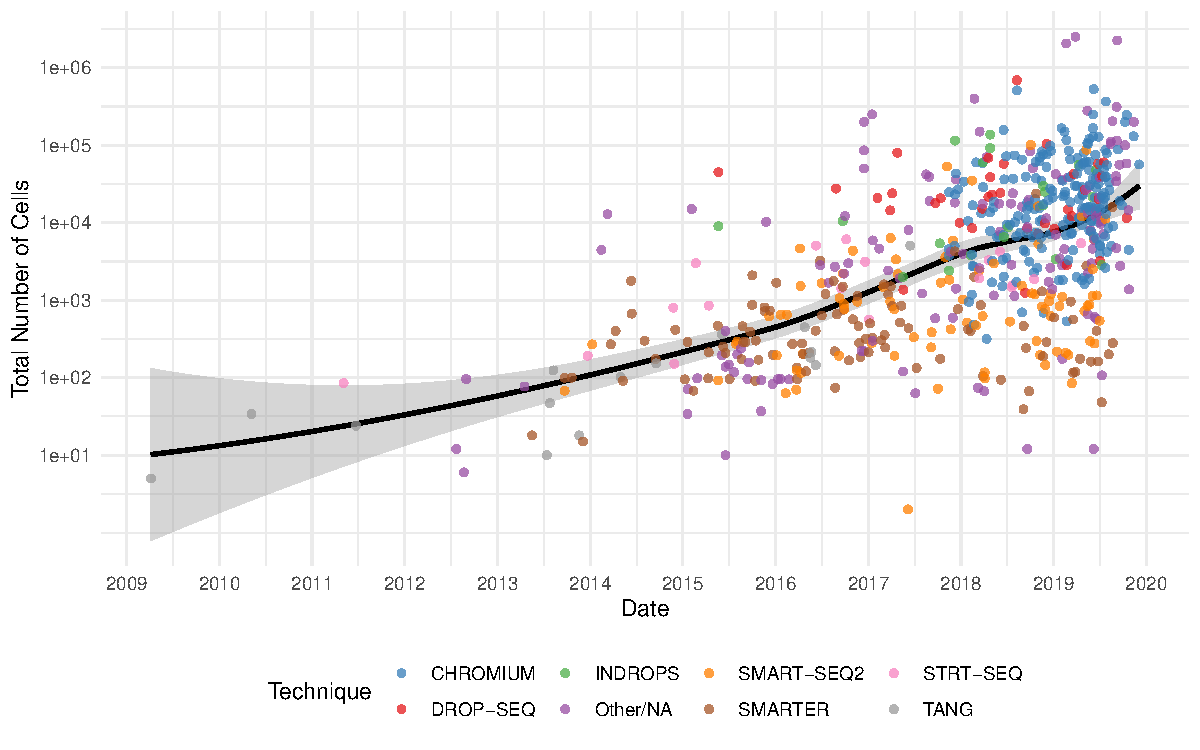
\includegraphics[width=\textwidth]{figures/intro/scStudies.pdf}
	\caption[scRNAseq Publications]{Exponential scaling of Single Cell RNAseq studies. Data from~\cite{Svensson2019curated}}
	\label{fig:scStudies}
\end{figure}

In scRNAseq, due to the low amount of starting material, many rounds of PCR amplification are required to generate sufficient material for sequencing.
However this amplification step introduces significant bias, skewing the resulting levels \parencite{Best2015Computational}.
To alleviate this unique barcodes named UMIs (unique molecular identifier) can be included in each poly-dT probe, in addition to the unique barcode for each cell (1 per bead) \parencite{Kivioja2012Counting,Islam2014Quantitative}.
This enables each original mRNA molecule to be counted as a single molecule, in effect providing an absolute count of molecules rather than relative abundance as in standard bulk RNAseq.
However, UMIs do not alleviate bias due to preferential sampling of molecules by RT or PCR primers \parencite{Kou2016Benefits}.
In addition, as the UMI and cellular barcode is on the 3' end of the transcript, after fragmentation only the fragments at the 3' end will be sequenced.
This bias is in addition to the 3' bias from polyA selection \parencite{Wan2012Modeling, Lahens2014IVTseq}.
This 3' bias precludes analysis of transcript isoforms as only the 3' end of the fragment is sequenced (as most transcripts share the 3' UTR, and the 5' read contains only the UMI and cell barcode).
However, some isoform information is available due to the use of alternative 3' UTRs (and possibly by internal polyA priming), if pseudo-alignment is used to generate transcript compatibility counts \parencite{Nam2002Oligo, Ntranos2019discriminative}.

Despite what the name suggests, some ``single cells'' will actually be multiple cells, due to two (or more) cells being captured into the same droplet or well, named ``doublets''.
The doublet rate is determined by concentration of cells in the solution / flow rate into the droplets.
By Poisson sampling a flow rate can be calculated to minimise doublets but also balance the cost of empty beads.
The doublet rate can be determined experimentally by mixing single cells from two different species, in which case double species encapsulations can be detected by the different gene sequences (and the total number of doublets calculated as double that) \parencite{Macosko2015Highly}.
 Doublets can also be detected by natural genetic variation when multiplexing multiple genetically distinct individuals of the same species \parencite{Kang2018Multiplexed}.
Artificial genetic variation can also be added by using oligonucleotide-tagged antibodies \parencite{Stoeckius2018Cell}.
Recently a method using whole-transcriptome pre-indexing was proposed, enabling overloading of droplets and a corresponding massive increase in throughput \parencite{Datlinger2019Ultrahigh}.
A number of computational tools have also been created to attempt identification of doublets by simulating artificial doublets \parencite{Wolock2019Scrublet, McGinnis2019DoubletFinder}.
Another way in which mRNA can cross contaminate across cells is if damaged cells leak mRNA into the solution which is then captured.



\subsection{Spatial Sequencing}
A disadvantage in most single cell RNAseq methods is the loss of spatial information during cell dissociation and isolation.
New methods have been developed to combine the spatial advantages of In Situ Hybridisation and the transcriptome wide nature of scRNAseq.
One type of method ``in situ sequencing'' typically uses rolling circle amplification of an mRNA target resulting in a DNA nano-ball which is sequenced by ligation, achieving a resolution of 0.5-1$\mu$m for up to 1,000 genes \parencite{Lee2014Highly, Wang2018Threedimensional, Qian2018spatial}.
Another approach ``spatial transcriptomics'' uses a spatially barcoded bead array which captures mRNA from an overlaid tissue, enabling quantification of all genes but with lower spatial resolution (2-100$\mu$m) than in situ sequencing \parencite{Stahl2016Visualization, Rodriques2019Slideseq, Vickovic2019Highdefinition}


\subsection{Nascent RNA Sequencing}
Although we say the previous methods measure ``expression'' we are actually measuring the total mRNA, which is the cumulative result of transcription minus mRNA degradation.
Methods such as GRO/PRO/NET-seq allow profiling of nascent mRNA, revealing which genes are being transcribed at a specific time-point \parencite{Core2008Nascent, Churchman2011Nascent, Mahat2016Basepairresolution}.


\subsection{Proteomics}
Given that we (mostly) ultimately care about \emph{protein} function, using mRNA as a proxy for this deserves some caveats and justification.
Quantification of the full proteome, either by mass-spectrometry approaches or by nanopore protein sequencing, hold promise (with proteins being present in higher copy number than mRNA) but has yet to be fully realised \parencite[Reviewed in][]{Specht2018Transformative,Marx2019dream}.
Whilst there are many factors resulting in a decoupling of mRNA and protein levels, protein levels are largely determined by mRNA concentrations \parencite[Reviewed in][]{Liu2016Dependency}.




%%%%%%%%%%%%%%%%%%%%%%%%%%%%%%%%%%
%%%%%%%%%%%%%%%%%%%%%%%%%%%%%%%%%%
%%%%%%%%%%%%%%%%%%%%%%%%%%%%%%%%%%


\section{Gametogenesis}
Gametogenesis is the process by which primordial germ cells develop into either spermatozoa in the male (spermatogenesis) or ovum in the female (oogenesis).
Whilst equally important to spermatogenesis, oogenesis is studied far less (1,099 vs 359 articles indexed in PubMed 2018).
This is likely partially due to difficulties in studying oogenesis compared to spermatogenesis.
In oogenesis prophase I up to diplotene occurs in the ovary of the fetus before birth at which point meiosis is arrested (``Dictyate''), making experiments more challenging.

\subsection{Testis Anatomy}
Whilst the fundamental features of spermatogenesis and oogenesis are the same, spermatogenesis is organised into a specific structure.
The testis is composed of seminiferous tubules surrounded by somatic accessory cells such as Leydig cells which produce testosterone.
Germ cells are located within the tubule supported by a somatic cell type named Sertoli cells.
The germ stem cells are located at the basal surface next to the tubule wall, and more differentiated germ cells are located progressively inwards towards the lumen/apical surface of the tubule (figure~\ref{fig:histology}).

\begin{figure}[H]
	\centering
	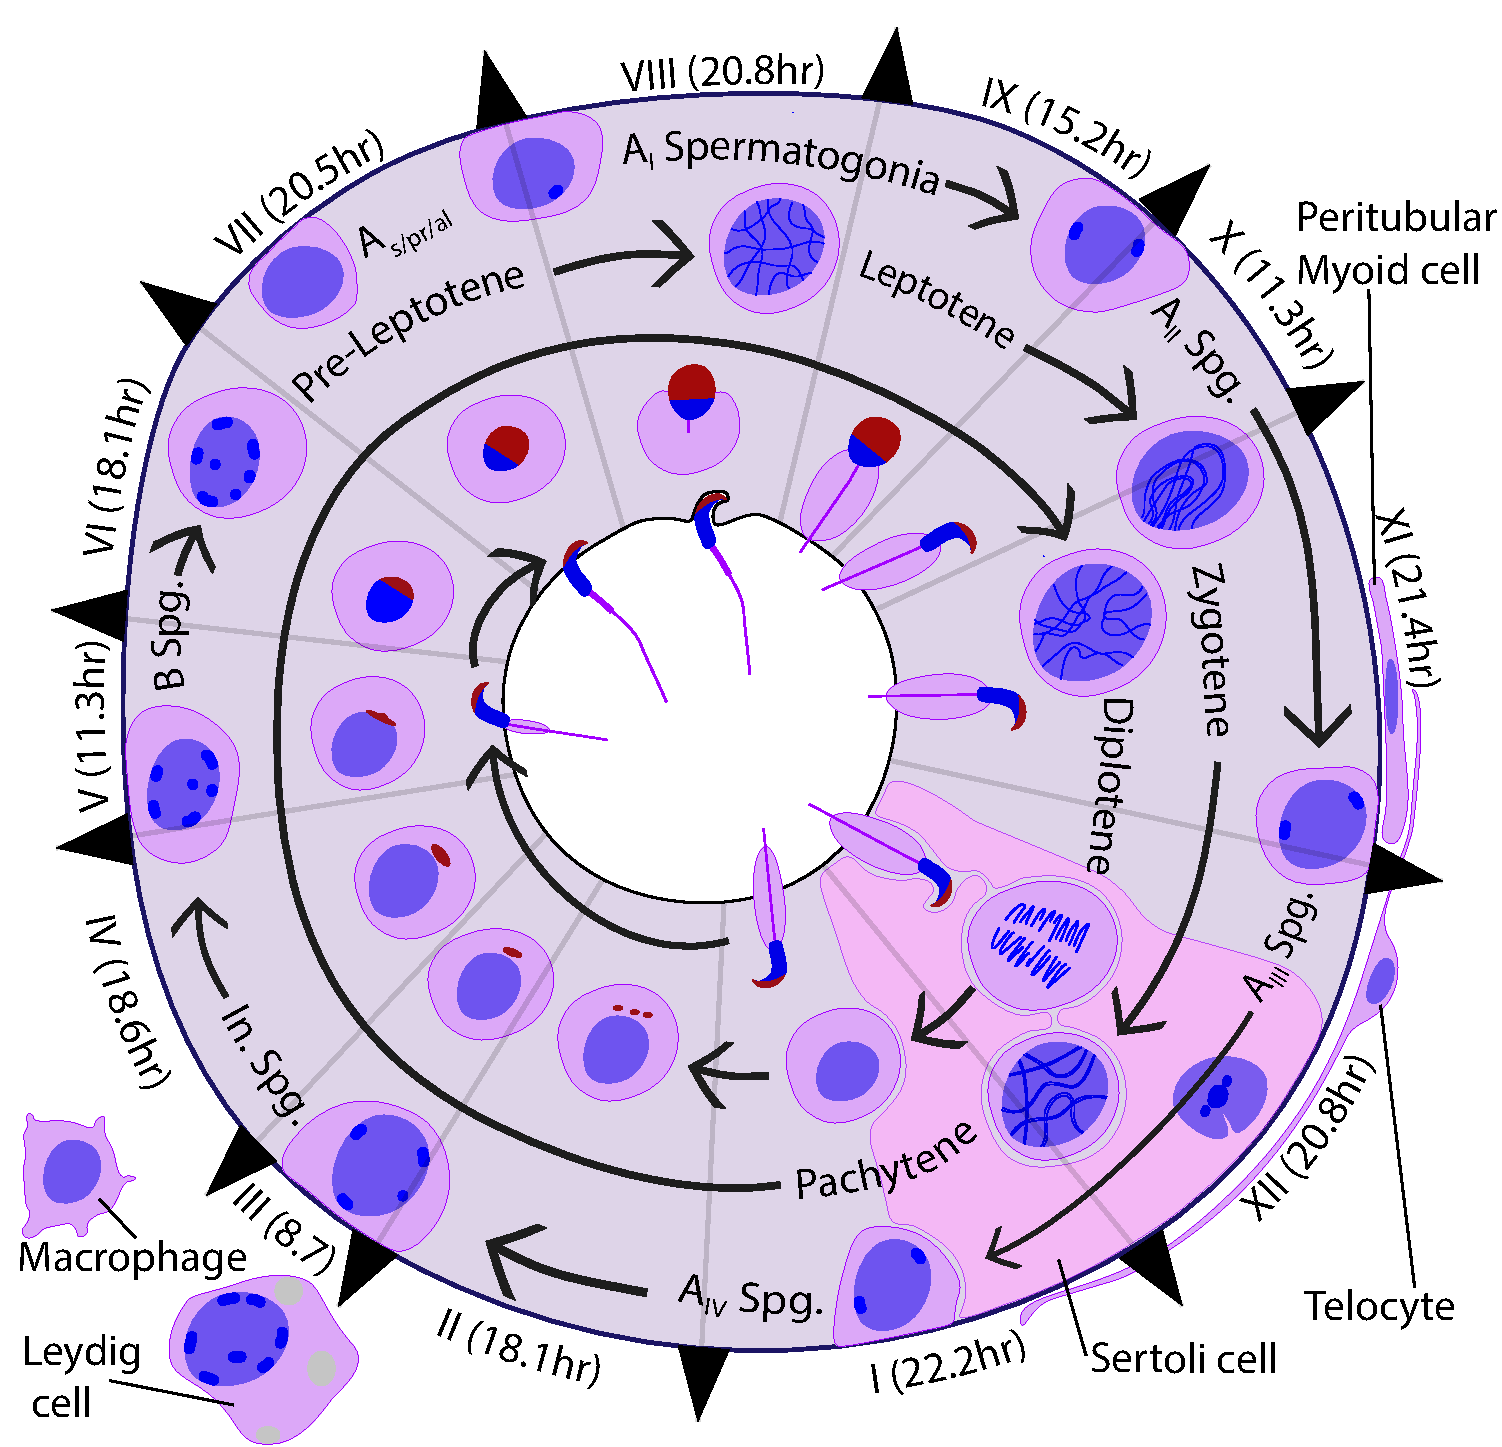
\includegraphics[width=\textwidth]{figures/intro/testis_cycle_anatomy.pdf}
	\caption[Testis Anatomy]{The cycle of the seminiferous epithelium shown within a cross section of a seminiferous tubule.
To simplify the diagram no intracellular cytoplasmic bridges are shown and only one type of each cell is shown.
As/pr/al cells actually exist in all stages.
In any given tubule cross section only the cell types from a single stage will be present in mice.
Stage numbers are shown around the perimeter of the tubule demarcated by black triangles.
In. : Intermediate, Spg. : Spermatogonia.
Stage timings from \cite{Oakberg1956Duration}, Sertoli features from \cite{Hess2015Sertoli}, Chromosome morphology during prophase I from \cite{Link2019Meiotic}, general cycle descriptions from \cite{Monesi1978Chapter, Ahmed2009Staging, Meistrich2013Assessment, Oakberg1956description, Hess2008Spermatogenesis, Nakata2015Quantitative, Muciaccia2013Novel, Osuru2014acrosomal, Lara2018Testis, Junqueira2005Basic}.}
	\label{fig:histology}
\end{figure}

Within a given region of tubule, entry into spermatogenesis is coordinated such that each developing germ cell belongs to a cohort of the same stage.
The rate of entry is precisely timed (every 8.6 days in mice) and shorter than the total developmental time (35 days in mice, >70 in humans) such that in any given tubule section different generations of germ cells occur in layers of particular cell type combinations (figure \ref{fig:histology}, \cite{Oakberg1956Duration,Clermont1969Duration, Heller1969Human}).
This is called the cycle of the seminiferous epithelium and it is possible to stage each combination of cells using periodic acid‐fuchsin sulfurous acid staining (14 combinations in rat, and 12 in mouse) \parencite{Leblond1952Spermiogenesis, Leblond1952Definition, Oakberg1956description}.
The cycle starts at a different time laterally along the tubule (in a so called ``wave''), ensuring continuous production of sperm, although the very first wave is synchronous - a property sometimes used to purify or enrich for specific stages.

\subsection{Spermatocytogenesis}
Prior to meiosis there are a number of \emph{mitotic} divisions, amplifying the true spermatogonial stem cell \parencite{Oakberg1971Spermatogonial, Huckins1971spermatogonial}.
The first set of these divisions occur asynchronously between stage stages X and II \parencite{Rooij2001Proliferation}.
There are up to four or five divisions in this first proliferation and the resulting cells are named $A_{single}$, $A_{paired}$, $A_{aligned-4}$ $A_{aligned-8}$, $A_{aligned-16}$.
At stage VIII all the $A_{aligned}$ cells differentiate (without division) into $A_1$ cells which are considered committed to the meiotic program and now divide in synchrony with the stages of the seminiferous cycle \parencite{Rooij2000All}.
This commitment step is induced by a pulse of retinoic acid (Vitamin A metabolite), which induces expression of the Stra8 transcription factor in these cells (and pre-leptotene cells which occur in the same stage) \parencite{Griswold2012Initiating, Lin2008Germ, Zhou2008Expression, Hogarth2015Processive, Griswold2015Spermatogenesis}.
A Vitamin A deficient diet results in lack of progression to $A_1$ spermatogonia, enabling an additional method to generate synchronised cells \parencite{Thompson1964Vitamin}.
$A_1$ cells divide by mitosis into $A_2$, then $A_3$, and $A_4$ all of which are indistinguishable morphologically but occur at different stages of the seminiferous cycle \parencite{Rooij2000All}.
$A_4$ cell divide into ``In'' cells (with intermediate levels of heterochromatin) and then into spermatogonial B cells before a final mitosis generates pre-leptotene spermatocytes \parencite{Rooij2000All}.

Meiosis is preceded by DNA replication much like in mitosis, and so initiates from cells that are 2n, 4c (n = ploidy / number of centromeres; c = number of chromosomes).

\subsection{Prophase I of Meiosis I}
During meiosis there is an extended prophase I (lasting 14 days in mice), which is itself divided into a number of stages: Leptotene (thin ribbon), Zygotene (union ribbon), Pachytene (thick ribbon), and Diplotene (double ribbon) - originally defined by the morphology of the chromosomes through a light microscope (sometimes suffixed -nema using the greek for ``thread'' instead of ``ribbon'') \parencite{DeWiniwarter1900Recherches, Gregoire1907formation, Wilson1912Studies, Zickler1998leptotenezygotene}.

However, with the discovery of the synaptonemal complex (figure \ref{fig:synaptonemal_complex}, a proteinaceous scaffold that forms along the chromosomes, \cite{Moses1956Chromosomal, Fawcett1956FINE}), the stages are also now defined by the configuration of this structure \parencite{Zickler2015Recombination}.
Lepotene being the stage in which the lateral elements form along the axis of homologous chromosomes, Zygotene starts at the formation of the first transverse filaments and the central element between the homologous chromosomes \parencite{Moens1968structure}, Pachytene is defined as the stage in which all chromosomes (excepting the sex) are fully synapsed, and Diplotene when the synaptonemal complex starts to disassemble \parencite{Moses1958Relation, Moses1977Synaptonemal}.
The lateral elements are formed of SYCP2 (Red1 in \textit{S. cerevisiae}) \& SYCP3 proteins, whereas the central element is formed of SYCE1, SYCE2, SYCE3, SIX6OS1, and TEX12, with SYCP1 forming the transverse elements connecting the two \parencite[reviewed in][]{Zickler2015Recombination, Gao2018Zipping, Kaniecki2018change, Dunce2018Structural}.
The formation of the axis is dependent on a meiosis specific cohesin complex (composed of REC8, RAD21L, SMC1B, STAG3) which encircles the sister chromatids during premeiotic S phase \parencite[reviewed in][]{Rankin2015Complex, Ishiguro2019cohesin}.

\begin{figure}[H]
	\centering
	\includegraphics[width=\textwidth]{figures/intro/synaptonemal_complex.pdf}
	\caption[Synaptonemal Complex]{Schematic of the synaptonemal complex at different stages during Prophase I~\parencite[based on ][]{Gaysinskaya2018MOESM1, Gaysinskaya2018Transient, Cohen2010Predicting, Bolcun-Filas2012Chapter, Hughes2018Female, Cahoon2017Superresolution}}
	\label{fig:synaptonemal_complex}
\end{figure}

At the start of prophase I in Leptotene, SPO11, a conserved topoisomerase like protein, acts with mTopVIB (GM960 in mice) to create programmed double-strand breaks (DSBs) \parencite{Sun1989Doublestrand, Keeney1997MeiosisSpecific, Bergerat1997atypical, Cole2012Homeostatic, Vrielynck2016DNA, Robert2016TopoVIBLike, Li2019highresolution}.
Like other topoisomerases the two SPO11 molecules form covalent bonds with each end of the DNA \parencite{Neale2005Endonucleolytic}.

The activity of SPO11 depends on pre-DSB recombinosomes containing MEI4, REC114, IHO1 (aka CCDC36, MER2) and ANKRD31 which are bound to unsynapsed axes via HORMAD1/2 \parencite{Kumar2010Functional,Panizza2011Spo11Accessory, Stanzione2016Meiotic, Kumar2018Mouse, Papanikos2019Mouse, Boekhout2019REC114}.
However most DSBs are inflicted on the DNA within one of the many loops that form a linear array, rather than the DNA secured to the central axis from which the loops emanate.
Therefore, before DSBs occur, the sites destined to be broken are brought to the axis to form a tethered loop axis complex (figure \ref{fig:synaptonemal_complex}) \parencite{Blat2002Physical,Panizza2011Spo11Accessory}.
In \textit{S. cerevisiae} Spp1 provides the link by binding both H3K4me3 and Mer2 (IHO1), however the mouse orthologue CXXC1 does not appear to play the same role, and so it is unclear which protein(s) provide this link in mice \parencite{Acquaviva2013COMPASS,Sommermeyer2013Spp1,Tian2018CXXC1}.
MEI1 is also required for DSBs, and WDR61 is hypothesised to be required as it is a homologue of Ski8/Rec14 which is required in \textit{S. cerevisiae} \parencite[reviewed in][]{Kumar2010Initiation, Lam2015Mechanism}.
pre-DSB recombinosome recruitment also depends on meiotic cohesin \parencite{Bhattacharyya2019Prdm9}.

The DSB lesions are initially processed in much the same way as DSBs in mitotic cells: they are rapidly recognised by CtIP-(SAE2)-activated MRN complex (MRE11, RAD50, NBS1), which possesses 3'-5' nuclease activity.
They are then further resected by either the 5'-3' exonuclease EXO1, or DNA2 nuclease with the BTRR complex (BLM (SGS1) helicase, TOP3A, RMI1, RMI2 \parencite{Daley2014Multifaceted}) resulting in the release of SPO11 bound oligos \parencite[Reviewed in][]{Symington2014End, Schiller2014Structural, Lam2015Mechanism}).
MRN recruits the ATM kinase which in turn activates a cascade of DNA damage response activities including phosphorylation of the histone variant H2AX \parencite{Marechal2013DNA}.
RPA then coats the single stranded DNA, but is replaced by RAD51 and the meiosis specific protein DMC1, with the aid of BRCA2 \parencite{Liu2010Human, Jensen2010Purified, Shi2019Dual}.
MEIOB and SPATA22 are RPA homologues that are also recruited to DSBs, but their function is unknown \parencite{Xu2017Meiosisspecific}.


\begin{figure}[H]
	\centering
	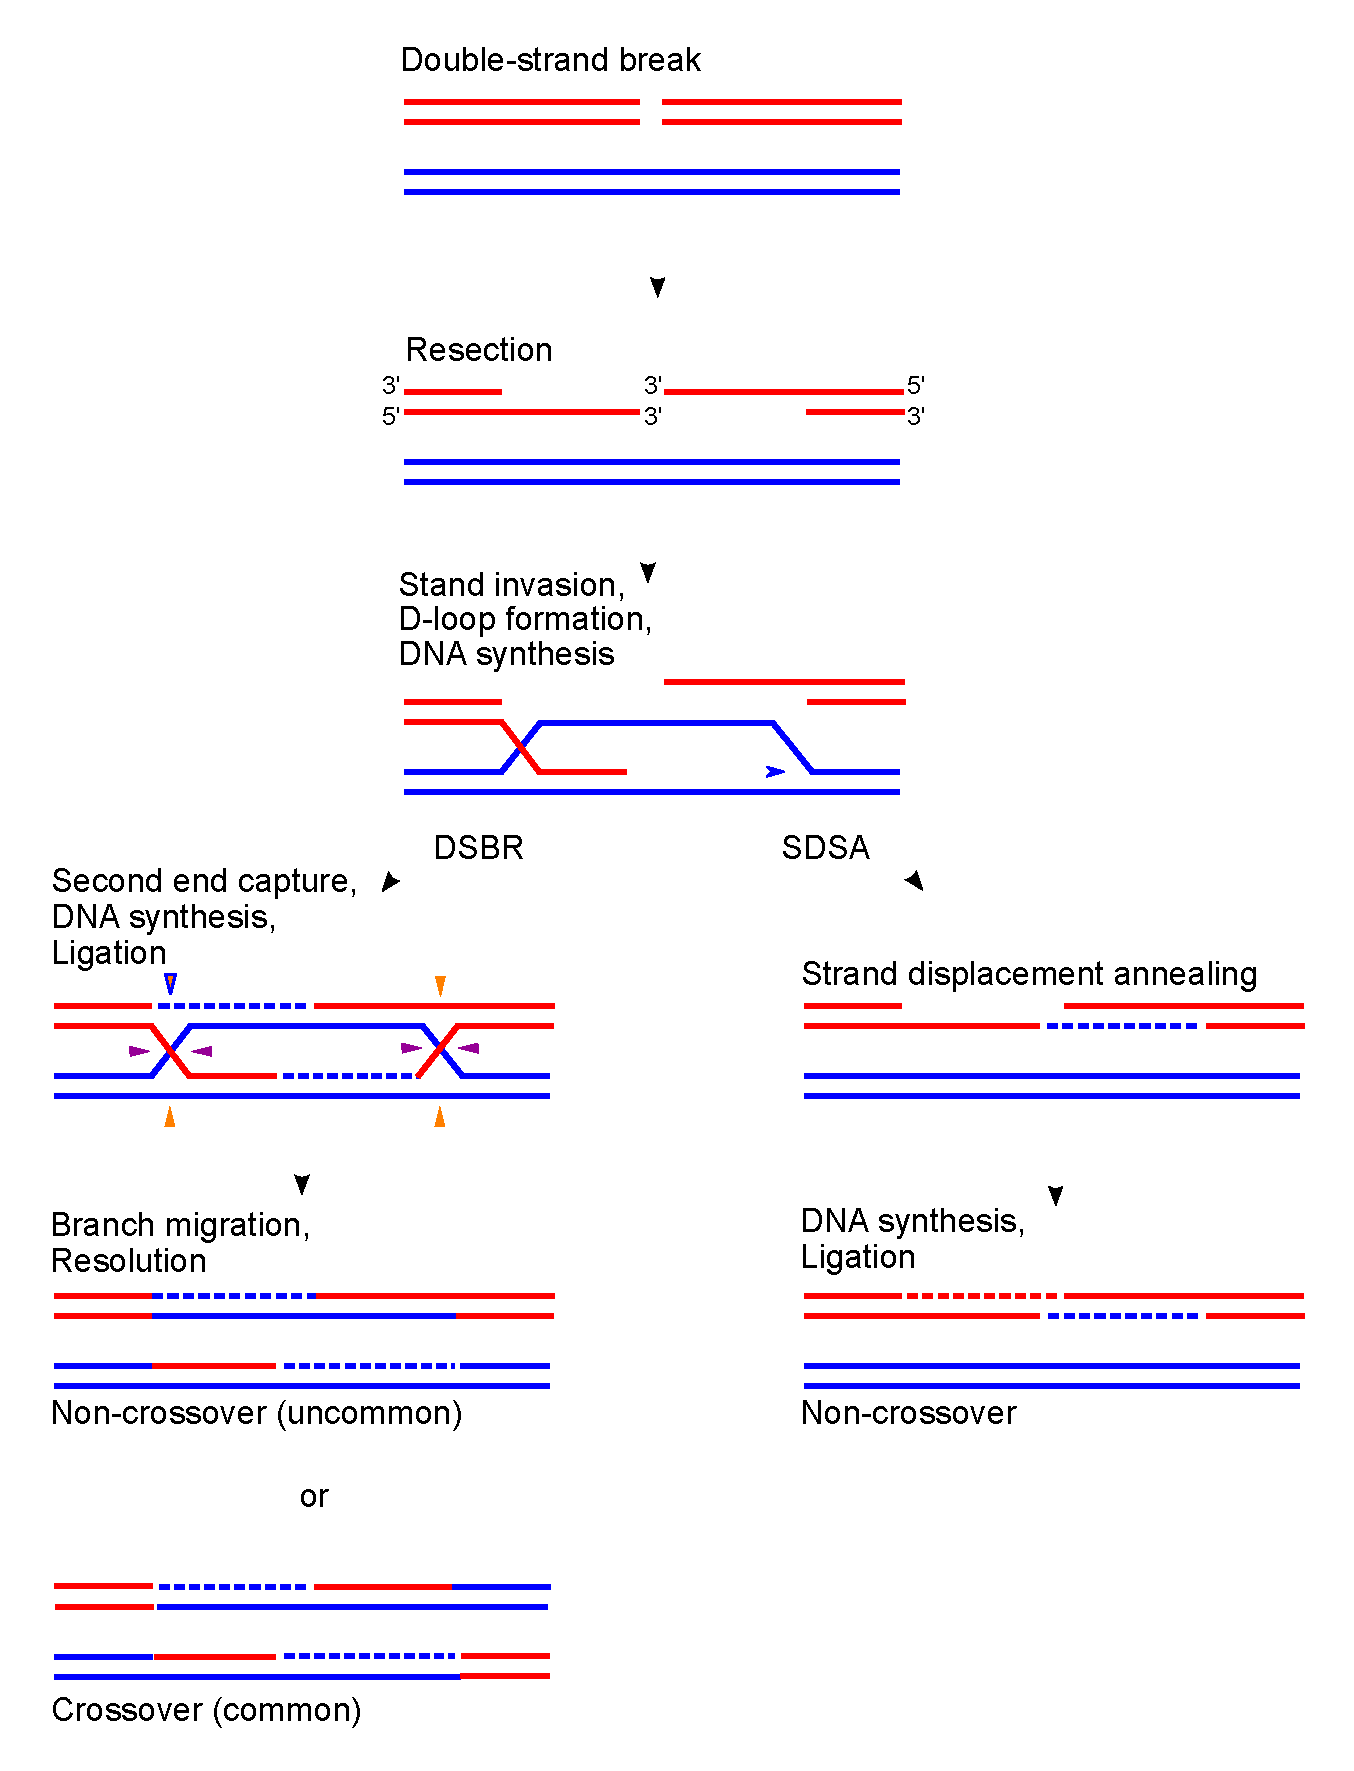
\includegraphics[width=0.6\textwidth]{figures/intro/recombination.pdf}
	\caption[Molecular Recombination]{Schematic of the recombination process. By Wikipedia user User:Emw2012 (CC BY-SA 3.0), based on \cite{Sung2006Mechanism}}
	\label{fig:molecular_recombination}
\end{figure}

RAD51 and DMC1, along with other helper proteins, form a right handed bipolar helical filament (where DMC1 is oriented at the broken end, with 3bp per monomer), able to invade the homologous chromosome to search for a homologous template for repair \parencite{Sehorn2004Human, Cloud2012Rad51, Brown2015Small, Brown2015DNA, Crickard2018Spontaneous}.
This filament is brought / binds to duplex DNA (perhaps helped by RAD51AP1, PALB2, or HOP2-MND1, \cite{Petukhova2005Hop2}) and probes for homology using base-flipping - where the nucleoside is rotated out of the double helix \parencite{Gupta1999Rapid, Folta-Stogniew2004Exchange}.
This search likely involves a combination of 3D search, 1D sliding, and length dependent (>8bp) recognition of micro-homology, reminiscent of Cas9 search \parencite{Ragunathan2012RecA,Forget2012Singlemolecule,Renkawitz2013Monitoring,Qi2015DNA,Lee2015Base}, \parencite[reviewed in][]{Barzel2008Finding, Renkawitz2014Mechanisms, Greene2016DNA, Kaniecki2018change, Haber2018DNA}.
The filament is likely released from non-homologous interactions by ATP hydrolysis \parencite{Lee2016ATP}, and is stabilised by MCMDC2 for homologous interactions \parencite{McNairn2017Repair}. 

At this point the homologous chromosomes are aligned at a distance of approximately 400nm with the invading filament visible as an interaxis bridge.
As the synaptonemal complex forms, nucleated at sites designated to become crossovers, the axes are brought closer together to a distance of around 100nm \parencite[reviewed in][]{Zickler2015Recombination}.

Successful single strand invasion causes a displacement (D) loop (coated by RPA), and a Holliday junction (figure \ref{fig:molecular_recombination}).
DNA synthesis proceeds using the homologous template DNA, possibly by polymerase eta \parencite{McIlwraith2005Human, Kawamoto2005Dual} and then branch migration (catalysed by RAD54, RECQ1, and BLM) causes either D loop extension or dissociation \parencite{Bugreev2006Rad54,Bugreev2008RECQ1, Mazina2012Polarity}.
In the case of dissociation, the newly synthesised strand can re-anneal to the resected DNA overhang to be repaired by further DNA synthesis and ligation, forming a non-crossover gene conversion (a processed called Synthesis Dependent Strand Annealing, figure \ref{fig:molecular_recombination}).
In the case of loop extension, second end capture (catalysed by RAD52, \cite{Sugiyama1998DNA, Sugiyama2006Rad52mediated, McIlwraith2008DNA, Lao2008Rad52}) followed by DNA synthesis and ligation results in a double Holliday Junction (dHJ).
This can also result in a non-crossover gene conversion in a process called double-junction dissolution, in which convergent branch migration is followed by de-catenation (catalysed by BLM-TOPO3A, \cite{Wu2003Bloom, Bizard2014Dissolution}).

MUS81-EME1/EME2 can cleave dHJs, as can SLX1-SLX4 and GEN1 when there is no nuclear envelope \parencite[reviewed in][]{Wyatt2014Holliday}.
These DNA nickases can generate both crossovers and non-crossovers depending on whether they nick symmetrically or asymmetrically respectively (figure \ref{fig:molecular_recombination}).
In meiosis the MLH1-MLH3 heterodimer (MutLγ) is recruited to sites with MutSγ, and can resolve the dHJ into crossover products by asymmetric nuclease activity \parencite{Zakharyevich2012Delineation} and \parencite[reviewed in][]{Hunter2015Meiotic, Gray2016Control, Manhart2016Roles, Toledo2019mutation}. 

MutSγ is a member of a group of proteins, named ZMM proteins, which help to stabilise double Holliday junction intermediates to promote the crossover pathway.
This includes MSH4 and MSH5 that as a heterodimer (MutSγ) form a sliding clamp around HJs, HFM1 (MER3), SYCP1 (ZIP1), SHOC1 (ZIP2), SPO16, TEX11 (ZIP4), HEI10 and RNF212 (ZIP3) \parencite[reviewed in][]{Pyatnitskaya2019Crossing}.

% HORMAD1/2, MORC2B

The locations at which these double-strand breaks occur are not uniformly distributed across the genome, although the nonuniformity and locations vary by species.
\textit{Caenorhabditis elegans} has quite a uniform distribution with little fine scale structure (Gini coefficient of 0.28) \parencite{Rockman2009Recombinational, Kaur2014Crossover}.
\textit{Drosophila melanogaster} is similar with a Gini coefficient of 0.5 \parencite{Chan2012GenomeWide, SmukowskiHeil2015Recombining}.
In other species recombination occurs at a small subset of the genome in clusters called ``recombination hotspots'', originally named from work on the Chi sequence which can specify recombination in E. coli \parencite{Lam1974RecMediated, Myers1994RecBC}.
\textit{Saccharomyces cerevisiae} has a Gini coefficient of 0.64, with recombination occurring in hotspots that are 50-300bp, typically (88\%) overlapping promoters (in contrast to Drosophila), and are nucleosome depleted \parencite{Baudat1997Clustering, Wu1994Meiosisinduced, Mancera2008Highresolution, Pan2011Hierarchical, Lam2015Nonparadoxical}.

Recombination in humans occurs in hotspots 1-2kb in width that, unlike yeast, are not usually at promoters \parencite{Jeffreys2001Intensely}.
Genome wide locations of these hotspots has been inferred from increasingly high resolution genetic maps derived from linkage disequilibrium patterns \parencite{McVean2004finescale, Myers2005FineScale, TheInternationalHapMapConsortium2007second, Coop2008HighResolution} and pedigrees which enable sex-specific inference \parencite{Kong2002highresolution, Kong2010Finescale, Kong2014Common, Bherer2017Refined, Halldorsson2019Characterizing},

These maps of hotspots lead to the discovery of a 7-mer (CCTCCCT) associated with recombination rate \parencite{Myers2005FineScale}, which appeared to be causal \parencite{Jeffreys2002Reciprocal}.
This motif was later extended to the 13-mer CCNCCNTNNCCNC \parencite{Myers2008common} which was found to match the predicted binding motif of PRDM9 \parencite{Myers2010Drive, Baudat2010PRDM9, Parvanov2010Prdm9, Berg2010PRDM9}.
In addition to the zinc finger array (which specifies the binding motif of the protein), \textit{Prdm9} also has a KRAB domain, an SSXRD domain, and a PR/SET methyltransferase domain.
The methyl-transferase domain is able to catalyse both H3K4me3 and H3K36me3, and both of these marks are required for its role in positioning DSBs \parencite{Powers2016Meiotic, Diagouraga2018PRDM9}.

\textit{Prdm9} is the founding member of a family of KRAB zinc finger genes \parencite{Birtle2006Meisetz}.
There are around 600 such genes in mice (only \textasciitilde8 in birds), most of them likely to be involved in repressing retrotransposons by recruiting KAP1 (aka TRIM28) but PRDM9 does not have this ability \parencite{Imbeault2017KRAB, Bruno2019Arms}.
\textit{Prdm9} is among the fastest evolving regions of the genome \parencite{Oliver2009Accelerated}, and consistent with this the locations of hotspots in Chimp are not shared with Humans \parencite{Wall2003Comparative, Ptak2004Absence, Ptak2005Finescale, Winckler2005Comparison}.
However, general features of the recombination landscape are the same in Chimps, including increasing heat at the sub-telomeres, hotspot width and intensity, and rate depression within gene bodies \parencite{Auton2012FineScale}.
Similar results have also been obtained in mice \parencite{Paigen2008Recombinational, Brunschwig2012FineScale, Booker2017Recombination}, with some studies utilising the increased feasibility of experimental manipulation of mice to use alternative detection methods such as assaying the intermediates of recombination such as ssDNA bound DMC1 \parencite{Smagulova2011Genomewide, Khil2012Sensitive, Smagulova2016evolutionary}, SPO11 oligos \parencite{Lange2016Landscape}, as well as using single sperm sequencing of hybrids with genetic differences (much greater than in humans)\parencite{Hinch2019Factors}, and linked reads \parencite{Dreau2019Genomewide}.
DMC1 mapping has also been applied to human samples revealing the contribution of individual \textit{Prdm9} alleles \parencite{Pratto2014Recombination} and recently low coverage high throughput single sperm sequencing has also been used on human samples \parencite{Bell2019Insights}.

In Canids recombination rate is even more unequally distributed than in humans, is similarly increased towards the subtelomeres (especially in males), but is directed towards CpG rich sequences such as promoters as in yeast \parencite{Auton2013Genetic, Campbell2016PedigreeBased}; consistent with the loss of functional \textit{Prdm9} in the Canidae family \parencite{Munoz-Fuentes2011Prdm9}.
Similarly in birds, which also lack a functional \textit{Prdm9}, recombination hotspots exist but are conserved across species diverged by tens of millions of years and are enriched at CpG islands including transcription start sites - perhaps driven by nucleosome depletion and so increased accessibility to the recombination machinery \parencite{Singhal2015Stable}.
Plants also lack \textit{Prdm9}, and again crossovers are enriched at promoters, and other promoter associated marks such as H2A.Z and H3K4me3 \parencite{Choi2013Arabidopsis, Marand2017Meiotic}.

Furthermore, knockout of \textit{Prdm9} in mice causes hotspots to relocate to promoters \parencite{Brick2012Genetic}.
\textit{Prdm9} B6 knockout mice are infertile, but this is not true for other strains, and one \textit{Prdm9} homozygous null female human has had three healthy children \parencite{Hayashi2005histone, Mihola2019Histone, Narasimhan2016Health}.
A partial relocation to promoters is seen in \textit{Ankrd31} knockouts \parencite{Boekhout2019REC114, Papanikos2018ANKRD31}.
\textit{Prdm9} is also the cause of infertility in the F1 male hybrids of crosses between \textit{Mus musculus domesticus} (B57BL/6J) and \textit{Mus musculus musculus} (PWD/Ph, differing by only a single finger), representing the only known mammalian speciation gene \parencite{Forejt1974Genetic, Mihola2009Mouse}.
The cause of this sterility was recently revealed by engineering mice with a humanized version of \textit{Prdm9}, which rescues the fertility of F1 hybrids \parencite{Davies2016Reengineering}.
Hotspots are gradually eroded by biased gene conversion (the colder allele is used as a template to repair the double strand break occurring on the hotter template), resulting in the paradox of hotspot existence \parencite{Boulton1997hotspot, Coop2007Live, Myers2010Drive, Baker2015PRDM9}.
Using a humanised zinc finger increases the symmetry of DSB formation, and this increased symmetry is associated with increased synapsis and fertility.
Additionally asymmetric hotspots have greater DMC1-ChIPseq signal compared to H4K3me3 (a measure of PRDM9 activity) suggesting delayed repair at PRDM9-asymmetric sites.
This work also implies that PRDM9 plays a role not just in DSB positioning but DSB repair in a manner depending on symmetric binding.
Further work using hybrid mice pedigrees and single sperm sequencing demonstrated that at sites with asymmetric PRDM9 binding, homologue templated repair was depleted compared to PRDM9-symmetric sites, showing that PRDM9 influences repair as well as positioning of DSBs \parencite{Li2019highresolution, Hinch2019Factors}.

While there are many potential binding sites for PRDM9 (>170,000 in a HEK293T overexpression system \parencite{Altemose2017map}) and hence potential crossover locations, there are only tens of thousands of hotspots \parencite{Myers2005FineScale, Pratto2014Recombination}, and only 1-2 crossovers form per chromosome in a single meiosis.
At each stage of recombination the number of potential crossover sites is reduced, and at each stage various factors influence the likelihood of a site surviving to the next stage of selection.
While PRDM9 likely deposits H3K4me3 at almost all locations it binds, at some regions such as promoters recombination is suppressed, plausibly due to poor H3K36me3 deposition or active removal of this mark \parencite{Altemose2017map}.
Sequence motifs outside the PRDM9 binding footprint also influence recombination, some acting to repress recombination by recruitment of KRAB-ZNF proteins which recruit TRIM28 which in turn deposits H3K9me3 \parencite{Altemose2017map}.
H3K9me3 is a marker of heterochromatin, which is more often found in the gene poor 'B' compartments of chromosomes and laminin associated domains, and is associated with lower PRDM9 binding and recombination \parencite{Walker2015Affinityseq,Patel2019Dynamic,Yamada2017Genomic}.
Furthermore few if any DSBs occur in the pericentromeric heterochromatin \parencite{Verver2013Role}, and disruption of H3K9me2 and non-CG DNA methylation pathways in \textit{Arabidopsis thaliana} results in increased recombination at the previously heterochromatic centromeres \parencite{Underwood2018Epigenetic}.
In mice SPO11 creates \textasciitilde250/300 DSBs in males/females \parencite{Baudat2007Regulating}.
However these numbers and direction of sex bias vary by species, for example in Lily over 2,000 DSBs are formed (as assessed by RAD51 foci counts) \parencite{Terasawa1995Localization}, while in species able to pair homologues without recombination (\textit{Drosophila melanogaster} and \textit{Caenorhabditis elegans}) only ~20-30 breaks are formed.
Resolution of a DSB as a crossover is more likely if it occurs closer to the telomere, has higher local GC content, has higher H3K4me3, and has more symmetric binding of PRDM9 \parencite{Hinch2019Factors}.
Additionally, crossovers are prevented from occurring too close to one another (interference), and at least one crossover is required per chromosome (assurance/obligate) \parencite{Fledel-Alon2009BroadScale, Hunter2015Meiotic, Otto2019Crossover}.



\subsection{Post-Pachytene Processes}
Once repair has completed without the pachytene checkpoint being activated, the synaptonemal complex dissociates and cells undergo two divisions without an intervening S phase, the first reductional (separating homologous chromosomes), the second equatorial (separating sister chromatids) \parencite{Roeder2000pachytene, Subramanian2014Meiotic, Watanabe2012Geometry}.
% cohesin, condensin, monoorient etc.

Spermatocytes then begin the biochemical and morphological changes to develop into a spermatid.
One major change is the formation of the acrosome \parencite[reviewed in][]{Buffone2016Sperm, Khawar2019Mechanism}.
In the first phase (Golgi phase, steps one to three), the Golgi creates proacrosomal vesicles that fuse to become the acrosomal vesicle (although some are created as early as late pachytene).
At step three the anexome (a cytoskeletal structure responsible for flagella beating) begins to form from the distal centriole (figure \ref{fig:Spermatids}).
There is both a proximal and distal centriole below the nucleus, each of which is a microtubule based structure of 9 radial triplet microtubules arranged in a barrel \parencite{Fawcett1969fine, Avidor-Reiss2019It}.
The anexome consists of a central pair of microtubules encircled by nine doublet microtubules connected by Nexin (``9+2'' configuration, figure \ref{fig:Spermatids}) \parencite{Linck2016axoneme, Lehti2017Formation}.
Dynein motors slide these microtubules against each other creating the beating motion required for sperm motility \parencite{Mitchison2010How}.


\begin{figure}[H]
	\centering
	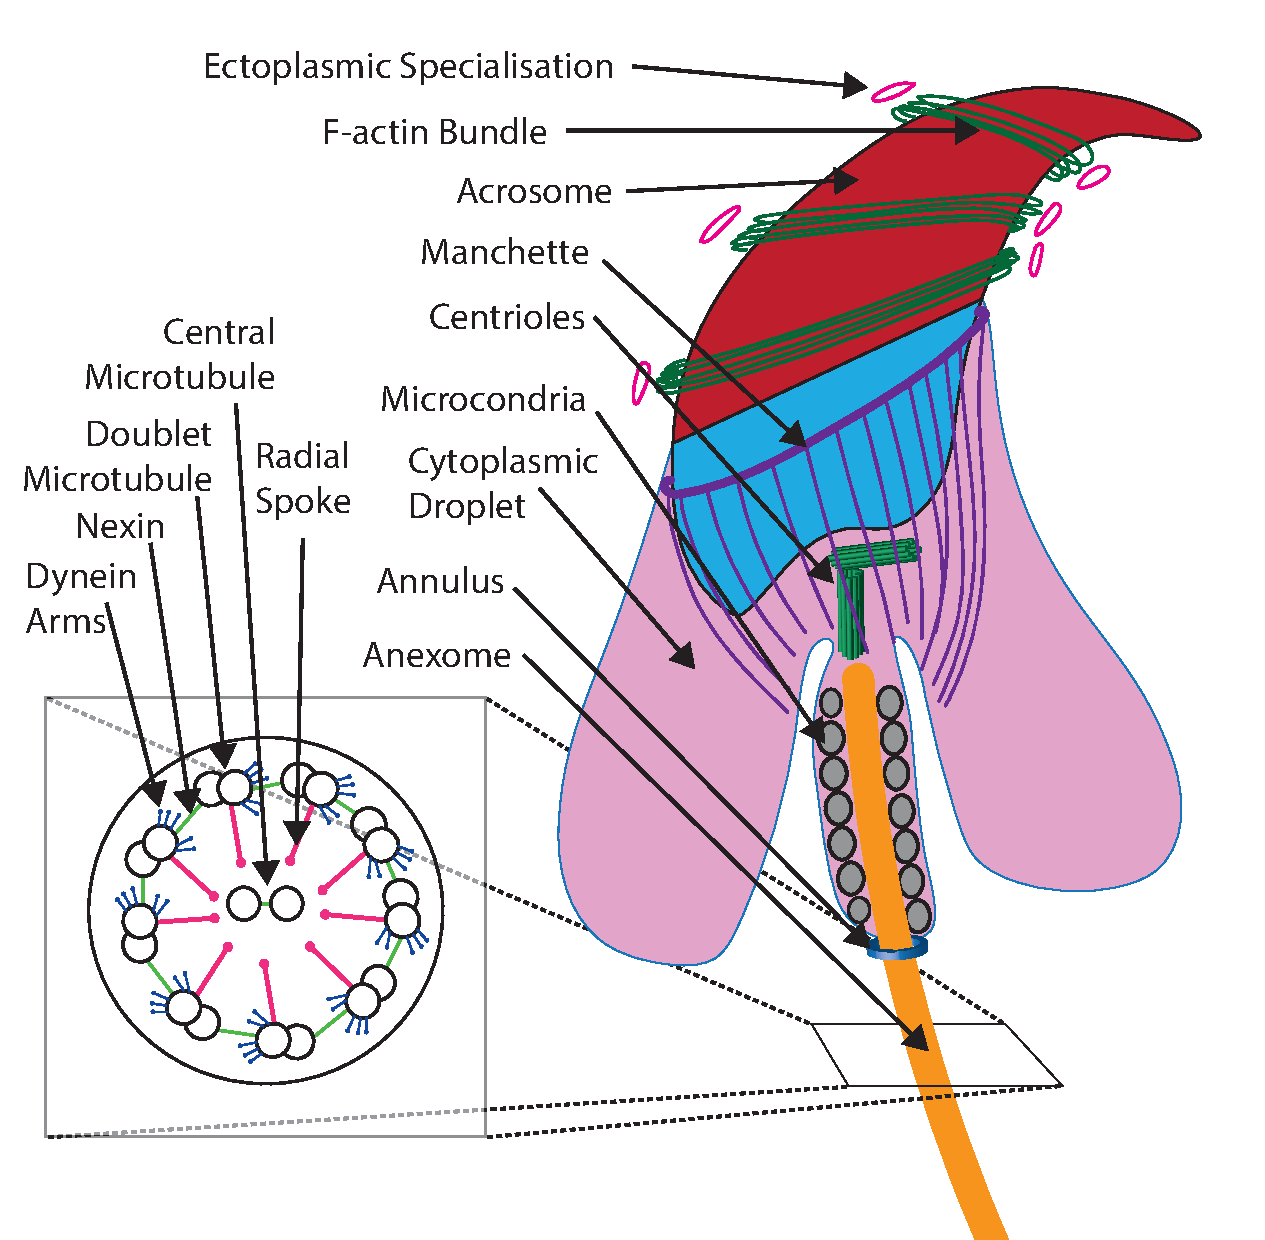
\includegraphics[width=\textwidth]{figures/intro/spermatozoa.pdf}
	\caption[Spermatids]{Schematic of subcellular structures in spermatids. Based on \parencite{Dunleavy2019cytoskeleton, Wei2018acroframosomeacroplaxomemanchette, ODonnell2012Essential, Kopera2010Sertoli, Wang2019Insight, Gunes2020Microtubular}}
	\label{fig:Spermatids}
\end{figure}


In the cap phase (steps four to seven) the acrosomal vesicle flattens to cover one side of the nucleus where it becomes anchored to the nuclear envelope by an F-actin and SAK57 (keratin5 orthologue) containing cytoskeletal structure called the acroplaxome \parencite{Kierszenbaum2003Acroplaxome, Kierszenbaum2004acrosomeacroplaxomemanchette}.

In the acrosome phase (steps eight to twelve) the acrosome orients towards the base of the tubule in close apposition to the plasma membrane.
In addition the apical ectoplasmic junction forms, anchoring the sperm head to the Sertoli cell \parencite{Wong2008Biology}.
The transient skirt like structure of the manchette also forms, consisting of a perinuclear ring important for sperm head shaping, and microtubules emanating towards the tail which are important for protein transport (figure \ref{fig:Spermatids}, \cite{Lehti2016Formation}).
Mitochondria are arranged in a helical sheath in the midpiece of the sperm, terminated at the base by the annulus which is composed of Septin octamer fibres associated with TAT1 and through which the axoneme passes \parencite{Ho2007Three, Toure2011Septins, Kuo2015SEPT12}.
Nuclear condensation begins with up to 99\% (90\%) of mice (human) histones being replaced with transition proteins and then protamines.
These short (50 a.a.) highly basic (\textasciitilde50\% arginine) proteins form a more compact toroid structure enabling a 90\% reduction in nuclear volume \parencite{Balhorn2007protamine, Ward2010Function, Yamaguchi2018Reevaluating}.
This nuclear condensation results in transcriptional cessation and therefore requires many mRNAs to be stored for long periods of time.
For example \textit{Prm1} (Protamine 1) and \textit{Smcp} (Sperm Mitochondria-associated Cysteine-rich Protein) mRNA are stored for three and seven days respectively as free ribonucleic particles before they are translated into protein on polysomes~\parencite{Cullinane2015Mechanisms, Kleene1984Translational, Kleene2004Patterns}.

In the maturation phase nuclear condensation continues while excess cytoplasm is shed as residual bodies which are digested by Sertoli cells (figure \ref{fig:Spermatids}, \cite{Lacy1962CERTAIN, Breucker1985Morphogenesis, Hermo2010Surfing}).
Spermatids are then released where they mature fully within the epididymis.
Before fertilisation the acrosome reaction occurs in which the outer acrosomal membrane fuses with the sperm plasma membrane, releasing the hydrolytic acrosomal enzymes to aid in fertilisation \parencite{Jin2011Most}.






\section{Prior Work}

A number of previous studies have measured spermatogenic gene expression.
Some studies such as GTEx (Genotype-Tissue Expression), HPA (Human Proteome Atlas), and FANTOM (Functional Annotation Of Mammalian genome) consortia have transcriptionally profiled many whole tissues in humans using RNAseq~\parencite{Mele2015Human,Uhlen2015Tissuebased,Uhlen2016Transcriptomics}.
This data enables the identification of tissue specific genes and hence a preliminary list of proteins which could be involved in meiosis.
 However, the testis is a complex amalgamation of different cell types and bulk tissue sequencing can generally not resolve the gene expression for different cell types instead resulting in a proportion weighted average.
The relative inability to faithfully culture mammalian meiotic cells in vitro has also hampered the ability to generate higher resolution time-course data \parencite{Zhou2016Complete, Hikabe2016Reconstitution}.

Nonetheless a number of techniques have been developed to improve on whole tissue resolution.
For example the initial wave of spermatogenesis is somewhat synchronous and so sampling during this time could in theory yield homogeneous cell types/stages.
However it is likely there is some variation in synchronicity resulting in impure samples and uncertain classification~\parencite{Laiho2013Transcriptome,Ball2016Regulatory}.
Some studies have combined this approach with an in silico deconvolution or machine learning algorithms~\parencite{Margolin2014Integrated,Li2013Identification}.
One study utilised the greater synchrony of meiosis in fetal ovaries in combination with germ cell depleted mutant mice to partially delineate the meiotic prophase gene regulatory programme~\parencite{Soh2015Gene}.
Other approaches include either size based centrifugal sorting~\parencite{Soumillon2013Cellular,Buard2009Distinct,Grabske1975Centrifugal} or FACS (Fluorescence Activated Cell Sorting) using a DNA stain~\parencite{daCruz2016Transcriptome}, both of which result in a limited number of (possibly quite heterogeneous) cell populations.
Immunohistochemistry enables single cell resolution of protein expression but is low throughput~\parencite{Djureinovic2014human}.

%\parencite{Chalmel2007conserved, Schultz2003multitude, Almstrup2004Analysis,Johnston2008Stagespecific, Chalmel2014HighResolution}

% table to compare

%Other studies have transcriptionally profiled only testis tissue and have tried to target specific meiotic cells. 

Knowledge of the yeast gene regulatory programme of meiosis is relatively well known, however, the lack of sequence similarity and inability to culture mammalian meiotic cells has hampered efforts to translate this network to more complex eukaryotes~\parencite{Brar2011HighResolution,Mata2002transcriptional,Chu1998Transcriptional,Handel2010Genetics}.


\section{Statistical Methods}

Although the methods and workflow for analysing bulk RNAseq are now fairly mature and standardised, scRNAseq data has characteristics such as sparsity and high number of cells which are poorly handled by bulk RNAseq tools.
In addition scRNAseq data has opened up new analysis possibilities such as pseudotemporal ordering which is not possible with bulk data.
This has motivated the development of many (538 in a curated database as of 18th December 2019, \cite{Zappia2018Exploring}) new methods and analysis packages to meet the new demands and challenges of analysing scRNAseq data~\parencite{Zappia2018Exploring}.
In fact, the total number of tools to analyse single cell RNAseq data is comparable to the total number of single cell RNAseq datasets in a curated database (683) \parencite{Svensson2019curated}.

%The sparse nature and low signal-to-noise ratio of scRNAseq data is partly due to the low number of molecules being measured.
%For example many transcripts are present at \textless 10 copies per cell, and yet these transcripts could be important given protein to mRNA ratios commonly exceed 1,000~\cite{Lahtvee2017Absolute,Marguerat2012Quantitative}.
%In addition there is large natural variation in expression between comparable cells due to stochastic bursting gene expression kinetics~\cite{Raj2006Stochastic}.
%These challenges are compounded by inefficiencies and biases at each step of the library preparation procedure (cell lysis, mRNA capture, reverse-transcription, amplification) resulting in losses of 50 to 90\%~\cite{Islam2012Highly}.

There are two major analysis modes for scRNAseq, each of which can be applied to either cells or genes.
These two analysis ``modes'' are actually extremes of an analysis spectrum ranging from continuous to discrete depending on whether cells are considered to be separate groups or as part of a (developmental) trajectory.
For the discrete case cells can be clustered into types, and differentially expressed marker genes can be inferred.
Examples of these kinds of methods include k-means, hierarchical clustering, density clustering, or consensus clustering~\parencite{Zurauskiene2016pcaReduce,Kiselev2017SC3,Guo2015SINCERA,Satija2015Spatial}.
For the continuous case cells can be ordered in a pseudo-timeline (or more generally arranged in lineage trees), and gene expression dynamics inferred.
Pseudo-temporal ordering of cells is typically achieved by creating a minimum spanning tree and then projecting cells onto the shortest path to create a timeline~\parencite{Trapnell2014dynamics,Ji2016TSCAN}.
Alternatively a principal curve / graph or seriation can be used~\parencite{Marco2014Bifurcation,Qiu2017Reversed}.

\subsection{Dimensionality Reduction}

These analysis methods, however, typically struggle with the extremely high dimensionality of scRNAseq (with each gene representing a dimension), sometimes referred to as the curse of dimensionality \parencite{Donoho2000HighDimensional}.
Dimensionality reduction is therefore often performed on the gene by cell count matrix prior to application of these methods.
The rationale behind this is that the data does not uniformly fill the high dimensional space, but actually lies on a manifold of lower dimension (the manifold hypothesis, \cite{Moon2018Manifold}), and so by projecting the cells onto this manifold the dimensionality can be greatly reduced while preserving much of the true structure in the data.
This quasi-high dimensional data arises when there is a simpler underlying data generating process, for example a transcription factor may activate many different genes in the same cells, resulting in highly correlated gene expression and therefore in a sense ``redundant'' dimensions that provide little additional information.
Equivalently, cells exist in a limited number of transcriptional states compared to all the possible states given all possible combinations of gene expression.
Dimensionality reduction also enables visualisation of the data in 2 or 3D, greatly enhancing an analysts' intuition when reasoning about a dataset.

For visualisation purposes non-linear dimensionality reduction techniques are most commonly used, especially t-SNE (t-distributed Stochastic Network Embedding), and more recently its derivative UMAP \parencite{McInnes2018UMAP,Becht2019Dimensionality}.
But other methods are also used such as diffusion map based approaches (PHATE and URD \cite{Haghverdi2015Diffusion, Moon2019Visualizing, Farrell2018Singlecell}), force directed graph methods like SPRING \parencite{Weinreb2018SPRING, Wagner2018Singlecell}, locally linear embedding \parencite{Welch2016SLICER}, and Gaussian process latent variable models \parencite{Campbell2015Bayesian}.

However, the lack of interpretable parameters in these methods limits their use for inferring co-expressed gene sets.
Linear factorisations are therefore often used (in addition to the non-linear methods), for example Principal Components Analysis (PCA) \parencite{Alter2000Singular, Green2018Comprehensive},  Independent Component Analysis (ICA) \parencite{Saunders2018Molecular}, Non-Negative Matrix Factorisation (NMF)~\cite{Brunet2004Metagenes, Kim2003Subsystem, Shao2017Robust, Zhu2017Detecting, Duren2018Integrative, Kotliar2018Identifying, Welch2019SingleCell} and Factor Analysis (\cite{Bernardo2003Bayesian, Buettner2015Computational}, \cite[reviewed in][]{Stein-OBrien2018Enter}).

% image to compare PCA, ICA, NNMF etc?

NNMF is often motivated by the positive nature of the original data, in addition to potentially increased interpretability for purely positively additive components which also naturally have a degree of sparsity in both the cell scores and gene loadings due to the positivity constraint.
However, we note that latent factors which allow negative loadings have the potential to better capture transcriptional repression. 

These methods infer linear subspaces / hyperplanes in the high dimensional data enabling projection of the data and dimensionality reduction.
Each component / factor represents a mode of variation in the data, which could arise due to either a biological or a technical process.
The data is modelled as a weighted mixture of these components represented by the product of two lower rank matrices, just as the measured data represent the contribution of multiple underlying (latent) processes.
The row vectors of the first matrix specify for each cell the mixing weights of each factor.
The column vectors of the second matrix specify the contribution of each gene to the components.
Put another way the column and row vectors of each matrix specify how active each cell and gene is for a given component.
While these methods are typically less useful for visualisation (as the more restrictive linear structure limits the amount of structure that can be represented by 2 or 3 factors) the cell scores and gene loadings provide a direct way to interpret the low dimensional structure with the cell scores effectively soft clustering the cells and the gene loadings giving a set of co-expressed marker genes for each soft-cluster.
In addition this linear reduction can still be used as input to the non-linear methods as a second visualisation step.

%\cite{Satija2015Spatial,Trapnell2014dynamics}

Some of these methods have been adapted specifically to account for the sparsity of scRNAseq datasets, the idea being that some technical effects caused ``dropouts'' that should be corrected or accounted for.
ZIFA (Zero Inflated Factor Analysis) is one example, which accounts for the sparsity by including a zero-inflation component in the model \parencite{Pierson2015ZIFA}.
However, it is likely this apparent inflation of zeros is actually an artefact of normalising count data and a negative binomial model fits well for tag based scRNAseq datasets \parencite{Vieth2017powsimR, Svensson2019Droplet, Townes2019Feature}.

Beyond matrix factorization, there are other frameworks with similar goals that have been applied successfully to single cell data.
One set of methods are those based on neural networks, such as self-organizing maps \parencite{Loffler-Wirth2015oposSOM, Kim2015SingleCell} and auto-encoder neural networks (DCA \& scVI) \parencite{Eraslan2019Singlecell, Lopez2018Deep}.
These methods (much like t-SNE) create a non-linear embedding of the high dimensional data, resulting in a lower dimensional set of scores for each cell.
This approach does not, however, provide the equivalent to gene loadings and so an additional differential expression analysis on a hard clustering of the latent embeddings has to be performed in order to find genes associated with the latent dimensions.
However, more recently a hybrid approach has been proposed sacrificing some of the flexibility to gain in interpretability \parencite{Svensson2019Interpretable}.


\subsection{Sparse Decomposition of Arrays}


\begin{figure}[H]
	\centering
	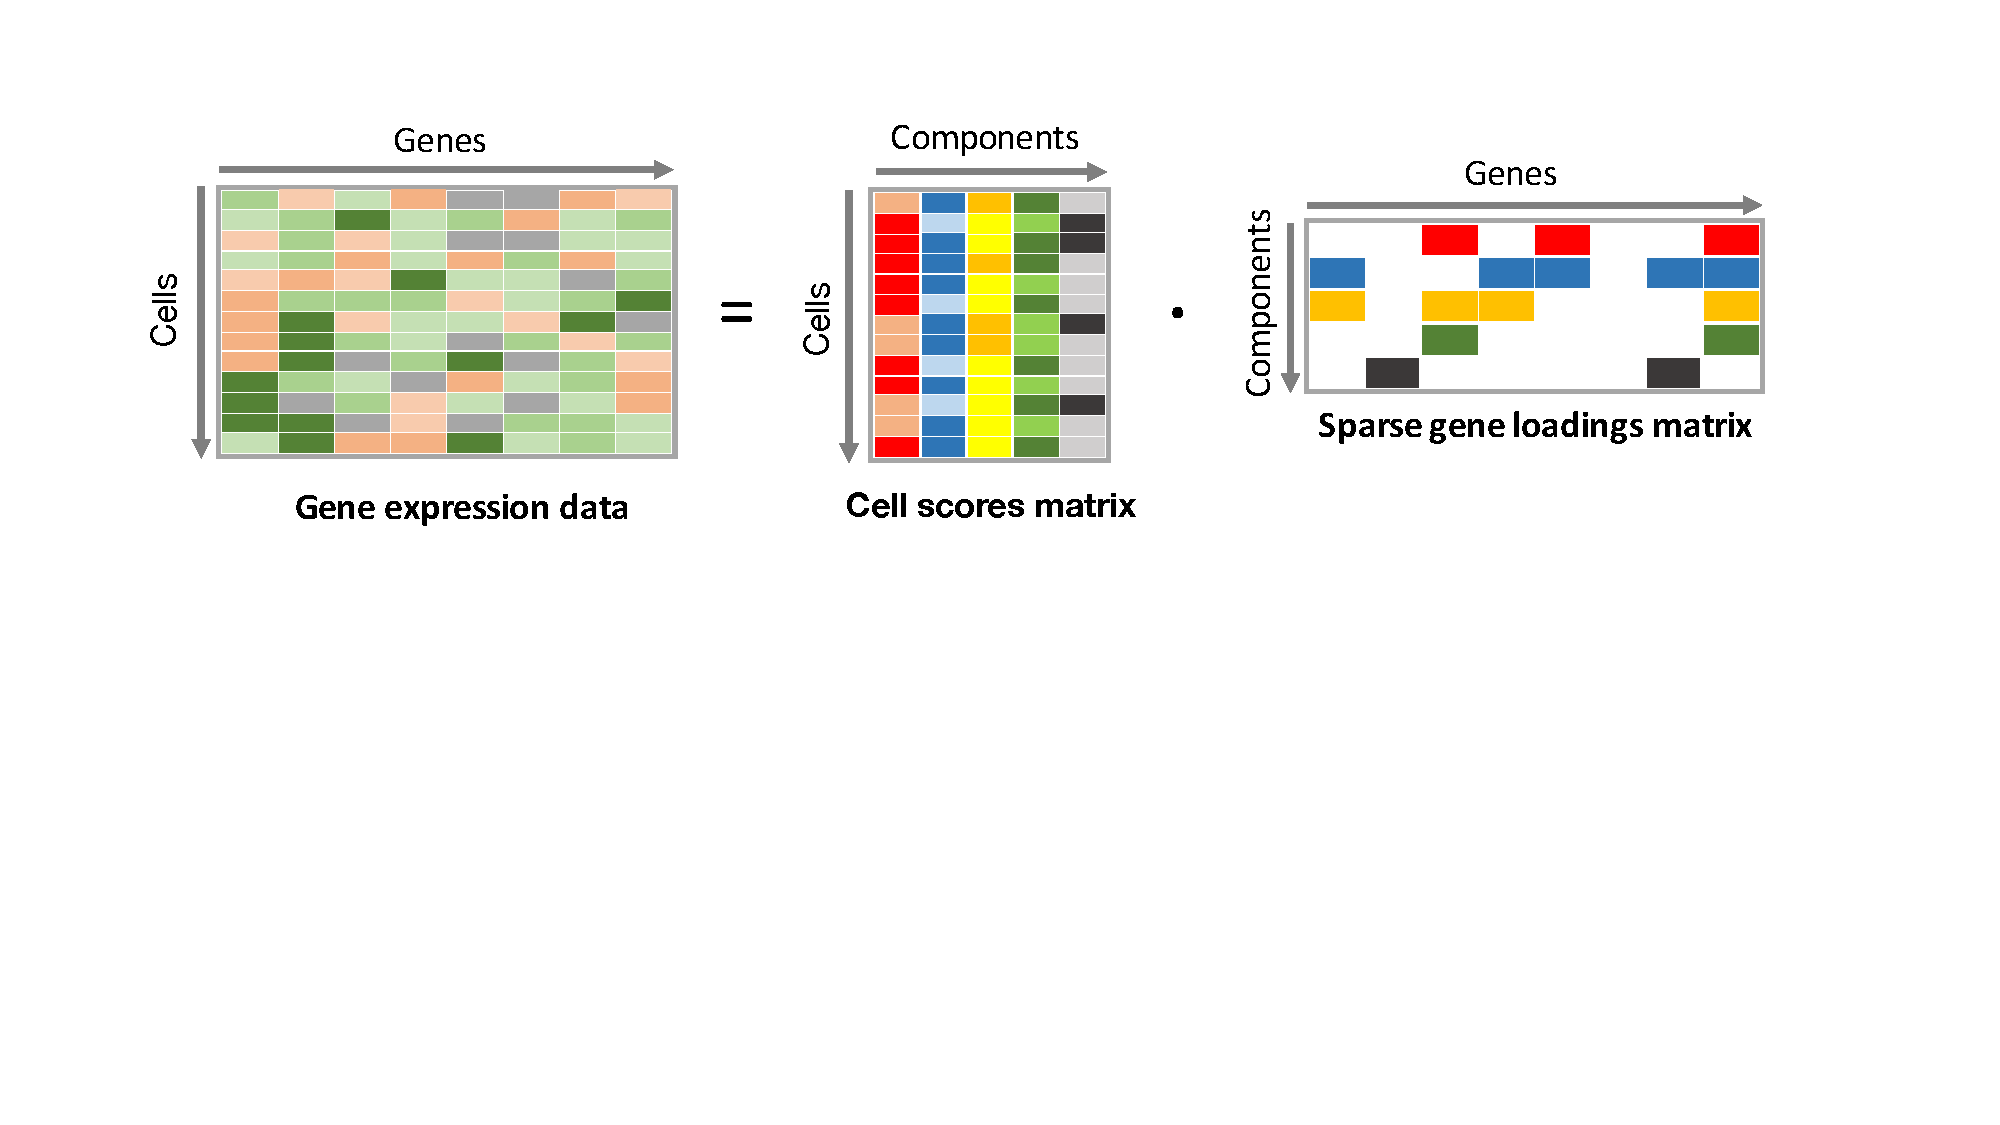
\includegraphics[width=\textwidth]{figures/intro/matrix_decomp_cells.pdf}
	\caption[SDA Matrix Factorisation]{Schematic of the SDA matrix factorisation. From \parencite{Hore2015Latent}}
	\label{fig:SDAfactorisation}
\end{figure}

Sparse decomposition of Arrays (SDA) is a sparse Bayesian factor analysis method, originally developed for decomposing a tensor of multi-tissue bulk RNAseq data, but can also be used in a group factor decomposition mode or to decompose a single 2D matrix (figure \ref{fig:SDAfactorisation}) \parencite{Hore2015Latent, Hore2016Tensor}.
The full model for the single matrix decomposition is given in equation \ref{eq:SDA} and in figure \ref{fig:SDAmodel}.

\begin{equation}
\begin{aligned}
y_{n l} &= \sum_{c=1}^{C} a_{n c} x_{c l}+\epsilon_{n l} \\
P(\mathcal{Y} | \theta) &=\prod_{l} \mathcal{N}_{N}\left(\mathbf{y}_{l} | \sum_{c} \mathbf{a}_{\cdot c} x_{c l}, \lambda_{l}^{-1} I_{N}\right) \\ 
P\left(a_{n c}\right) &=\mathcal{N}\left(a_{n c} | 0,1\right) \\
x_{c l} &= w_{c l} s_{c l} \\
P\left(w_{c l} | \beta_{c}\right) &=\mathcal{N}\left(w_{c l} | 0, \beta_{c}^{-1}\right) \\
P\left(\beta_{c}\right) &=\mathcal{G}\left(\beta_{c} | e, f\right) \\ 
P\left(s_{c l} | \psi_{c l}, \phi_{c l}\right) &=\mathcal{B} \text{ernoulli}\left(s_{c l} | p_{c l}\right) \\ 
p_{c l} &= \psi_{c l} \phi_{c l} \\
P\left(\psi_{c l}\right) &=\mathcal{B} \operatorname{eta}\left(\psi_{c l} | g, h\right) \\
P\left(\phi_{c l} | \rho_{c}\right) &=\mathcal{B} \text{ernoulli}\left(\phi_{c l} | \rho_{c}\right) \\
P\left(\rho_{c}\right) &=\mathcal{B} \operatorname{eta}\left(\rho_{c} | r, z\right) \\
P\left(\lambda_{l}\right) &=\mathcal{G}\left(\lambda_{l} | u, v\right) 
\label{eq:SDA}
\end{aligned}
\end{equation}

\begin{figure}[H]
	\centering
	\includegraphics[width=\textwidth]{figures/intro/SDA.pdf}
	\caption[SDA Model]{Schematic of the SDA Hierarchical Bayesian Model}
	\label{fig:SDAmodel}
\end{figure}

$\mathcal{Y}$ is an $N$ by $L$ matrix of cells by genes, $\mathcal{A}$ is a matrix of $N$ cells by $C$ components, and $\mathcal{X}$ is a matrix of $C$ components by $L$ genes, and $\mathcal{E}$ is an $N$ by $L$ matrix of independent Gaussian noise.

A key feature of this model is the element wise sparsity of the gene loadings which eases interpretation of the model, forms a kind of regularisation, and prevents the solution from being rotationally invariant.
Moreover this reflects a prior that generally only a subset of genes should be involved in any one biological process.
This sparsity is achieved by using a spike and slab prior which is a mixture of a point mass at 0 (spike) and a normal distribution (slab).
The slab $w$ has a precision of $\beta_{c}$ which has a Gamma prior with hyper-parameters $e = 10^{-6}$ and $f = 10^{-6}$ (diffuse).
The spike $s$ is modelled as a Bernoulli distribution with probability parameter $p_{cl}$ representing the probability of an individual gene loading being non-zero.
The prior on this parameter is itself a spike and slab with the slab $\psi_{c l}$ having a Beta prior with hyper-parameters $g=0$ and $h=0$ (a prior with half mass at 0 and half at 1).
The spike $\phi_{c l}$ again has a Bernoulli prior with parameter $\rho_{c}$ which also has a Beta prior with hyper-parameters $r=1$ and $z=1$ (flat).
This hierarchical structure encourages sparsity as when $\rho_{c}$ is close to 0 the prior on the main spike and slab will be dominated by the spike.
The factored spike and slab is equivalent to the pure mixture as in equation \ref{eq:SSMix} but aids inference.

\begin{equation}
P\left(x_{c l} | p_{c l}, \beta_{c}\right)=p_{c l} \mathcal{N}\left(x_{c l} | 0, \beta_{c}^{-1}\right)+\left(1-p_{c l}\right) \delta_{0}\left(x_{c l}\right)
\label{eq:SSMix}
\end{equation}

Each cell score has a standard normal prior.
Due to scaling indeterminacy (for example the cell scores could be multiplied by two and gene loadings halved with equivalent fit), the variances are set to 1 with any scaling occurring in the $\beta_{c}$ of the gene loadings.
The sign of the components is also unidentifiable, in addition to permutation of the components.

Each gene has a noise precision parameter $\lambda_{l}$ with a Gamma prior where the hyper-parameters are set to $u = 10^{-6}$ and $v = 10^{-6}$ resulting in a diffuse prior. 

The model is fit using variational Bayes as described in \parencite{Hore2015Latent, Hore2016Tensor}.
As variational Bayes underestimates variances, the mean of the posterior distributions are used rather than the distributions themselves \parencite{Jaakkola2000Bayesian}.
Sparse factor analyses using the spike and slab prior have also previously been used \parencite{West2003Bayesian, Lucas2006Sparse}.
The complexity is $\mathcal{O}(NLC^2)$ and the number of components must be chosen ahead of time, although in practice SDA can set entire components to zero if too many components are used \parencite{Hore2015Latent, Hore2016Tensor}.

%\begin{figure}[H]
%	\centering
%	\includegraphics[width=\textwidth]{figures/intro/pseudotime_methods.png}
%	\caption[Pseudotime Methods]{Comparison of pseudotime inference methods, reproduced from~\cite{Cannoodt2016Computational}}
%	\label{fig:pseudotime_methods}
%\end{figure}


% Similar aims (delineating lineage hierarchies and transcriptional networks) have been achieved using single cell RNA-seq in tissues other than testis, highlighting the feasibility of this study~\cite{Trapnell2014Dynamics,Treutlein2014Reconstructing,DurruthyDurruthy2014Reconstruction,Moignard2013Characterization,Stegle2015Computational}.

%\subsection{Principal Components Analysis}

%\subsection{Sparsity}

%Frequentist
%Bayesian

\begin{savequote}[8cm]
The association of paternal and maternal chromosomes in pairs and their subsequent separation during the reducing division as indicated above may constitute the physical basis of the Mendelian law of heredity.
   \qauthor{--- \cite{Sutton1902morphology}}
\end{savequote}

\chapter{\label{ch:2-SDA} Single Cell Transcriptomics}

\minitoc

\section{Experimental Data Generation}

The experimental work in this chapter was performed by Min Jung and colleges in Don Conrad's group at the University of Washington, St Louis.

The samples generated are as follows:

\begin{itemize}
	\item 11 wild type C57BL/6 mice
	\item 3 FACS samples (primary spermatocyte , secondary spermatocyte, and spermatid) from a 12th wild type
%	\item 1 C57BL/6 mouse
	\item 1 sample of FACS sorted spermatogonial cells from 5 wild type C57BL/6 litter mates with GFP tagged Pou5f1 (B6;CBA-Tg(Pou5f1-EGFP)2Mnn/J, \cite{Szabo2002Allelespecific})
\end{itemize}

In addition to wild type mice four different mutant mice were included:
\begin{itemize}
	\item 6 \textit{Mlh3\textsuperscript{-/-}} mice (B6.129-Mlh3\textsuperscript{tm1Lpkn}/J, \cite{Lipkin2002Meiotic})
	\item 2 \textit{Hormad1\textsuperscript{-/-}} mice (B6;129S7-Hormad1\textsuperscript{tm1Rajk}/Mmjax, \cite{Shin2010Hormad1})
	\item 2 \textit{Cul4a\textsuperscript{-/-}} mice (B6;129-Cul4a\textsuperscript{-/-}, \cite{Yin2011E3})
	\item 2 CNP eGFP BAC TRAP (knockin) C57BL/6 mice (Joseph Dougherty).
\end{itemize}

The cells were dissociated by two methods: enzymatic for the first two wild type mice and the spermatogonia, and mechanical for all other samples \cite{Lima2017Standardized,Jung2019Unified}. The cells where then encapsulated using the DropSeq protocol \cite{Macosko2015Highly} as described in \cite{Jung2019Unified}.


\section{Data Processing and QC}

The samples were sequenced on either Illumina HiSeq2500 or MiSeq. Reads were mapped to the mouse using DropSeq tools provided by Macosko lab (using STAR aligner and GRCm38 release 90).

The resulting cell-gene count matrices were merged (54,251 cells and 38,317 genes) and processed through a series of quality control and normalization steps:

Genes with a UMI count of less than 5 or being expressed in fewer than 5 cells were removed.

Cells meeting the following criteria were removed:
\begin{itemize}
\item UMI count of less than 200
\item Fewer than 100 genes expressed
\item Log UMI count more than 1 standard deviation below the mean for that experiment
\item Log number of genes expressed was more than 1 standard deviation below the mean for that experiment
\end{itemize}

A tSNE dimensionality reduction of the filtered data revealed an amorphous homogeneous group of cells with low library size, high mitochondrial gene expression and often co-expressed genes from both early and late spermatogenesis suggesting poor quality and/or doublet cells. This group of cell was therefore removed before further analysis in addition to any cells with a normalised \textit{mt-Rnr-2} expression of greater than 2 suggestive of lysed cells \cite{Ilicic2016Classification}. These filters resulted in 20,322 cells and 28,893 genes remaining.

Genes in the lower third of expression means were then removed and cells were normalized by square root transformation of total transcript counts per cell and genes were normalized to unit variance. All expression values were capped to maximum of 10. This results in a final matrix of 20,322 cells by 19,262 genes with a sparsity of 93.8\% and a median UMI count of 1,312 per cell.


\section{SDA}

When performing a dimensionality reduction such as matrix factorisation we must somehow determine the number of latent components. Too low and we may miss some real components, too high and we may find spurious components due to overfitting. One way the method can overfit is by assigning a whole component to an individual cell, which we observed (Fig \ref{fig:single_cell_component}). We found when increasing the number of components from 50 to, 75, 100, 200 and 500 we got more of these single cell components rather than new normal components. With 50 components we had five individual cell components (1,4,8,14, and 46 - fig \ref{fig:SDA_diagnostics}) which we judged to be an acceptable balance between over and underfitting. We also ran SDA with five different random seeds to confirm stability of the results with different initialisations.


\begin{figure}[H]
	\centering
	\includegraphics[width=\textwidth]{figures/single_cell_component.pdf}
	\caption{Component 4 is represents a single cell.
		\textbf{(A)} Cell scores for component 4 ordered by value.
		\textbf{(B)} Gene loadings for component 4.
		\textbf{(C)} Predicted expression using only component 4 vs Raw Normalised Gene Expression. Pearson's correlation is quoted (equal to correlation with the gene loadings) . All of the genes with high expression in this cell have a high gene loading in this component.
		\textbf{(D)} As in C but for the cell with the second highest association. The correlation is much lower. 
		\textbf{(E)} As in C but using all components except 4. The correlation is less than C especially for highly expressed genes.
		\textbf{(F)} As in C but using all components for the prediction.  This is the sum of C and E
	}
	\label{fig:single_cell_component}
\end{figure}

By inspecting the change in free energy as well as the change in fraction of gene loadings with PIP < 0.5 we can confirm that the algorithm had converged within the 10,000 iterations for which it was run \ref{fig:SDA_diagnostics}. In addition the results are almost identical after 1,000 iterations (fig \ref{fig:10k}. Mean runtime for 10,000 iterations was 41.8 hours on a single core of Intel Xeon E5-2667 v4. The computational complexity of SDA scales with $NLC^2$ where N=number of cells, L=number of genes, and C=number of components. We acknowledge SDA is not the fastest way to analyse single cell RNA-seq data, however we prefer additional insight over gains in speed which for datasets of similar size to ours will be small relative to the time for data generation and analysis overall. As expected in line with previous reports from \cite{Hore2016Tensor} the PIPs have a bimodal distribution \ref{fig:SDA_diagnostics}.

\begin{figure}[H]
	\centering
	\includegraphics[width=\textwidth]{figures/SDA_diagnostics.pdf}
	\caption{Checking convergence of SDA.
		\textbf{(A)} Change in free energy is often 0 by the 10,000th iteration.
		\textbf{(B)} Change in fraction of PIP <0.5 is less than 0.005\%
		\textbf{(C)} Distribution of maximum scores and loadings for each component.
		\textbf{(D)} Distribution of PIPs across all components, showing expected bimodal distribution.}
	\label{fig:SDA_diagnostics}
\end{figure}

\begin{figure}[H]
	\centering
	\includegraphics[width=\textwidth]{figures/1k_vs_10k.pdf}
	\caption{Correlation of gene loadings between set inferrred using 1,000 iterations vs those using 10,000 iterations.}
	\label{fig:10k}
\end{figure}


The gene loadings are sparse with 79.8\% of the gene loadings having a PIP of less than 0.5 (fig \ref{fig:SDA}B,C). These genes have a tight distribution of loadings around 0 with a maximum absolute loading of 0.011 and 99\% of the loadings lying within the range (-0.0033, 0.0036). Of the gene loadings with a PIP of greater than 0.5 the maximum absolute loading is 1.31 and the mean is 0.062.


\section{Low Dimensional Visualisation}

\begin{figure}[H]
	\centering
	\includegraphics[width=\textwidth]{figures/tsne_random_seeds.png}
	\caption{
		\textbf{(A-C)} To quantify our uncertainty in the t-SNE embedding, we performed multiple t-SNE analyses with different random seeds. The cells are coloured by the same pseudotime values used throughout. Somatic cells are coloured gray. t-SNE coordinates are rotated about the origin to aid comparison.
		\textbf{(D)} We also performed dimensionality reduction using UMAP and confirmed that it gave a pseudotime embedding consistent with t-SNE. Cells are again coloured using the same psueodtime values as A-C}
	\label{fig:tSNEseeds}
\end{figure}

Despite reducing the dimensionality of the original dataset from 19,262 to 50 this is still too high to visualise the overall structure of the data. This can be achieved by performing a second non-linear reduction such as tSNE or UMAP (normally PCA is the linear reduction) \cite{Maaten2008Visualizing, McInnes2018UMAPa, Becht2018Dimensionality}. We find a horseshoe like effect often found when reducing datasets with an underlying 1 dimensional structure \cite{Novembre2008Interpreting, Podani2002RESEMBLANCE} (Fig \ref{fig:tSNEseeds}). By looking at genes with known expression patterns from the literature we can induce that in this case that the linear structure is developmental time of spermatogenesis and that the clusters in the centre are somatic cells (Fig \ref{fig:Marker_Genes}).


\begin{figure}[H]
	\centering
	\includegraphics[width=\textwidth]{figures/Marker_Genes.pdf}
	\caption{Imputed expression for genes with a range of expression patterns across cells}
	\label{fig:Marker_Genes}
\end{figure}

To generate a pseudo-timeline we used a similar approach to that implemented in SCUBA \cite{Marco2014Bifurcation}. We iteratively fit a principal curve through the t-SNE plot with increasing degrees of freedom from 4 to 9 using the curve from the previous run as the starting point \cite{Hastie1989Principal}. Each cell was then assigned to the closest position on this curve. Somatic cells and the Hormad1 X-activated cells (component 38 score >3) were excluded during pseudotime construction but the \textit{Hormad1\textsuperscript{-/-}} X-activated cells were given pseudotimes post-hoc. Somatic cells were defined by thresholding the cell scores of somatic components (if the absolute cell score of a given cell passed any of the following component thresholds 26, 11, 3, 32, 45, 24 > 2; 37 > 1.5; 40 > 1; or mt-Rnr2 expression >3).

The temporal order of components was determined by using a weighted mean of the pseudotime values, where the weights are the cell scores of the component. In addition, only those cells with an absolute cell score of greater than two contribute to the mean.

Although the model used for inference is symmetric for positive/negative gene weightings, many identified components showed strong biases towards positive or negative weights, consistent with expectations for identifying a group of co-activated (or co-repressed) genes (e.g. figure \ref{fig:SDA}E). Likewise, the cell loadings of each component frequently highlight specific cellular subsets that localize in t-SNE space and pseudotime (Figure \ref{fig:SDA} and \ref{fig:Cell_Scores})

\begin{figure}[H]
	\centering
	\includegraphics[width=\textwidth]{figures/SDA.pdf}
	\caption{
		\textbf{(A)} Schematic illustrating SDA
		\textbf{(B)} Density of gene loadings over all components with loadings separated into genes with PIPs > 0.5 (20\%) versus <0.5, indicating the sparsity of resulting gene loadings. PIP = Posterior Inclusion Probability that a gene loading is not equal to zero (i.e. not in the spike).
		\textbf{(C)} For each method, the fraction of all absolute gene loadings exceeding a ‘no loading’ sparsity threshold is shown, normalized by the maximum absolute loading across all components for that method. 
		\textbf{(D)} t-SNE projection of the cell scores from SDA. Each point it a cell, each coloured by their loading in component 5. Black arrow: the principle curve fit to the germ cell data, corresponding to the developmental ordering of each cell progressing through spermatogenesis. The coloured segmented line shows broad staging of spermatogenesis.
		\textbf{(E)} Gene loadings for component 5, plotted along the genome. Red genes: GWAS hits for human recombination rate.
		\textbf{(F)} Enrichment for GWAS hits of human recombination rate for all components. OR: Odds Ratio. P value by FET (main text). Positive (P) and negative (N) loadings are tested separately. For one-sided components (cell score range ratio >5) the minor side is omitted. Red horizontal line: p=0.05 after Bonferroni correction for multiple testing.
	}
	\label{fig:SDA}
\end{figure}

We can perform the same dimensionality reduction on the transposed cell scores or gene loadings to see how the components relate to each other (Fig \ref{fig:tSNE_Components}). We find 7 major clusters of components and with hindsight these correspond to: 1) Spermatogonia, 2) Leptotene/Zygotene 3) Pachytene 4) Round Spermatid (Acrosomal) 5) Spermiogenesis 6) Somatic and 7) Somatic (Sertoli). We can see that our manual labelling of the components is consistent with the clusters.

\begin{figure}[H]
	\centering
	\includegraphics[width=\textwidth]{figures/tSNE_Components.pdf}
	\caption{A low dimensional representation of the components shows 7 clusters.}
	\label{fig:tSNE_Components}
\end{figure}

Visualisation of components through pseudotime shows that transcription during spermatogenesis can be represented as a series of overlapping components, each varying with different timescales (Fig \ref{fig:SDA_overlapping} A\&B). Furthermore, these components are comprised of distinct gene sets enriched for distinct biological processes (Fig \ref{fig:SDA_overlapping} C\&D).

\begin{figure}[H]
	\centering
	\includegraphics[width=\textwidth]{figures/SDA_Overlaping.pdf}
	\caption{
		\textbf{(A)} For five example components, the cell scores for each cell are plotted through pseudotime, showing overlapping dynamic component activity. Component signs were chosen to be mainly positive (components have arbitrary sign). Color mappings as in panel B.
		\textbf{(B)} Stacked bar plot of cell component loadings for 14 germ components sorted by cell pseudotime. Each column corresponds to an individual cell and the total positive component loadings for each are normalized to one after flipping components to be mainly positive.
		\textbf{(C)} Shown are the top 10 gene loadings for each of the components in (B) represented as a heatmap. Most genes have strong loading on only one component.
		\textbf{(D)} Gene ontology enrichment analysis for biological processes in the top 250 genes for each component }
	\label{fig:SDA_overlapping}
\end{figure}



\section{Imputation}

In addition to identifying soft clusters and their marker genes, In the process of fitting the SDA model we have also effectively imputed the very sparse and noisy data. Multiplying out the cell scores and gene loadings matrix generates a matrix of the same dimensions as the original data but populated with the models predicted values. SDA imputation is able to estimate expression of individual genes even when in many cells zero reads are observed (Fig \ref{fig:imputation}A). In addition SDA expression estimates have fewer outlying high values outside the genes main expression window. The destructive nature of the single cell RNAseq protocol means that it is not possible to determine the true expression vector for an individual cell. In order to determine if imputation is actually improving our estimates we use cross-validation. Specifically, we randomly assign each read to either a training or test set, predict gene expression based on the training set (using SDA, or another method for example the dedicated imputation method MAGIC from \cite{vanDijk2018Recovering}) and then evaluate our ability to rank gene expression using the test set (methods). SDA imputation outperforms approaches using the raw data for essentially all cells in the test data (Fig \ref{fig:imputation}B\&C).

While providing the most sparse representation (Fig \label{fig:SDA}C), SDA still imputes equally well, compared to other matrix factorizations and MAGIC \parencite{vanDijk2018Recovering} (Fig \ref{fig:imputation}C \& \ref{fig:imputation_supp}A). Some cells gain more from imputation than others, the cells that gain the most are those with low library size (Fig \ref{fig:imputation_supp}C).

Furthermore, by comparing the genes with the lowest correlation between NNMF and SDA imputed expression, we found that SDA provides additional biological insights for the same number of components (Fig \ref{fig:imputation}D,E,F \& \ref{fig:imputation_supp}B). SDA infers multiple components for undifferentiated spermatogonia whereas NNMF only infers a single component resulting in imputed expression of \textit{Gfra1} and \textit{Lin28a} in the same cells (Fig \ref{fig:imputation}D and Figure \ref{fig:imputation_supp}B - no correlation for SDA component 50 \textit{Gfra1} Stem Cells). NNMF predicts a peak in the expression of X linked gene \textit{Rhox2h} even in WT cells, in which X chromosome activation due to Hormad1 KO does not occur suggesting underfitting of the data with 50 components (Fig \ref{fig:imputation}E). NNMF does not predict high expression of the adaptive immune cell marker \textit{Cd3g} (T-cell surface glycoprotein CD3 gamma chain), and when it predicts any expression it increases linearly with the innate immune cell marker \textit{Csf1r} (Macrophage Colony-Stimulating Factor 1 Receptor, or \textit{Cd115}) (Fig \ref{fig:imputation}F). In contrast SDA correctly predicts that \textit{Cd3g} and \textit{Csf1r} are not coexpressed in the same cells (See also \ref{fig:imputation_supp}B, no correlation for the SDA component 3 Lymphocytes).

In addition to obviating the need for further clustering and differential expression analyses, an advantage of using matrix factorization for imputation is the much smaller memory footprint required to store the results: on our dataset MAGIC data is 2.9 Gb whereas the SDA matrices are just 18 Mb (12.6 Mb when loadings with PIP <0.5 are set to 0).


\begin{figure}[H]
	\centering
	\includegraphics[width=\textwidth]{figures/imputation&NNMF.pdf}
	\caption{
		\textbf{(A)} For seven genes expressed at various stages of spermatogenesis unimputed normalised gene expression is shown alongside SDA imputed expression.
		\textbf{(B)} Prediction accuracy of seven predictors of gene expression trained on test data for an example individual cell. ‘Unimputed’ uses the training data directly, ‘Mean Cell’ uses the mean across all cells, matrix factorisation approaches SDA, PCA, ICA, NNMF, and a dedicated imputation approach, MAGIC.
		\textbf{(C)} Comparison of AUCs (Area under the curve) for all cells using various methods (same colour scheme as part B).
		\textbf{(D)} Zoomed versions of the t-SNE projection (with full t-SNE for context): cells are coloured by expression using a three channel ternary colour scheme with the amount of blue, green, red representing the respective expression levels of \textit{Lin28a}, \textit{Nanos1}, and \textit{Gfra1}.
		\textbf{(E)} Imputed expression of X chromosomal gene \textit{Rhox2h} from either the SDA or NNMF decomposition, split into cells we know to be either WT or \textit{Hormad1\textsuperscript{-/-}} genotype.
		\textbf{(F)} Imputed expression of \textit{Cd3g} and \textit{Csf1r} for both NNMF and SDA.}
	\label{fig:imputation}
\end{figure}

\begin{figure}[H]
	\centering
	\includegraphics[width=\textwidth]{figures/Imputation_Supp.pdf}
	\caption{
		\textbf{(A)} Imputed expression of an example gene (\textit{Smok2b}) for different methods, to illustrate the similar predictions as shown in Figure \ref{fig:imputation}B and \ref{fig:imputation}C.
		\textbf{(B)} Overall, NNMF infers similar components to SDA. The heatmap shows Pearson correlations between different pairs of gene loading vectors from SDA and NNMF (with procrustes rotation applied, Materials and methods).
		\textbf{(C)} The fold improvement in AUC when comparing SDA imputation to the unimputed data, plotted as a function of cell library size.
	}
	\label{fig:imputation_supp}
\end{figure}

\section{Mutant Genotypes}

Given we combined both wild-type and mutant cells in our analysis it is important to check that the components representing wild type processes are not unduly affected by this mixing. In order to quantify the robustness of our conclusions to this decision to combine mutant and wild-type strains, we performed a separate SDA analysis using just wild-type cells (the ‘WT’ analysis) and compared the results.

Factor analyses naturally have a degree of unidentifiability, whereas in SDA the sparsity prior helps to make the model identifiable across different seeds. For different data however the gene loadings matrix may be a rotated version in which components are linearly split or combined. A procrustean rotation can align two matrices (here gene loadings) onto an equivalent set of axes. Therefore, for fair comparison across SDA runs with different datasets, we compared the correlation of the gene loadings after procrustan rotation which tells us if the components inferred are effectively the same.

We found that most components generated from an SDA analysis of only wild-type data were also observed in the joint analysis of wild-type and mutant data. The most important WT components (those with high total cell score) have high correlations with components in the mixed SDA run (fig \ref{WT_vs_Mixed}). Some components such as Mix38 X activation are not represented in the WT decomposition because they represent mutant-specific processes. Other components such as Mix44 Leptotene-Zygotene do not appear as these cells are numerous only in mutant samples which lack the more abundant later stages of cells.

By visualising the rotation matrix from the procrustean analysis we can see which components have been rotated. For example Mix component 17 spermiogenesis is a linear combination of WT component 46 and 7 (fig \ref{fig:WT_Mix_Rotation}). We can also visualise the correlations directly as in figure \ref{fig:WT_Mix_Correlation}.

\begin{figure}[H]
	\centering
	\includegraphics[width=\textwidth]{figures/correlation_matrix_rotated.pdf}
	\caption{Here we show as a heatmap the pearson correlation of component gene loadings between a procrustean rotation of the WT gene loadings and the Mixed SDA gene loadings. The ‘sum abs cell score’ annotation shows the sum of the absolute cell scores for that component (larger number indicates a more important component). The ‘max cell score’ annotation indicates the maximum cell score for each component (a larger maximum indicates overfitting to a single/small number of cells).}
	\label{fig:WT_vs_Mixed}
\end{figure}

\begin{figure}[H]
	\centering
	\includegraphics[width=\textwidth]{figures/rotation_matrix_sparseNEW.pdf}
	\caption{This heatmap shows the procrustean rotation matrix (with absolute values < 0.35 rounded down to 0).}
	\label{fig:WT_Mix_Rotation}
\end{figure}

\begin{figure}[H]
	\centering
	\includegraphics[width=\textwidth]{figures/UdifSpg_gene_scatterplot.pdf}
	\caption{An example scatterplot comparing the gene loadings for one cognate SDA component (C31) between WT and Mixed SDA runs. The correlation is high.}
	\label{fig:WT_Mix_Correlation}
\end{figure}


\section{Non Meiotic Components}

Given we combined multiple experimental batches it's important to correct for batch effects and SDA provides a simple approach as some inferred components will capture these effects and can be removed.

Component 22 gene loadings are highly enriched in ribosomal proteins (50 of the top 100 loadings are non pseudogene ribosomal genes - of which there are 99, Fig \ref{fig:NonMeiotic}A). However unlike ribosomal component 43, the cell scores for component 22 are associated with whether the sequencing was done on MiSeq or HiSeq Illumina machines and so this component is likely a batch effect (Fig \ref{fig:NonMeiotic}B).

Component 12 has high cell loadings for \textit{Hormad1\textsuperscript{-/-}} cells, but these loadings are largely positive for the first two libraries, and negative for the last library (Fig \ref{fig:NonMeiotic}C,D).

Component 9 contains 41 out of 57 of the respiratory complex I, III, and IV genes (complex II is an alternative pathway) Fig \ref{fig:NonMeiotic}E,F (p = 7.4x10-53, OR = 104 [95\% CI: 62.1,Inf] FET). It's not clear whether this component reflects real meiotic biology or potentially reflects cell stress induced by experimental processing (still a real biological process but not one that exists in vivo).

\begin{figure}[H]
	\centering
	\includegraphics[width=\textwidth]{figures/NonMeiotic_Components.pdf}
	\caption{
		\textbf{(A \& B)} Gene loadings and cell scores for component 22.
		\textbf{(C and D)} Gene loadings and cell scores for component 12.
		\textbf{(E)} Gene loadings for component 9. Genes that are (non-assembly) components of the electron transport chain proton pump genes are highlighted in red. This gene set is defined by the genes that match the regex ‘Uqc|Cox|Ndu’. Pseudogenes, and genes with ‘assembly|like’ in their name were excluded.
		\textbf{(F)} Enrichment of genes that are (non-assembly) components of the electron transport chain proton pump genes in the top 500 genes from each component.
	}
	\label{fig:NonMeiotic}
\end{figure}


\section{Components}

Assigning a cytologically defined stage to each component requires considerable manual work due to lack of any high resolution data. There are a number of issues that complicate assignment. Firstly as we have seen components activities are gradual and so there may be no well defined set of cells or start and end to a component. Components can be mixed sign (positive/negative) and one sign may be active in a different stage to the other. Stages themselves are not well defined in the literature with multiple definitions being used by different groups. Due to translational regulation the transcription of genes may not correspond to the detection of the protein, hence using commonly performed antibody based immunofluorescence can be misleading and if available mRNA detection methods should be used for reference. In addition any literature references from human, or even rat, can have different expression patterns than mouse and so this evidence must be used with caution. Nonetheless using a combination of evidence types from multiple genes for each component we were able to assign almost all components to a stage(s) or cell type(s).


\begin{figure}[H]
	\centering
	\includegraphics[width=\textwidth]{figures/Cell_Scores.png}
	\caption{}
	\label{fig:Cell_Scores}
\end{figure}




\subsection{Telocytes}
Recently telocytes were discovered to be present in the mammalian (human) testis \parencite{Marini2018Reappraising, Kuroda2004Distribution}. We find one component (\#32) matching the known combination of markers for telocytes (\textit{Cd34} and \textit{Pdgfra} positive, \textit{Kit}, \textit{Pecam} and \textit{Acta2}/\textalpha-SMA negative) in addition to many other genes specific to this cluster (\textit{Dcn}, \textit{Col1a2}, \textit{Col1a2}, \textit{Col3a1}, \textit{Col6a1}, \textit{Col4a4}, \textit{Col4a1}, \textit{Col1a1}, \textit{Lamb1}, \textit{Lama2}, \textit{Lamb2}, \textit{Gsn}, \textit{Adamts5}, \textit{Mgp}) representing potential novel markers for this cell type in the testis. This component is highly enriched for the GO term "extracellular matrix organization" (p=4.3e-16, OR=10.3). Their expression pattern matches what was described as an unknown mesenchymal cell population by \cite{Green2018Comprehensive} with expression of \textit{Tcf21}, \textit{Arx}, \textit{Vim}, and \textit{Col1A1}, but not \textit{Acta2} (\textalpha-SMA), or \textit{Cyp17a1}.


\subsection{Leydig Cells}
Component 40 broadly marks all Leydig cells and has high gene loadings for all the major genes required for testosterone production including \textit{Star}, \textit{Cyp11a1}, \textit{Hsd3b}, \textit{Cyp17a1}, and \textit{Hsd17b} \ref{fig:testoterone} \cite{Stojkov2013Orally} in addition to other markers of Leydig cells including \textit{Insl3} and \textit{Ptgds} \parencite{Balvers1998RelaxinLike, Baker2001Expression}. This component is most highly enriched for the GO term "steroid metabolic process" (p=5.3e-23, OR=11.3)

Component 26 splits Leydig cells into two main groups, distinguished by the expression of \textit{Fabp3}, \textit{Gstm1}, \textit{Gsta3}, and \textit{Ass1}.

Component 24 is a subtype of the \textit{Fabp3} expressing C26 positive cells, which has high expression of \textit{Gstm3}, \textit{Mt3}, \textit{Thrsp}, and \textit{Jak3}, but also a number of pseudogene versions of genes that are normally expressed leydig genes: \textit{Gstm2-ps1}, \textit{Gm6665} (another \textit{Gstm2} pseudogene), \textit{Fabp3-ps1}, \textit{Gm8834} (\textit{Gstm3} pseudogene), \textit{Gm5096} (\textit{Bhmt} pseudogene), \textit{Gm6977} (\textit{Fth1} pseudogene), \textit{Gm7049} (\textit{Me1} pseudogene).

Component 19 marks cells in both major groups and is distinguished by high expression of a group endopeptidases encoded in a 300kb locus on chromosome 7 including \textit{Klk1}, \textit{Klk1b1}, \textit{Klk1b21}, \textit{Klk1b22}, \textit{Klk1b24} and \textit{Klk1b27}. Some of these genes are known to be specifically expressed in Leydig cells and may be involved in remodelling of the extracellular matrix \parencite{Sanz2013RiboTag, Matsui2000Cloning, Matsui2001Mouse, Matsui2005Characterization}.

\subsection{Sertoli Cells}

Component 37 is active in cells expressing \textit{Wipf3} (aka CR16) and \textit{Ncoa2} (aka TIF2) both of which are required for fertility and have Sertoli restricted expression \cite{Suetsugu2007Malespecific, Gehin2002Function}). In addition \textit{Nxf3} is specifically expressed in Sertoli cells but not required for spermatogenesis \cite{Zhou2011Nxf3}.

%45

%16

\subsection{Macrophages}
We find one component (\#11) representing macrophage cells. This component has high loadings for \textit{Csf1r} (macrophage colony-stimulating factor receptor, aka CD115), \textit{Cd163} (macrophage scavenger receptor), \textit{Cd68}, \textit{Adgre1} (aka F4/80), \textit{Itgam} (aka CD11b), \textit{Mrc1}, \textit{Cx3cr1}, \textit{Fcgr3}, and the complement genes \textit{C1qa}, \textit{C1qb}, and \textit{C1qc}. \parencite{Mossadegh-Keller2017Developmental, Fabriek2005macrophage, Sasmono2012Generation}

Immunohistochemical staining of ADGRE1 found that macrophages were present within the tubule, which is typically regarded as immune privileged partly due to the blood-testis barrier formed by sertoli cell tight junctions \parencite{Fijak2006testis}. Macrophages have previously been reported within the adluminal compartment, although always in the context of testicular defects \parencite{Frungieri2002Number, Goluza2014Macrophages}.


\subsection{Lymphocytes}
Component 3 is highly enriched for genes involved in T cell activation (p=1.4e-19, OR=7.6) and has high loadings for (T-cell) lyphocyte genes including \textit{Ptprc} (aka CD45, leukocyte common antigen), \textit{Cd2} (aka T-cell surface antigen) \parencite{Murray2011Protective, Murphy2012Janeway}, \textit{Ms4a4b} (high protein expression in T and NK but not B cells \cite{Xu2010MS4a4B}), and the CD3 T-cell receptor complex genes: \textit{Cd3g}, \textit{Cd3d}, \textit{Cd3e}, \textit{Trbc2}, \textit{Trac} \parencite{Call2002Organizing}.


\subsection{Peritubular Myoid}
% 21??

Component 10 is active in a small number of cells, likely to be peritubular myoid cells due to co-expression of \textit{Cnn3}, \textit{Edn1} (Endothelin), \textit{Myh11} (Smooth muscle myosin heavy chain), and \textit{Acta2} (Smooth muscle actin) \parencite{Mayerhofer2013Human}. The most significant GO term is "muscle tissue development" (p=8.789135e-08, OR=4.97).





\subsection{Spermatogonia}

% Spermatogonia can are the most undifferentiated germ cells in the adult body. There are a number of different types which can be categorised according to the Oakberg scheme in mice \parencite{Oakberg1971Spermatogonial}. As are the most stem cell like, which divide into Apr, Aal4, Aal be \parencite{vanPelt1990Synchronization}

Five components correspond to processes in spermatogonia. Component 31 represents undifferentiated spermatogonia expressing \textit{Zbtb16} (aka \textit{Plzf}) \parencite{Buaas2004Plzf} and \textit{Foxo1} \parencite{Goertz2011Foxo1}, while component 50 splits these into two subpopulations one expressing, \textit{Gfra1} (shown to be expressed in a subset of As and required for As self renewal by acting as a co-receptor for GNDF \parencite{Meng2000Regulation,He2007Gfra1}) and \textit{Glis3} \parencite{Kang2016Transcription}, and the other \textit{Nanos3} \parencite{Suzuki2009heterogeneity}, \textit{Lin28a} \parencite{Zheng2009pluripotency} and \textit{Foxf1}. Component 7 likely represents A1-4 spermatogonia as they express c-Kit which is expressed in differentiated (not undifferentiated) spermatogonia \parencite{Manova1990Gonadal,Schrans-Stassen1999Differential} and is required for the A1 to Al divisions \parencite{Yoshinaga1991Role}. These cells also express \textit{Stra8} which is expressed from type A spermatogonia through to preleptotene cells in response to retinoic acid \parencite{Oulad-Abdelghani1996Characterization,Zhou2008Expressiona,Endo2015Periodic} and is required for premeiotic DNA replication \parencite{Baltus2006germ}. We find they these cells are also well marked by \textit{Plppr3}, \textit{Sertad4}, \textit{Met}, \textit{Jade2}, \textit{Nanos1}, \textit{Glis1} and \textit{Glis2}. Component 2 includes \textit{Ctcfl}, \textit{Pou4f1}, and \textit{Esx1} - likely representing intermediate and type B spermatogonia \parencite{Sleutels2012male, Budhram-Mahadeo2001closely, Maezawa2018Dynamic, Li1997Esx1, Branford1997Spx1}. Component 33 is broad component covering all the stages of spermatogonia.


\subsection{(pre)Leptotene \& Zygotene}

Component 5 includes many genes required for the creation and repair of meiotic double strand breaks. This includes \textit{Prdm9} itself; components of the meiotic cohesin complex \textit{Rad21l}, \textit{Smc1b}, \textit{Smc3}, \textit{Stag3} and \textit{Esco2} \parencite{Rankin2015Complex}; components of the telomere tethering complex \textit{Terb1}, \textit{Terb2}, \textit{Spdya}, and \textit{Sun1} \parencite{Ding2007SUN1, Tu2017Speedy, Wang2019meiotic}; genes involved in creating DSBs \textit{Mei1}, \textit{Ccdc36} (\textit{Iho1}), \textit{Spo11} partner \textit{Top6bl} (\textit{Gm960}), and regulator \textit{Atm} \parencite{Lukaszewicz2018Control, Reinholdt2005Mei1, Robert2016TopoVIBLike, Stanzione2016Meiotic, Vrielynck2016DNA}; proteins required for the creation and processing of the ssDNA intermediates and their regulators: \textit{Mcm8}, \textit{Dmc1}, \textit{Rad51}, \textit{Rad51ap2}, \textit{Atr}, \textit{Brca2}, \textit{Tex15}, \textit{Meilb2} (\textit{Hsf2bp}), \textit{Meiob}, and \textit{Spata22} \parencite{Brown2015Small, Brown2014DNA, Dai2017Meiotic, Kovalenko2006RAD51AP2, Lee2015MCM89, Martinez2016BRCA2, Pacheco2018ATR, Ribeiro2018MEIOB, Widger2018ATR, Xu2017Meiosisspecific, Yang2008Mouse, Zhang2019meiosisspecific}; class I crossover (ZMM group) proteins \textit{Shoc1} (\textit{Zip2} orthologue), \textit{Tex11} (\textit{Zip4} orthologue), \textit{Msh5}, \textit{Hfm1} (\textit{Mer3} orthologue) and regulator \textit{Brip1} (\textit{FancJ}) \parencite{Adelman2008ZIP4H, Guiraldelli2018SHOC1, Guiraldelli2013Mouse, Rakshambikai2013Structural, Sun2016FancJ}; as well as components of the synaptonemal complex \textit{Sycp1}, \textit{Sycp2}, \textit{Sycp3}, \textit{Syce2}, \textit{Syce3}, \textit{Tex12}, and \textit{Six6os1} (\textit{4930447C04Rik}) \parencite{Gomez-H2016C14ORF39, Syrjanen2014molecular}.


This component is also highly enriched for GWAS hits of recombination rate in Icelandic humans \cite{Halldorsson2019Characterizing}. Of the 24 significant GWAS loci identified with confidently associated causal genes, more than half (13) rank within the top 300 genes of this component, and almost all (20) rank within the top 1300 genes (p = 5.2x10-18, OR = 77.8 [95\% CI:36.4,Inf] and p = 2.4x10-20, OR = 70.1 [95\% CI:26.9,Inf]] respectively by fisher's exact test [FET]). One of the hits, \textit{Msh4}, is not ranked highly in this component (2734th out of 19262), however, it is known to function as a heterodimer with \textit{Msh5}, which ranks 34th \cite{Rakshambikai2013Structural}. This highlights one of the advantages of single cell RNAseq compared to GWAS for target discovery in that it does not rely on the presence of (perhaps rare, small effect) genetic variants. In addition it directly provides a list of genes rather than SNPs affecting unknown causal genes, For example the previous GWAS had identified a SNP in the intron of \textit{Ccdc43}, however our expression data strongly suggested the adjacent gene \textit{Meioc} (aka \textit{C17orf104}) as the causal gene (ranked 183rd vs 13,651st in component 5) in addition to the subsequent reports that \textit{Meioc} is responsible for maintaining an extended meiotic prophase \cite{Abby2016Implementation, Kong2014Common, Soh2017Meioc}. 

The strong enrichment of genes involved in recombination in this component suggests other highly ranked genes of unknown function could also play key roles in this process. This proved to be the case for two such genes during the preparation of this manuscript. Firstly \textit{Ankrd31} (ranked 102nd) was found to control the number, timing, and location of double strand breaks in meiosis \cite{Boekhout2018REC114, Papanikos2018ANKRD31} and \textit{Hsf2bp} (now \textit{Meilb2}, ranked 194th) was found to be a master regulator of meiotic recombinases \cite{Zhang2019meiosisspecific}. One candidate, \textit{Zcwpw1}, will be the subject of the second part of this thesis.


\subsection{Pachytene}

Testis specific lactate dehydrogenase \textit{Ldhc} \parencite{Goldberg1963Lactic, Blanco1963Lactate, Goldberg2010LDHC}, in addition to \textit{Ldha} and \textit{Ldhal6b} \parencite{Wang2005Cloning}, and another glycolytic enzyme \textit{Pgam2} for which protein expression was found from pachytene onwards \parencite{Fundele1987Developmental}.

Y-box proteins are abundant in spermatocytes where they bind to and repress translation of mRNA \parencite[Reviwed in]{Kleene2016Positiondependent}. \textit{Ybx2} (aka \textit{Mys2}) which was found translated from pachytene onwards \parencite{Kwon1993Proteins, Oko1996Germ} (transcribed from day 17 \& in pachytene cells \parencite{Gu1998Mammalian}) and is required for fertility \parencite{Yang2005Absence}. \textit{Ybx1} (\textit{Msy1}) also has a high loading, with reported mRNA detectable by northern blot from day 15 (pachytene) \parencite{Tafuri1993mouse}. \textit{Ybx3} (aka \textit{Msy4}), has a high loading and is detected as protein in mid-pachytene cells \parencite{Davies2000SequenceSpecific}] and extended expression causes infertility \parencite{Giorgini2002Translational}

Poly(A) binding proteins also bind to and regulate mRNA \parencite[reviewed in]{OZTURK2018Potential}. \textit{Pabpc1} and \textit{Pabpc2} both have high loadings in component 42 and are detectable from pachytene onwards \parencite{C.Kleene1994Developmental, Gu1995Poly, Kleene1998Mouse, Lee2000Expression, Kimura2009Characterization}. \textit{Pabpc6} also has a high loading but is understudied in comparison.

Pachytene components can be readily identified by the relative lack of loadings on the X and Y chromosomes. This is due to a process whereby when homologous partners fail to synapse they are marked by HORMAD1, HORMAD2 and BRCA1. This is followed by recruitment of ATR and the creation of $\gamma$H2AX resulting in transcriptional silencing (Meiotic Silencing of Unsynapsed Chromatin). As the X and Y chromosomes are only partially homologous they fail to fully synapse and are silenced by this processes (Meiotic Sex Chromosome Inactivation, MSCI) \parencite{Turner2007Meiotic, Turner2015Meiotic}.

We are also able to track this process through pseudotime by visualising the ratio of X to autosomal expression through pseudotime (Fig \ref{fig:MSCI}). The ratio drops sharply to close to 0 before gradually recovering, although to a level below that of the original starting ratio. It has previously been reported that some sex chromosome genes are able to escape MSCI \parencite{daCruz2016Transcriptome, Soumillon2013Cellular}. However, we were unable to detect expression of these genes during the time at which MSCI is active (Fig \ref{fig:supp_MSCI}). Many of the genes had high expression just before or after MSCI, suggesting that they were previously identified due to the low stage-resolution of the previous study. 

\begin{figure}[H]
	\centering
	\includegraphics[width=\textwidth]{figures/MSCI.pdf}
	\caption{
		\textbf{(A)} Pseudotime analysis provides quantitative, high-resolution insights into meiotic sex chromosome inactivation (MSCI). The sum of imputed expression for all genes on the X chromosome divided by that of the autosomes (y-axis) drops to almost 0, showing near-complete MSCI before gradually partially recovering. A similar profile is observed for genes on the Y chromosome (Figure 6—figure supplement 1A).
		\textbf{(B)} We do not observe that haploid cells obviously split into two populations due to lack of sex chromosome transcript sharing, in part A. Here were simulate what we might expect to see if there was indeed a lack of sharing (Materials and methods).
		\textbf{(C)} No evidence supporting prior report of genes escaping MSCI. Smoothed expression values (unimputed, gam smoothing with formula ‘y ~ s(x, bs = ad)") are shown for each gene reported to escape MSCI (da Cruz et al., 2016) excepting \textit{H2al1e}, \textit{H2al1c}, and \textit{Gm10096} which were below our dataset’s expression detection threshold. Expression profiles for individual genes are separated in Figure 6—figure supplement 1B. XXXXXXX
		\textbf{(D)} Component 42 (Pachytene) cell scores in t-SNE space.
		\textbf{(E)} Component 42 gene loadings. This component represents genes active during the pachytene stage of meiosis; note the striking lack of sex chromosome gene loadings, due to MSCI.
	}
	\label{fig:MSCI}
\end{figure}

\begin{figure}[H]
	\centering
	\includegraphics[width=\textwidth]{figures/MSCI_supp.pdf}
	\caption{
		\textbf{(A)} As for Figure 6A, but Y chromosome instead of X.
		\textbf{(B)} As for Figure 6C, but each gene is shown individually.}
	\label{fig:MSCI_supp}
\end{figure}


In addition to MSCI we may expect to observe a lack of sex chromosome transcripts due to the lack of either an X or Y chromosome in the haploid cells post meiotic division. However, from the mitotic divisions of the spermatogonia onwards cytokinesis does not fully complete and $um$-wide cytoplasmic bridges are formed between adjacent cells such that the cytoplasm could be shared across a synctium of cells \cite{Greenbaum2011Germ}. Whilst theoretically thousands of cells could be connected in practise up to 650 connected cells have been observed \cite{Ren1991Clonal}. The extent to which mRNA sharing occurs is unknown although efficient sharing has been shown for individual genes \cite{Braun1989Genetically}. If many genes were not shared we would expect to see two populations of cells after the meiotic divisions with high and low X chromosome expression respectively. However, we observe a marginal distribution of X expression conditional on pseudotime that is unimodal - suggesting that mRNA (on the X chromosome at least) is efficiently shared.

There remains a possibility that some individual or group of genes are not shared, such as has been observed for autosomal genes in a mutant heterozygous context: the t-complex responder mutant (\textit{SmokTcr}) which functions as an antidote in the poison-antidote meiotic drive system of the t-complex \cite{Veron2009Retention} and \textit{Spam1} which causes transmission ratio distortion in Robertsonian (Rb) translocation-bearing mice \cite{Martin-DeLeon2005Spam1associated}.

\subsection{Hormad1 Sex Chromosome Activation}
In addition to the pachytene components with lack of loadings on the sex chromosome we also find a component (\#39) with an \textit{excess} of sex chromosome loadings relative to the autosomes. This component is active exclusively in a subset of Hormad1 KO cells that diverge from the normal pseudotime around Zygotene stage. Hormad1 KO mice arrest at early Pachytene, once the cells diverge the pseudotimes no longer match the equivalent stage of pachytene and are perhaps considerably compressed \parencite{Shin2010Hormad1}. HORMAD1 marks unsynapsed chromosomes, so when HORAMD1 is absent ()as in the KO) it appears as though the sex chromosomes are fully synapsed and transcriptional silencing fails to occur. We find that not only does Hormad1 KO fail to silence previously expressed sex-linked genes, many previously \textit{unexpressed} sex-linked genes such as Rhox2h have high expression. Interestingly, there are also multiple autosomal genes with high loadings. This may be due to ectopic expression of sex-linked transcription factors; for example, \textit{Zfy1} and \textit{Zfy2} were previously shown to cause pachytene arrest when forcibly expressed \cite{Royo2010Evidence}. We find a very strong association between genes in this component and genes overexpressed in mice which have mutations in either \textit{Hormad1} ($p = 2.2x10^{-39}$ OR = 184) or \textit{Trip13} which is required for HORMAD1 removal from synapsed chromosomes ($p = 1.3x10^{-157}$ OR = 115) \cite{Ortega2016Surveillance, Wojtasz2009Mouse}.

\begin{figure}[H]
	\centering
	\includegraphics[width=\textwidth]{figures/Hormad1_two.pdf}
	\caption{
		\textbf{(A)} Gene loadings for component \#39 shown along the genome.
		\textbf{(B)} Gene expression for high loadings genes from chromosome 1 (\textit{A830018L16Rik}) and X (\textit{Rhox2h}).
	}
	\label{fig:Hormad1}
\end{figure}

\subsection{Meiotic Divisions}
Component 20 contains high loadings for cell cycle associated genes such as the cyclin \textit{Ccna1} which is expressed from late pachytene through until just after the meiotic divisions \parencite{Sweeney1996distinct} for which it is required \parencite{Liu1998Cyclin}. The cyclin \textit{Ccnb1} controlling the G2/M transition is also present, along with its activators \textit{Aurka}, \textit{Bora}, \textit{Plk1}, and \textit{Cdc25a} \parencite[Reviewed in ]{Joukov2018AuroraPLK1}. The CDK2 inhibitor \textit{Cdkn3} (aka KAP1, \parencite{Poon1995Dephosphorylation}), \textit{Rgcc} (regulator of cell cyle) which is required for G2/M transition \parencite{Saigusa2007RGC32}, anaphase promoting complex activator and \textit{Cdc20} homologue \textit{Fzr1} \parencite{Holt2014APC}, and Mitotic Checkpoint Complex antagonist \textit{Mad2l1bp} (\textit{p31comet}) \parencite{Habu2002Identification}.

The positive and negative loadings are marginally significantly enriched for ``spindle checkpoint'' and ``chromosome segregation'' GO terms respectively (p= 0.03 \& 0.015, OR= 10.4 \& 3.7).

This component is also highly enriched for a family of proteins with a domain of unknown function (DUF622) \textit{1700001F09Rik}, \textit{Gm3453}, \textit{Gm10354}, \textit{Gm3149}, \textit{Gm8362}, \textit{Gm3127}, \textit{Gm17019}, \textit{Gm4181}, \textit{Speer4e}, \textit{Speer4b}, \textit{Gm9758}, \textit{Gm8232}, \textit{BC061237}, \textit{Gm5458}, \textit{4930572O03Rik}, \textit{Gm5800}, \textit{Gm7361}, \textit{Gm8220} (18 out of the top 88 genes). This family of genes is rodent specific and arose from duplication of the \textit{Dlg5} gene \parencite{Church2009Lineagespecific}. Interestingly it was reported that genes of this family have similar epigenetic profiles to that of the sex chromosomes in spermatogenesis \parencite{Moretti2016Expression}. This component is also host to a second family of ampliconic genes (Ssx - Synovial Sarcoma associated, on the X chromosome), discussed in further detail below.

\subsection{Round Spermatid}
Round spermatid component 30 contains many genes associated with the acrosome, an organelle which forms a nuclear cap containing hydrolytic enzymes used in fertilization (Ito and Toshimori, 2016) (Supplementary file 3). For one high loading gene, \textit{Lrrc34}, we verified by immunofluorescence that the protein is indeed localized to the acrosome of round spermatids (Figure 2B). Component 35, which is essentially concurrent to component 30 in pseudotime, is the most mysterious of all components that we detected. Dozens of protein-coding genes in this component are highly enriched in testis expression but have no known function (Supplementary file 3). This component also harbors a substantial number of genes with no apparent ortholog in humans. The existence of such a set of poorly characterized genes likely reflects the difficulty of studying postmeiotic male germ cells - which cannot be differentiated in vitro, host numerous cell-type specific processes, and express many rapidly evolving genes.

\subsection{Spermatocytes}

The spermiogenesis components 17, 18 and 34 all contain many genes known to be expressed at the latest stages of spermatogenesis, before transcriptional arrest due to replacement of histones with protamines (Sassone-Corsi, 2002) (Supplementary file 3). In addition, \textit{Abhd5} (aka CGI-58), a protein previously detected in testis lipid droplets (Wang et al., 2015), has high loadings specifically in these late components (17 and 18) and we show by immunofluorescence that it serves as an excellent marker of the residual body (Figure 2B).


\begin{figure}[H]
	\centering
	\includegraphics[width=\textwidth]{figures/Fig4_S3.pdf}
	\caption{
		\textbf{(A)} Enrichment of component 38 gene loadings for genes previously identified as overexpressed in both \textit{Trip13\textsuperscript{-/-}} and \textit{Hormad1\textsuperscript{-/-}} mutants. Component 38 (X Activation) gene loadings are shown ordered by rank (high-to-low) with the genes previously identified as overexpressed in \textit{Hormad1\textsuperscript{-/-}} and \textit{Trip13\textsuperscript{-/-}} mice highlighted as rug plots.
		\textbf{(B)} Fisher’s test was used to test for enrichment of genes previously identified as overexpressed in \textit{Hormad1\textsuperscript{-/-}} and \textit{Trip13\textsuperscript{-/-}} mice in the top 500 genes of each component. Positive and negative loadings for each component are analyzed separately; thus 38N is the negative gene loadings for component 38 and 38P the positive ones. The positive loadings of component 38 are highly and specifically enriched for these genes. Component enrichments are further colored red and blue to indicate the primary cell type with loading on each component (red = germ cell, blue = somatic cell). 
		\textbf{(C)} Cell scores for component 38 in t-SNE space. The cells with component 38 active are localized to a group of cells which diverge from the pseudotime-line just before pachytene.
		\textbf{(D)} MSCI in t-SNE space. The cells with active component 38 also have a high ratio of sex to autosome expression ratio, showing that not only do these cells fail to silence sex linked genes but they are actively overexpressed.
		\textbf{(E)} Gene loadings and cell scores for component 11 (Macrophages). Genes with GWAS signals for Alzheimers disease are highlighted in red. (F) Gene loadings for component 40 (Leydig cells), with key genes of testosterone synthesis highlighted in red. The pathway of testosterone synthesis is shown with genes that have high loadings in component 40 highlighted (Adapted from Stojkov et al., 2013).
	}
	\label{fig:MiscComponents}
\end{figure}


\section{Motif Inference}
Given there exists these groups of co-expressed genes the obvious question is what's driving this expression? One major class of transcriptional regulation is the binding of transcription factors to promoters and enhancers.

\subsection{Enrichment of Known Transcription Factor Targets}
There are some transcription factors that are known to regulate meiotic gene expression. One of these is MYBA (encoded by \textit{Mybl1}, \cite{Bolcun-Filas2011AMYB}) and we find that the predicted direct targets of the MYBA transcription factor ()as found by ChIPseq and RNAseq of KO mice) are strongly enriched specifically in the pachytene components as expected based on known targets and expression of \textit{Mybl1}. Other known meiotic transcription factors including \textit{Stra8} \parencite{Kojima2019Amplification}, \textit{Rfx2} \parencite{Kistler2015RFX2}, and \textit{Crem} \parencite{Nantel1996Spermiogenesis} are also enriched in specific components contiguous in pseudotime and consistent with their known targets.


\subsection{\emph{De-novo} inference form promoter sequences}
Transcription factors are able to recognise specific subsets of gene promoters by sequence specific binding to DNA motifs. Hence, if transcription factors are responsible for the co-expression patterns observed, we would expect to see enrichment of these binding motifs in the promoters of the co-expressed genes. However, it is possible that there are undiscovered transcription factors and or binding motifs and so instead we inferred \textit{de novo} motifs from the promoter sequences of the top genes from each component. This resulted in 16 groups of motifs including matches to the master regulators \textit{Stra8}, \textit{Mybl1}, \textit{Rfx2}, \textit{Crem}, as well as other genes required for fertility \textit{Nrf1}, \textit{Etv5}, \textit{Zfp143}, and \textit{Rara}.

\subsection{Broad-scale patterns of TFBS occurrence over PseudoTime}
Many motifs were found from multiple components and so to gain a broader view of which components these motifs act in we computed the linear association between the gene loadings and the motif presence probability for each motif-component combination. The known master regulators showed relatively specific enrichment (e.g. \textit{Stra8} in Leptotene component \#5, \textit{Mybl1} in Pachytene component \#42, and \textit{Rfx2} in Acrosomal component \#30). Most motifs, however, have a broad pattern of enrichment in either the diploid components or the haploid components. Other mechanisms which could control the fine-scale patterns of transcription we observe are transcription factor binding at enhancers (in which we did not look for motifs given their unknown locations and gene associations), chromatin status (modulating transcription factor binding), and or differential mRNA degradation.

We discovered that many of the motifs which show similar associations through pseudotime share a common property: the presence of a CpG dinucleotide. Many of diploid motifs contain a CpG dinucleotide whereas most of the haploid motifs do not. In fact the motif with the strongest association with pseudotime is not a motif per-se but simply the count of CpGs at the promoter.

CpG islands at active promoters are usually unmethylated and methylation can cause silencing \parencite{Li2014DNA}. 

Many of the diploid CpG containing motifs have methylation sensitive transcription factors, including the non-CpG exceptions NFYA and ETV5 \parencite{Domcke2015Competition, Wang2017NRF1}. This suggests that methylation may play a role in the mechanism by which the type of transcription factor used pre and post division is switched.

There are many genes that are expressed around the time of the meiotic divisions in component 20, however one family of genes (\textit{Ssxb1}, \textit{Ssxb2}, \textit{Ssxb3}, \textit{Ssxb5}, and \textit{Ssxb6}) are all highly ranked (top 150) in this component. These genes are known to contain both an SSXRD and KRAB-related domain, the same two domains which are also present in Prdm9 (the only such gene for which this is true outside the Ssx X chromosome cluster). The KRAB-related domain has been studied in the context of \textit{Prdm9} where it was found to interact with the CpG binding protein CXXC1 \parencite{Imai2017PRDM9, Parvanov2017PRDM9}. The SSXRD domain has been studied in the context of the Ssxb family, where it was found to interact with the CpG binding protein CXXC2 (aka KDM2B) \parencite{Banito2018SS18SSX}. Both CXXC1 and CXXC2, as their name suggests, are members of a protein family containing the ZF-CxxC domain which mediates recruitment to unmethylated CpG islands \parencite[reviewed in]{Long2013ZFCxxC}. CXXC1 is a component of the SETD1 methyltransferase complex that catalyses H3K4me3 at CGI promoters \parencite{Lee2005CpGbinding}. CXXC2 is a demethylase which actively removes H3K36me2 at CGI promoters in addition to recruiting polycomb repressive complex 1 which in turn catalyses H2AK119ub1 \parencite{He2008H3K36, Farcas2012KDM2B, He2013Kdm2b, Wu2013Fbxl10}. H3k27me3 has been reported to increase substantially from pachytene to the round spermatid stage, and this mark can be desposited by polycomb complex 2 \parencite{Sin2015Poised}.


  
\subsection{Novel Motifs}

Some motifs have relatively poor matches to known motifs in the HOCOMOCO database. For example one motif is most similar to the ATF1/CREM motif, but lacks the central CpG dinucleotide and has an additional CAA tail. It is known that CREM is active as an alternative isoform (tau) in late spermatogenesis, and so it is possible that the alternative motif we discovered is the true motif bound in vivo \parencite{Sassone-Corsi2000CREM}. The associations with components are much more cleanly seperated into pre and post division for the new motif, being much stronger post division, consistant with the lack of CpG compared to the database motif.

Another motif had no good motif to any motif in the HOCOMOCO database, but an excellent match to a recently discovered motif for \textit{Stra8} using ChIPseq \parencite{Kojima2019Amplification}.




\subsection{Limitations \& Extensions}
Clustering of the transcriptome with respect to meiotic stage is frustrated by promiscuous transcription~\cite{Soumillon2013Cellular} and post-transcriptional regulation. For example \textit{Prm1} (Protamine 1) and \textit{Smcp} (Sperm Mitochondria-associated Cysteine-rich Protein) mRNA are stored for three and seven days respectively as free ribonucleic particles before they are translated into protein on polysomes~\cite{Cullinane2015Mechanisms, Kleene1984Translational, Kleene2004Patterns}.

%This widespread uncoupling of transcription and translation is required due to the cessation of transcription in late spermatids when the nuclear DNA is compacted. 

%However this obviously frustrates attempts to identify cell types from mRNA \emph{expression} given information on protein \emph{function}. There is also widespread promiscuous transcription in testis which increases the noise levels in an a dataset with an already low signal to noise ratio.

One important next step will be to compare our results to previously published datasets from bulk-RNAseq profiling in the testis where it is possible to perform orthogonal experiments such as immunohistochemistry in order to determine cell stages.

%  it may also be possible to assess the extent of cytoplasmic sharing through intercellular bridges in post-meiotic spermatocytes via hemizygosity of SNPs / monoallelic expression~\cite{Greenbaum2011Germ, Hoffmann2016TransposonBased}.

With the transcriptional profile of meiosis is known it may be possible to deduce the gene regulatory network by incorporating the temporal expression information with an analysis of DNA sequence motifs and prior information of known transcription factors involved in meiosis~\cite{Padovan-Merhar2013Using, Goutsias2007Computational}. Methods previously used for such purposes include ARACNE, WGCNA, iRegulon, and Boolean regulatory networks~\cite{Margolin2006Reverse, Zhang2005General, Janky2014iRegulon, Moignard2013Characterization}.

Ultimately these analyses provide hypothesis in the form of new genes involved in meiosis. These predictions could be tested using an orthogonal experimental technique for example RNA in situ hybridization to confirm cell and stage expression profiles~\cite{Moffitt2016Highperformance,Choi2016Mapping}, and or gene knockouts to confirm functional importance in meiotic processes~\cite{Jamsai2010Mouse}.

\begin{savequote}[8cm]
	The association of paternal and maternal chromosomes in pairs and their subsequent separation during the reducing division as indicated above may constitute the physical basis of the Mendelian law of heredity.
	\qauthor{--- \cite{Sutton1902morphology}}
\end{savequote}

\chapter{\label{ch:3-Zcw} Zcwpw1}

\minitoc

\section{Introduction}

Using single cell RNA-sequencing of mouse testis, we identified a set of genes co-expressed in (pre)leptotene cells which are highly enriched for genes involved in meiotic recombination (section \ref{sec:leptotene}).
\textit{Zcwpw1}, which ranks 3rd in this set after \textit{Prdm9} (2nd), is of unknown function but contains two recognised protein domains: CW and PWWP, shown to individually bind H3K4me3 and H3K36me3 respectively \parencite{He2010Complex, Rona2016PWWP}.
PRDM9 deposits both H3K4me3 and H3K36me3 at sites it binds \parencite{Powers2016Meiotic}, and this methyltransferase activity is essential for its role in double strand break positioning \parencite{Diagouraga2018PRDM9}, suggesting these marks may be recognized by downstream protein(s).
We therefore hypothesised that ZCWPW1 might co-localise to recombination hotspots, by binding the histone modifications deposited by PRDM9.

In humans, ZCWPW1 is specifically expressed in testis \parencite{Carithers2015novel, Uhlen2015Tissuebased} (figure \ref{fig:isoforms}).
It is also one of 104 genes specific to meiotic prophase in murine fetal ovary \parencite{Soh2015Gene}, further suggesting a conserved meiotic function.
This was confirmed by a recent study showing that ZCWPW1 is required for male fertility, with ZCWPW1 hypothesised to recruit the DSB machinery to hotspot sites \parencite{Li2019histone}.
Here, we show that ZCWPW1 co-evolves with PRDM9, and is recruited to recombination hotspots by the combination of histone marks deposited by PRDM9.
However ZCWPW1 is not required for the positioning of DSBs at PRDM9-bound sites, which occurs normally in ZCWPW1-null mice.
Instead, ZCWPW1 is required for proper inter-homologue interactions: synapsis and the repair of DSBs.
In ZCWPW1-null mice, DMC1 signals show strong perturbations, with signals at autosomal hotspots resembling those on the X-chromosome, which does not have a homologue.
Thus, ZCWPW1 represents the first protein directly positioned by PRDM9 binding, but impacting homologous DSB repair.

\vspace{0.7cm}
\begin{framed}
\noindent All experimental work in this chapter was performed by Emmanuelle Bitoun, Daniela Moralli, and Gang Zhang.
Anjali Hinch helped with SSDS processing, and section \ref{sec:coevolution} is by Simon Myers (apart from figure \ref{fig:domains}).
Much of this chapter has been published \cite{Wells2020ZCWPW1}, on which I am co-first author.
\end{framed}

\section{ZCWPW1 co-evolves with PRDM9}
\label{sec:coevolution}
Based on publicly available databases, we identified likely ZCWPW1 orthologues in 167 species in total, aligned each to the human reference ZCWPW1 protein, and compared against a previous analysis of PRDM9 (method section \ref{sec:coevolution}, \cite{Baker2017Repeated}).
The alignment reveals the regions containing the CW and PWWP domains to be the most conserved among species (Figure \ref{fig:domains}), while other parts of the protein appear to have been lost in some species.
In addition, there is a region of moderate conservation downstream of the PWWP domain, not overlapping any known domain.
Notably, an SYCP1 (SCP1) domain is annotated in the mouse protein only, which although only suggestive, is interesting given that SYCP1 physically connects homologous chromosomes in meiosis.
In addition, protein threading suggests that the C terminal end of ZCWPW1 may contain a methyl-CpG binding domain (methods section \ref{sec:threading}, \cite{Lobley2009pGenTHREADER}).


Because of incomplete available DNA and protein sequences, we are almost certain to miss some species where ZCWPW1 is present, and similarly it is challenging to identify PRDM9 orthologues \parencite{Baker2017Repeated}.
Despite this, we see extremely high overlap between PRDM9 and ZCWPW1 occurrence.
All identified ZCWPW1 orthologues are in vertebrates, similar to identified PRDM9 orthologues \parencite{Baker2017Repeated}.
99 of 167 (149) species with ZCWPW1 (PRDM9) respectively have the other protein; an even higher fraction of species have a close relative with an identified orthologue: 131 species with ZCWPW1 are in a family possessing PRDM9.
Only 8 species possess ZCWPW1 but are in an order with no identified species possessing PRDM9: three amphibians including Xenopus frogs, and five placental mammals.
Given widespread conservation of PRDM9 among mammals other than canids \parencite{Baker2017Repeated}, these five might plausibly represent false negatives.
Thus, ZCWPW1 appears to mainly occur in species, and even more clearly in groups of species, possessing PRDM9.


\begin{figure}[H]
	\centering
	\includegraphics[width=\textwidth]{figures/zcwpw1/Zcwpw1_domain_architechture_cons.pdf}
	\caption[Zcwpw1 Domains and Conservation]{
		Domain organisation (A) and evolutionary conservation (B) of ZCWPW1.
		\textbf{(A)} Protein domains in the human and mouse proteins (source: UniProt).
			Start and end positions of each domain are shown above and below the rectangles respectively.
			Prediction of SCP-1 domain from \parencite{Marchler-Bauer2004CDSearch} and of MBDs from \parencite{Lobley2009pGenTHREADER} (methods section \ref{sec:threading})
		\textbf{(B)} Conservation of human amino acids, normalised Jensen-Shanon divergence from \parencite{Capra2007Predicting, Johansson2010comparative} using multiple alignment of 167 orthologues (methods section \ref{sec:coevolution}).
	}
	\label{fig:domains}
\end{figure}


We identified ZCWPW1 orthologues across the full spectrum of vertebrates possessing PRDM9, including jawless, cartilaginous and bony fish, coelacanths, turtles, snakes and lizards, and mammals.
Previous work \parencite{Baker2017Repeated} has identified at least 6 independent complete PRDM9 loss events; in birds and crocodiles; in three distinct groups of teleost fish (although these fish possess a PRDM9 “beta” orthologue with mutations in key catalytic amino acids within the SET domain); in canids; and tentatively, in amphibians.
The first four losses appear to have been completely mirrored by corresponding ZCWPW1 losses, with no species previously studied by Baker et al. in these groups possessing a ZCWPW1 orthologue.
For the latter two, we did find potential orthologues (e.g. in canids), but with mutations at positions in ZCWPW1 that are conserved among all PRDM9-SET-possessing species (methods section \ref{sec:coevolution}).
Thus, there has been similar (co)evolution of presence/absence of ZCWPW1 and PRDM9.

We observe a greater number of species - 28 - possessing PRDM9 orthologues but having no relative closer than their class possessing an identified ZCWPW1 orthologue.
All of these are bony fish.
Strikingly, 24 of these 28 orthologues possess one or more mutations in their SET domain\iffalse supp table \fi, predicted to disrupt H3K4me3 and/or H3K36me3 deposition.
In strong contrast, 94\% of PRDM9-containing species with non-mutant SET domains have a closer relative possessing ZCWPW1 (odds ratio = 90; indicative $p < 10^{-15}$ by FET, though we note these observations are not all independent).
This implies that ZCWPW1 is most often lost, whenever mutations occur in the SET domain of PRDM9.
Interestingly, PRDM9-containing species with non-mutant SET domains are near-identical to those also possessing SSXRD domains, and SSXRD has been reported as essential for PRDM9’s H3K4me3 methyltransferase activity at hotspots in vitro \parencite{Thibault-Sennett2018Interrogating}.
However, other domains of PRDM9 (KRAB, and the zinc finger array) have been lost across multiple species, and it is hypothesized PRDM9 does not position recombination in these species \parencite{Baker2017Repeated}.
Nonetheless, they mainly retain ZCWPW1 \iffalse supp table \fi.
In conclusion, among vertebrates at least, it appears the set of species with ZCWPW1 is extremely similar to those species possessing PRDM9 with both an intact SET domain, and an SSXRD domain, with considerable evidence of co-evolution of gain/loss events for each protein.
We note that this pattern is precisely what would be expected a priori, if ZCWPW1’s main function involves recognition of the histone modifications catalysed by PRDM9-SET during early meiosis, as predicted from functional considerations.

\section{ZCWPW1 localisation and  KO phenotypes} %\textit{Zcwpw1\textsuperscript{-/-}} 
To investigate the role of ZCWPW1 during meiosis in vivo, we produced an antibody against the full-length recombinant mouse protein \iffalse supp fig 2 \fi and studied the phenotype of a newly generated knockout (KO) mouse line for Zcwpw1, with a particular focus on fertility and meiotic recombination.

\begin{figure}[H]
	\centering
	\includegraphics[width=\textwidth]{figures/zcwpw1/ZCW_staining_in_B6.png}
	\caption[Zcwpw1 Expression]{
		Expression of ZCWPW1 across meiosis prophase I in mouse testis.
		Nuclear spreads were immunostained with antibodies against ZCWPW1 (red) and the synaptonemal complex protein SYCP3 (green) which labels the chromosome axis, and counterstained with DAPI (blue) to visualise nuclei.
		Developmental stages indicated above and below.
		Yellow arrows show apparent ZCWPW1 foci at both ends of the synaptonemal complex.
		The dashed circle shows staining in the XY body.
		Scale bar: 10 \textmu m
		Imaging by Daniela Moralli.
	}
	\label{fig:ZCWPW1_expression}
\end{figure}

In testes from wild-type (WT) mice, we observe a dynamic localisation of ZCWPW1 protein (Figure \ref{fig:ZCWPW1_expression}), similar but non-identical to that reported in a recent study \parencite{Li2019histone}.
ZCWPW1 shows a strong, punctate nuclear staining excluding the pericentromeric regions (clustered into chromocenters brightly stained with DAPI) in zygotene and early pachytene cells; we detected transcript expression in earlier pre-leptotene to leptotene cells \parencite{Jung2019Unified}.
In pachytene cells, ZCWPW1 expression drops, with the protein now mainly localised in the XY body and as bright foci at the ends of the synaptonemal complex labelled by SYCP3, not previously observed using an antibody raised against a 174 base-pair (bp) C-terminal region of the protein \parencite{Li2019histone}.
By diplotene, little expression is visible.
Using FISH to label telomeric and centromeric ends of chromosomes, we established that these discrete foci of ZCWPW1 are located at the ends of the synaptonemal complex (figure \ref{fig:telofish}).

We next studied mice from a constitutive \textit{Zcwpw1} KO line (methods section \ref{sec:komice}), carrying a \textasciitilde1.5kb frameshift deletion encompassing exons 5 to 7 upstream of the CW domain, creating a premature stop codon resulting in the production and predicted degradation (by RNA-mediated decay) of a short 492bp (vs 1893bp for WT) transcript (figure \ref{fig:Fertility}A).
Confirming this, ZCWPW1 expression was completely absent in testis protein extracts \iffalse supp fig \fi and chromosome spreads from \textit{Zcwpw1\textsuperscript{-/-}} mice, in zygotene cells (Figure \ref{fig:Fertility}B) and all other meiotic stages of prophase I where expression is detected in WT mice \iffalse supp fig \fi.
Confirming recent findings in a different \textit{Zcwpw1\textsuperscript{-/-}} mouse \parencite{Li2019histone}, we observed no overt fertility phenotype in either sex in the heterozygous \textit{Zcwpw1\textsuperscript{+/-}} mice (data not shown).
However \textit{Zcwpw1\textsuperscript{-/-}} male mice were sterile with complete azoospermia and reduced testis size (Figure \ref{fig:Fertility}B,D), while female mice retained fertility until around 7-8 months of age \iffalse supp table \fi, and otherwise both sexes develop normally.
As in \cite{Li2019histone}, we observe widespread asynapsed chromosomes in male mice, marked by γH2AX and HORMAD2, persistent DMC1 foci marking unrepaired DSBs (Figure \ref{fig:DMC1_count}), no meiotic progression beyond (pseudo)pachytene, failure to form the sex body, and a complete absence of MLH1 foci marking recombination crossover sites (figure \ref{fig:tangled}).

\begin{figure}[H]
	\centering
	\includegraphics[width=\textwidth]{figures/zcwpw1/Fertility.pdf}
	\caption[Zcwpw1 KO Phenotypes]{
		Male \textit{Zcwpw1\textsuperscript{-/-}} mice show reduced testis size and asynapsis, similar to the \textit{Prdm9\textsuperscript{-/-}} mutant.
		\textbf{(A)} Schematic of the Zcwpw1 knockout mouse line.
			E: Exon. gRNA guideRNA.
			Sanger sequencing DNA chromatograms of wild-type (WT) and knockout (KO) mice encompassing the deletion are shown.
			The intron-exon organization is not to scale.
		\textbf{(B)} Immunofluorescence staining of testis nuclear spreads from \textit{Zcwpw1\textsuperscript{+/+}} and \textit{Zcwpw1\textsuperscript{-/-}} mice for ZCWPW1, the synaptonemal complex protein SYCP3 which labels the chromosome axis, or HORMAD2 which marks unsynapsed chromosomes.
		\textbf{(C)} Representative testes from 9-10 weeks old WT (+/+), Het (+/-) and Hom (-/-) \textit{Zcwpw1} KO mice are shown.
		\textbf{(D)} Paired testes weight was normalized to lean body weight.
			The p-value is from Welch’s two sided, two sample t-test. \iffalse supp table 3 \fi
		\textbf{(E)} Synapsis quantification in testis chromosome spreads immunostained with HORMAD2, as in (B).
			The percentage of pachytene cells with all autosomes fully synapsed is plotted by genotype; $n\ge50$ cells.
			Vertical lines are 95\% Wilson binomial confidence intervals. \iffalse raw data table 4 \fi
	}
	\label{fig:Fertility}
\end{figure}

\begin{figure}[H]
	\centering
	\includegraphics[width=\textwidth]{figures/zcwpw1/DMC1_counts.pdf}
	\caption[DMC1 Counts]{
		Similar DMC1 count elevation in \textit{Zcwpw1\textsuperscript{-/-}} and \textit{Prdm9\textsuperscript{-/-}} mice, compared to wild-type.
		\textbf{(A)} Testis chromosome spreads from wild-type and \textit{Zcwpw1\textsuperscript{-/-}} mice were immunostained for DMC1 and SYCP3.
			Representative late pachytene cells are shown.
		\textbf{(B)} The number of DMC1 foci in cells from the various stages of prophase I were counted.
			p-values are from Welch’s two sided, two sample t-test.
			L: Leptotene, Z: Zygotene, P: Pachytene.
			n=3 mice per genotype (\textit{Zcwpw1\textsuperscript{-/-}} and WT), n=2 for \textit{Prdm9\textsuperscript{-/-}} \iffalse raw data \fi.
	}
	\label{fig:DMC1_count}
\end{figure}

Each of these properties resembles observations in the \textit{Prdm9\textsuperscript{-/-}} mutant, and so we compared to this mutant.
In our \textit{Zcwpw1\textsuperscript{-/-}} male mice, >98\% of pachytene cells failed to properly synapse at least one pair of chromosomes (Figure \ref{fig:Fertility}B, E), similar to \textit{Prdm9\textsuperscript{-/-}} males.
However, the nature of the synaptic defects observed differed\iffalse supp table 4\fi.
In the \textit{Prdm9\textsuperscript{-/-}} mutant, 63.2\% of the pseudopachytene cells showed mispairing of non-homologous chromosomes in a typical branched structure\iffalse tangled in supp table 4\fi.
In contrast, we only observed 24.8\% of \textit{Zcwpw1\textsuperscript{-/-}} pseudopachytene cells with this type of error, while the majority (74.5\%) of cells contained multiple bundles of HORMAD2-positive unsynapsed chromosomes, which resemble the XY body and may merge with the sex chromosomes\iffalse multibodies in supp table 5 \fi.
These results imply that the \textit{Prdm9\textsuperscript{-/-}} mutant often mispairs chromosomes, while \textit{Zcwpw1\textsuperscript{-/-}} spermatocytes mainly fail to pair a subset of chromosomes at all.
The expression levels and staining pattern of ZCWPW1 were not visibly altered in testis nuclear spreads (data not shown) and protein extracts from \textit{Prdm9\textsuperscript{-/-}} mice.

Comparing levels of DMC1 foci as a proxy for DSB repair, or a potential cause for the asynapsis in \textit{Zcwpw1\textsuperscript{-/-}} males, in both \textit{Zcwpw1\textsuperscript{-/-}} and \textit{Prdm9\textsuperscript{-/-}} mice foci count was significantly elevated from early zygotene onwards, indicating delayed repair of DSBs (Figure \ref{fig:DMC1_count}).
However, we observed a wider spread for \textit{Zcwpw1\textsuperscript{-/-}} males.
A similar increase was observed at pachytene stage in the levels of RAD51 (figure \ref{fig:Rad51}), another ssDNA-binding protein which functions in concert with DMC1, with the large majority of RAD51 and DMC1 foci co-localizing \parencite{Brown2015Small, Tarsounas1999RAD51}.
In \textit{Zcwpw1\textsuperscript{-/-}} males, like in the \textit{Prdm9\textsuperscript{-/-}} mutant, DSBs form and recruit RPA2, RAD51 and DMC1 in similar numbers \parencite{Li2019histone}, but fail to repair efficiently, accompanied by asynapsis and meiotic arrest at pseudo-pachytene.
Indeed, we observe late unrepaired DMC1 foci mainly on asynapsed chromosomes\iffalse supp fig 8 \fi.


\section{ZCWPW1 recruitment by PRDM9}
We previously studied the binding properties of human PRDM9 and established a genome-wide map in transfected human mitotic (HEK293T) cells by ChIP-seq \parencite{Altemose2017map}, observing binding to the majority of human meiotic recombination hotspots.
Based on the presence of H3K4me3 and H3K36me3 recognition domains in ZCWPW1, we hypothesized that it would be recruited to PRDM9-bound genomic sites, where these marks are deposited upon binding in HEK293T cells \parencite{Altemose2017map}.


\begin{figure}[H]
	\centering
	\includegraphics[width=0.75\textwidth]{figures/zcwpw1/Figure_5.pdf}
	\caption[Zcwpw1 Allele Specificity]{
		\textbf{(A)} Enrichment of ZCWPW1 (with vs without PRDM9) at PRDM9 binding sites when co-transfected with PRDM9 with either Human or Chimp Zinc Finger.
		Q = quartile.
		Human PRDM9 sites are centered and stranded by the motif.
		\textbf{(B)} Profiles and heatmaps of reads around top 25\% of individual human (h) PRDM9 binding sites (rows).
			Heatmaps: log-fold change of target (indicated in column titles, methods section \ref{sec:heatmaps}) vs input, for various labeled target proteins, ordered by human PRDM9.
			ZCWPW1, H3K4me3 and H3K36me3 each become enriched at human PRDM9 sites, following (co-)transfection with human PRDM9.
		\textbf{(C)} ChIP-seq data and annotation in a genome plot illustrate the behaviour of ZCWPW1 and other factors.
			ChIP-seq tracks show fragment coverage.
			Tracks where PRDM9 is present are labelled ``w/ PRDM9'', and below corresponding tracks with out PRDM9.
			ZCWPW1 binds to Alus, CpG islands and other CpG-rich sequences even in the absence of PRDM9.
			On addition of PRDM9, ZCWPW1 becomes strongly enriched at PRDM9 binding locations (center left peak within DIO1).
	}
	\label{fig:Allele_Specific}
\end{figure}

To test this, we co-transfected HEK293T cells with full-length human HA-tagged ZCWPW1 and either no other protein, or full-length PRDM9 alleles carrying the human or chimpanzee ZF-array, as studied previously \parencite{Altemose2017map}, and then performed ChIP-seq against the ZCWPW1 HA tag.
Confirming the recruitment hypothesis, in the presence of human PRDM9 and compared to cells lacking human PRDM9, ZCWPW1 shows a strong enrichment at human PRDM9 binding sites with higher enrichment at sites with higher PRDM9 enrichment (figure \ref{fig:Allele_Specific}A, B).
Notably, even without PRDM9 we observed sequence-specific binding of ZCWPW1 to many sites in the genome, some coinciding with PRDM9 binding sites (Figure \ref{fig:Allele_Specific}C and \ref{fig:Zcw_vs_cotransfection}).
However, upon transfection, 92\% (98\%) of the strongest 10,000 (3,000) peaks are PRDM9 binding sites (cf. 7\% expected overlap with randomised peaks), so PRDM9 is able to strongly reprogram ZCWPW1 binding, suggesting that non-PRDM9 peaks are bound more weakly.
Because our transfection has <100\% efficiency (figure \ref{fig:transfection_efficiency}), some cells containing ZCWPW1 will not possess PRDM9, and so it is possible that an even greater fraction of ZCWPW1 is redirected to PRDM9 binding sites in cells where both proteins are present.

Importantly, when co-transfecting with a modified version of PRDM9 in which the zinc finger array is replaced with that from chimp (which binds different locations in the genome \parencite{Altemose2017map}), we find that the enrichment at human binding sites disappears, but instead ZCWPW1 is enriched at chimp PRDM9 binding sites (Figure \ref{fig:Allele_Specific}A and \ref{fig:Heatmaps}).
This perturbation experiment provides strong evidence that PRDM9 causes recruitment of ZCWPW1 (as opposed to for example independent recruitment of both proteins).
Notably, the strength of binding of ZCWPW1 at these sites provides a better predictor of DSB formation (DMC1 sites) than does PRDM9 binding strength itself (figure \ref{fig:ROC}): although we show (see below) that ZCWPW1 is not directly involved in DSB positioning, this might suggest involvement of similar features to those it recognizes, in recruiting DSBs formation machinery.

We tested whether this recruitment might be mediated by the dual histone modifications H3K4me3 and H3K36me3.
Consistent with this idea, ZCWPW1 binding is positively associated with levels of both H3K4me3 and H3K36me3 marks (figures \ref{fig:histone_corr} and \ref{fig:histone_corr2}).
We examined transcription start sites, which possess H3K4me3 at high levels, but lack H3K36me3, observing some ZCWPW1 signal at these sites, but with a uniformly lower mean ZCWPW1 enrichment compared to those with evidence of PRDM9 binding (and hence both histone marks) (Figure \ref{fig:DualMark} and \ref{fig:H3K4strength_denisty}).
Although it is not possible to measure H3K4me3 presence/absence in individual cells in our system, even the most weakly bound PRDM9 sites – which must therefore possess H3K4me3 in only a fraction of cells – show stronger ZCWPW1 enrichment than the strongest promoters, which are likely to have near 100\% H3K4me3 marking, and possess > 2-fold more H3K4me3 than even the strongest PRDM9 binding sites.
We conclude that H3K4me3 alone endows only relatively weak binding, while PRDM9 is therefore able to recruit ZCWPW1 with a much greater efficiency than sites marked by H3K4me3 alone, suggesting that both histone modifications might aid efficient binding.


\begin{figure}[H]
	\centering
	\includegraphics[width=\textwidth]{figures/zcwpw1/H3K4strength_binned_allchr_copy.pdf}
	\caption[Dual mark recruitment]{
		PRDM9-bound regions (H3K4me3 and H3K36me3) are a stronger recruiter of ZCWPW1 than promoters (H3K4me3 only).
		For any given level of H3K4me3 (x-axis), ZCWPW1 enrichment (y-axis) is higher at PRDM9-bound regions (red) than regions with pre-existing H3K4me3 (promoters, blue).
		H3K4me3 and ZCWPW1 were force called in 100bp windows.
		Each subset is defined as indicated in the legend with the additional constraint of requiring input fragment coverage >5 for ZCWPW1 and >15 for H3K4me3.
		For each subset H3K4me3 was split into 25 bins with equal number of data points.
		Horizontal bars: 2 standard errors of the mean.
		Vertical dotted bars: upper and lower quartiles.
		Grey ribbons show 2 standard errors for a Generalized Additive Model on log(mean H3K4me3 enrichment + 0.1).
		Dashed black horizontal line highlights that the mean enrichment of the highest bin for promoters is similar to that of the lowest bin for PRDM9 bound sites.
	}
	\label{fig:DualMark}
\end{figure}

\section{DSBs positioning and repair}
Previous work has shown that \textit{Prdm9\textsuperscript{-/-}} mice use a new set of DSB hotspots, localising at CpG islands and/or promoter regions \parencite{Brick2012Genetic}.
Given that PRDM9 recruits ZCWPW1, one possible function of ZCWPW1 may be that, in turn, it recruits the DSB machinery and hence forms part of the causal chain in normal positioning of DSBs at PRDM9-specified hotspots.
Alternatively, the \textit{Zcwpw1\textsuperscript{-/-}} mutant phenotypes we observe might reflect a more downstream role.
To distinguish these hypotheses, we gathered data on DSB positioning and repair dynamics genome-wide, by carrying out single stranded DNA (ssDNA) sequencing (SSDS) by ChIP-seq against DMC1 \parencite{Khil2012Sensitive}.

In the \textit{Zcwpw1\textsuperscript{-/-}} mutant, we observed normal localisation of DMC1 at the expected B6 hotspots for this background, with no activity at \textit{Prdm9\textsuperscript{-/-}} hotspots (Figure \ref{fig:DMC1_SSDS}A).
Moreover, individual wild-type hotspots appear always to be active in the \textit{Zcwpw1\textsuperscript{-/-}} mutant (figure \ref{fig:DMC1_SSDS}C): we only fail to see evidence of DMC1 signal in a subset of the weakest hotspots, where we are likely to lack statistical power (figure \ref{fig:hotspotsharing}).
Thus DSBs occur in unchanged hotspot regions in \textit{Zcwpw1\textsuperscript{-/-}} males.
To check if they occur at the same locations within hotspot regions, we leveraged data for SPO11-mapped DSB sites \parencite{Lange2016Landscape}.
Specifically, we identified three sets of hotspots whose respective mapped breaks occur mainly upstream, central, or downstream of the PRDM9 binding site (Methods), and compared their DMC1 ChIP-Seq signal profiles, as well as their SPO11 signals (figure \ref{fig:DMC1_positions}).
This revealed that in the \textit{Zcwpw1\textsuperscript{-/-}} males, as in the wild-type, DMC1 signals, mirror this break positioning.
Therefore, ZCWPW1 is not required to specify hotspot locations, and neither does it strongly influence where DSBs occur within hotspots.

One perhaps important difference between the \textit{Zcwpw1\textsuperscript{-/-}} and wild-type DMC1 profiles is that the latter signal is slightly wider (up to \textasciitilde200bp) in hotspots with increasing PRDM9-induced H3K4me3 (Figure \ref{fig:DMC1_SSDS}B), while this effect is absent in the \textit{Zcwpw1\textsuperscript{-/-}} case.
This might be explained by small differences in chromatin accessibility subtly impacting SPO11 locations, DNA end resection which generates the 3’ ssDNA tail to which DMC1 binds, or downstream processing differences altering DMC1 span in the mutant mice.

\begin{figure}[H]
	\centering
	\includegraphics[width=0.78\textwidth]{figures/zcwpw1/DMC1_C.pdf}
	\caption[DMC1 SSDS ChIPseq]{
		\textbf{(A)} DSBs occur at normal hotspot locations in the \textit{Zcwpw1\textsuperscript{-/-}} mouse.
			Average coverage of reads from DMC1 SSDS ChIP-seq at previously mapped regions (methods section \ref{sec:chip}) in B6 WT (left) and \textit{Prdm9\textsuperscript{-/-}} (right) mice is shown, centered at the PRDM9 motif (left).
			DMC1 profiles from a WT mouse are shown in red, data from \parencite{Brick2012Genetic}.
		\textbf{(B)} Normalised DMC1 profile (both strands combined) is plotted for WT and \textit{Zcwpw1\textsuperscript{-/-}}, stratified by H3K4me3 (a proxy for PRDM9 binding).
			Low: <50th percentile cumulative enrichment, High: >75th percentile cumulative enrichment, with Medium being the remaining data.
			Dashed lines show the alternative genotype for comparison.
		\textbf{(C)} Altered DMC1 signals in \textit{Zcwpw1\textsuperscript{-/-}} mice.
			Relationship between WT SPO11-oligos (measuring the number of DSBs) vs DMC1 (a measure of the number and persistence of DSBs) at each B6 hotspot for WT and \textit{Zcwpw1\textsuperscript{-/-}}.
			Unlike WT mice, DMC1 signals in \textit{Zcwpw1\textsuperscript{-/-}} mice are approximately linearly associated with WT SPO11.
			Black dashed line is y = x for reference.
			SPO11 and DMC1 enrichment have been scaled by dividing by the mean autosomal enrichment.
			Large dark blue and dark red points show mean DMC1 signal, binned into groups containing equal numbers of hotspots by WT SPO11 signal, for X (10 bins) and autosomal data (100 bins) respectively (smaller lighter dots represent individual hotspots).
	}
	\label{fig:DMC1_SSDS}
\end{figure} 

Despite very similar DSB locations, we saw much greater, and systematic, differences in the strength of the DMC1 signal at individual hotspots.
As previously \parencite{Davies2016Reengineering, Khil2012Sensitive}, we note that observed average DMC1 signal strength at a hotspot reflects the product of the frequency at which DSBs occur there, and the average length of time DMC1 remains bound to the ssDNA repair intermediate, with the latter reflecting DSB processing/repair time.
In contrast, available SPO11 ChIP-Seq data \parencite{Lange2016Landscape} reflect mainly the former, the frequency of DSBs.
We therefore compared DMC1 and SPO11 signal strength at each autosomal and X-chromosome hotspot, in WT and \textit{Zcwpw1\textsuperscript{-/-}} mice.
In WT mice (as seen previously in other mice \parencite{Davies2016Reengineering} including, albeit somewhat more weakly, even sterile hybrids) the non-PAR X-chromosome shows a very strong elevation of DMC1 signal strength, reflecting the persistent DMC1 foci on this chromosome also visible using microscopy, at DSB sites that eventually repair using the sister chromatid.
Moreover, in WT mice hotspot heat (with hotter hotspots having stronger H3K4me3 signal also) shows a sub-linear relationship between SPO11 and DMC1.
This is thought to reflect a wider phenomenon of faster DSB repair occurring within those hotspots whose homologue is more strongly bound by PRDM9, i.e. those hotspots with a stronger H3K4me3 signal in the WT mouse \parencite{Davies2016Reengineering, Hinch2019Factors, Li2019highresolution}.
The X-chromosome DMC1 elevation is in a sense an extreme case of slower repair of DSBs whose homologue is not PRDM9-bound, because no homologue exists in this case.

However, we see a striking departure in the \textit{Zcwpw1\textsuperscript{-/-}} mouse, where the X-chromosome behaves similarly to the autosomes in terms of DMC1 vs. SPO11 signal strength (figure \ref{fig:DMC1_SSDS}C).
Moreover, we also see a simple linear relationship between DMC1 and SPO11 binding in this mouse.
These data imply the relationship between DMC1 removal and PRDM9 binding is eliminated in this mouse, so PRDM9 (whether because ZCWPW1 directly aids the process, or indirectly) appears unable to ``assist'' in homolog pairing and synapsis in this mouse.
Indeed, the data imply a widespread perturbation of DSB repair in this mouse, with autosomal DMC1 foci persisting as long as those on the X-chromosome.
In the previously studied \textit{Hop2\textsuperscript{-/-}} mouse \parencite{Khil2012Sensitive, Petukhova2003Hop2, Smagulova2011Genomewide}, we identified a very similar pattern (figure \ref{fig:HOP2}): in this mouse, DMC1 is loaded onto ssDNA, but DSBs are not repaired at all, indicating that DSB repair pathways in \textit{Zcwpw1\textsuperscript{-/-}} mice are profoundly altered.

These results are consistent with, and extend, our microscopy observations (figure \ref{fig:DMC1_count}) that many DSBs persist in the \textit{Zcwpw1\textsuperscript{-/-}} mouse, and some may never repair.
We are unable to say whether DSB repair involves the homologue or not in this mouse, but the partial synapsis we observe suggests some repair does likely occur.

To further understand DMC1 persistence at individual hotspots, we estimated the relative DMC1 heat of autosomal hotspots in the \textit{Zcwpw1\textsuperscript{-/-}} mouse, compared to the WT mouse.
The best individual predictor of this ratio among H3K4me3, WT DMC1, and SPO11 was the level of H3K4me3 (r = 0.60, Generalised Additive Model, figure \ref{fig:heatRatio}, while r = 0.63 when using all 3 predictors together).
The average DMC1 ratio changes around 9-fold from the most weakly to the most strongly H3K4me3-marked hotspots.
Therefore, if DMC1 signal changes are indeed explained by slower DSB processing in the \textit{Zcwpw1\textsuperscript{-/-}} mouse at hotspots bound strongly by PRDM9, then this implies a very strong effect of PRDM9's ``assistance'' in aiding repair.
Whatever the cause, the overall strong correlation implies perturbation of DMC1 behaviour is widespread, rather than impacting any small subset of hotspots.
Moreover, it appears to be mainly controlled by local levels of PRDM9 histone modification, in keeping with the evidence that ZCWPW1 recognizes this mark at PRDM9-bound sites, on either the broken or (identical) homologous chromosome.

\section{ZCWPW1 binds CpG dinucleotides}
In addition to the strong PRDM9-dependent ZCWPW1 peaks described earlier, there are many locations in HEK293T cells at which ZCWPW1 binds, typically more weakly, and independently of PRDM9.
Indeed we identified over 800,000 ZCWPW1 peaks.
Surprisingly, a large proportion of these binding sites overlap Alu repeats (Figure \ref{fig:CpG}A and \ref{fig:proportions}) (of which there are 1.1 million in the human genome \parencite{Deininger2011Alu}).
The weakest ZCWPW1 peaks overlap Alus most frequently, whilst the strongest peaks are depleted of Alus relative to chance overlap (Figure \ref{fig:CpG}A).

Because Alus are rich in CpGs (containing >23\% of human CpG dinucleotides, with deamination depleting CpGs in older Alus \parencite{Luo2014Dynamic}), we tested if binding correlates with CpG presence/absence.
Indeed, the binding of ZCWPW1 to Alus depends on the presence of CpGs, which are mainly methylated \parencite{Gaysinskaya2018Transient}: Alus with no CpGs were bound at a rate lower than by chance, but almost all Alus containing 10-20 CpGs are bound (Figure \ref{fig:CpG}B).
This dependence is not Alu-specific: even outside genomic repeats, 300-bp regions with zero CpGs have negligible probability of overlapping a ZCWPW1 binding site, while the overlap probability rises to >50\% for regions containing 10 or more CpGs, suggesting CpGs are essential for PRDM9-independent ZCWPW1 binding (figure \ref{fig:CpG}C,D and \ref{fig:CpG_general}).
ZCWPW1 appears to have greater affinity for methylated CpG pairs, but retains some affinity even for non-methylated regions.
This binding mode was unexpected a priori, and does not appear to be easily explained by patterns of H3K4me3/H3K36me3 in the genome, which do not concentrate as strongly in these regions.

\begin{figure}[H]
	\centering
	\includegraphics[width=\textwidth]{figures/zcwpw1/CpG_plot_alone.pdf}
	\caption[ZCWPW1 binds CpG rich sequences]{
		ZCWPW1 binds CpG-rich sequences such as Alu repeats.
		\textbf{(A)} Fraction of overlap of ZCWPW1 binding peaks with Alus, ordered by enrichment in ZCWPW1 binding.
			ZCWPW1 peaks are binned into 25 bins with equal number of data points, and means of both enrichment and overlap are plotted.
			Solid ribbon shows prediction from GAM logistic model.
			Dotted line shows overall means.
		\textbf{(B)} Rate of overlap of Alu repeats with ZCWPW1 peaks, for Alus with different numbers of CpG dinucleotides.
		\textbf{(C)} The probability of a 300bp window overlapping a ZCWPW1 peak increases with increasing CpG count in that window.
			Windows overlapping (by 10bp or more) Alus, other repeats, or CpG islands have been excluded.
			Methylated regions are those with a methylated to unmethylated reads ratio of >0.75, and unmethylated <0.25 (methods section \ref{sec:cpgmeth})
		\textbf{(D)} Relative proportion of peaks with given numbers of CpGs $\pm150$bp from peak center.
			ZCWPW1 peaks are enriched in CpGs compared to random peak locations.
			‘Meth’, methylated; ‘UnMeth’, unmethylated.
	}
	\label{fig:CpG}
\end{figure}


\section{Discussion}
Here we exploited previous work on single-cell transcript profiling of mouse testis, which has established spatio-temporal (and likely functional) components of co-expressed genes \parencite{Jung2019Unified}, to identify co-factors relevant to PRDM9 function in specification of recombination hotspots and DSB repair during meiosis.
We show that the histone methylation reader ZCWPW1, which is both highly co-expressed and co-evolving with PRDM9, is recruited by PRDM9 to its binding sites, likely mediated through the recognition of the dual H3K4me3-H3K36me3 histone mark PRDM9 deposits.

While we find co-evolution of ZCWPW1 with PRDM9, consistent with proteins functioning in the same pathway, this appears to depend on particular domains.
ZCWPW1 shows weaker conservation among species outside the CW and PWWP domains, suggesting these are of high importance, and co-occurs with PRDM9 in species where the latter possesses a SET domain predicted to retain catalytic activity for H3K4me3/H3K36me3, which the domains of ZCWPW1 are predicted to recognise, strongly suggesting a partnership totally dependent on this recognition.
This co-occurrence can persist, even in species where PRDM9 is not believed to position DSBs, suggesting the co-operation between these proteins does not completely depend on this aspect of PRDM9’s function.
Interestingly, such a SET domain of PRDM9 mainly occurs when PRDM9 possesses a SSXRD domain, which in other proteins \parencite{Banito2018SS18SSX} recruits CXXC2 which binds to CpG islands – whether this connects to our observation of a potential CpG-binding domain in ZCWPW1, and CpG-binding behaviour in a human cell line, remains to be explored.

A recent study reported phenotyping of an independent \textit{Zcwpw1\textsuperscript{-/-}} mouse \parencite{Li2019histone}, and we observe similar patterns of infertility in males, and results consistent with gradual fertility decline in females, towards sterility from 8 months onwards.
Why females deficient for ZCWPW1 are (at least initially) fertile is unknown, but resembles sexual dimorphism in loss-of-function mutants for other meiotic genes involved in homologous recombination, where females exhibit a milder fertility phenotype \parencite{Cahoon2019Leagues, Morelli2005Not, Zhang2019meiosisspecific}.
However, we observe a distinct intracellular localisation of ZCWPW1 from that reported \parencite{Li2019histone}: while we also detect ZCWPW1 as a diffuse nuclear signal across the nucleus (though excluding the chromocenters) and localisation to the XY body in pachytene, we see an additional signal in mid-pachytene to diplotene cells at the ends of the synaptonemal complex.
This might reflect the specificity of our polyclonal antibody, which is raised against the full-length mouse protein vs a monoclonal antibody raised against a C-terminal region, hence recognising a wider spectrum of ZCWPW1.
Given that the \textit{Zcwpw1\textsuperscript{-/-}} mouse arrests in early pachytene, it is not possible to test later stages, so a caveat is that we cannot completely exclude off-target antibody recognition.
If accurate, the late-stage localisation of ZCWPW1 at subtelomeric regions resembles other proteins (Speedy A, CDK2, TFR1, SUN1, TERB1/2, MAJIN, and KASH), which form a complex tethering the telomeres to the nuclear envelope to facilitate chromosome movement and pairing - essential for synapsis and fertility \parencite{Ashley2001Localization, Ding2007SUN1, Horn2013mammalian, Shibuya2014TRF1binding, Tu2017Speedy}.
However, no evidence of impaired telomeric attachment was reported in the other \textit{Zcwpw1\textsuperscript{-/-}}, based on normal localisation of TRF1 \parencite{Li2019histone}.

We find, using a model system, that ZCWPW1 is strongly recruited to PRDM9-bound sites, in an allele-specific manner, and dependent on the level of H3K4me3 and H3K36me3 that PRDM9 deposits.
Hence recruitment is most likely due to recognition of these marks by the CW and PWWP domains of ZCWPW1.
Li and colleagues \parencite{Li2019histone} showed co-immunoprecipitation of H3K4me3 with ZCWPW1, but our results imply that PRDM9 recruits ZCWPW1 much more strongly than H3K4me3 alone, further suggesting that the combination of histone marks is key for ZCWPW1's recognition of PRDM9 sites.
Indeed in cells with PRDM9, the strongest ZCWPW1 binding sites are almost all PRDM9-bound sites.
To the best of our knowledge, this is the first protein identified that directly recognises PRDM9 binding sites.

Although it has been suggested that ZCWPW1 might recruit the DSB machinery to PRDM9 binding sites \parencite{Li2019histone, Spruce2019HELLS}, we find that DSB formation and positioning are completely unaffected by loss of ZCWPW1.
However, the additional role PRDM9 plays besides DSB positioning, in enabling homologous chromosome pairing \parencite{Davies2016Reengineering}, malfunctions in \textit{Zcwpw1\textsuperscript{-/-}} mice.
Unlike in wild-type animals, DSBs at sites bound more strongly by PRDM9 do not repair more quickly.
Instead, in \textit{Zcwpw1\textsuperscript{-/-}} males, all DSBs behave similarly to those on the X-chromosome - which repairs DSBs very slowly, even in wild-type animals, and does not synapse.
This implies an unexpected role for ZCWPW1: in aiding PRDM9 in its second function, synapsis.
ZCWPW1 therefore offers a (thus far) unique protein, linking PRDM9 binding with its downstream functions \parencite{Davies2016Reengineering, Hinch2019Factors, Li2019highresolution} in aiding rapid DSB processing/repair at hotspots whose homologue is bound by PRDM9.

PRDM9 is thought to aid homology search/chromosome pairing by such binding to the homologous chromosome, and hybrids where hotspots are highly “asymmetric” (i.e. the homologues are not bound at the sites where DSBs occur, due to evolutionary hotspot erosion) show multiple features identical to \textit{Zcwpw1\textsuperscript{-/-}} mice.
These include asynapsis (particularly of shorter chromosomes with fewer DSBs), persistent DMC1 foci (at the asymmetric hotspots), and complete sterility in males only.
In \textit{Zcwpw1\textsuperscript{-/-}} mice, we infer that the level of PRDM9 binding to the homologue now makes no difference to DSB persistence, so these mice behave, in many ways, as if all hotspots are completely asymmetric.
Thus, a parsimonious explanation of our findings is that ZCWPW1 functions by attaching to PRDM9-bound sites on the matching homologous chromosome, thus marking possible repair partner locations for DSB sites, to help pair homologues.
This might e.g. lead to recruitment to the chromosomal axis (where DMC1 foci are found), for potential use as the homologous repair template in DSB repair, perhaps mediated by the SCP-1-like domain identified in some orthologous copies.
Given we observe ZCWPW1 throughout the nucleus in early meiosis, such recruitment would likely be transient in nature.
Alternatively, ZCWPW1’s part in mediating PRDM9’s downstream roles might also depend (or even, depend only) on it binding the chromosome on which DSBs occur.

Given that we still observe some synapsis, similar to \textit{Prdm9\textsuperscript{-/-}} mice, we suggest that a ``back-up'' mechanism, which is independent of PRDM9 binding level, is acting to attempt homology search/chromosome pairing in \textit{Zcwpw1\textsuperscript{-/-}} mice.
In fact, some such mechanism is likely necessary, to repair DSBs happening within a subset of hotspots that are asymmetric due to naturally occurring variation (as seen in e.g. humans and heterozygous mice).

\iffalse
If our observed >9-fold changes in relative DMC1 levels for strongly vs. weakly bound hotspots purely reflect increased DMC1 persistence, it might be this mechanism is greatly slower than the PRDM9-dependent pathway for wild-type mice.
In turn, this could explain many – or all – of the downstream phenotypes in these mice, as consequences of delayed homology search.
\fi


The simplest explanation of our observation that ZCWPW1 binds in a CpG dependent manner in vitro is that these sites might be directly bound by a methyl-CpG binding domain (MBD) putatively observed in the human, mouse, and coelacanth \textit{Zcwpw1}, among others.
Alternatively, recruitment might be indirect, with ZCWPW1 forming a complex with an MBD containing protein, e.g. SETDB1 which is expressed in HEK293 cells, co-expressed with ZCWPW1 and PRDM9 \parencite{Jung2019Unified, Schultz2002SETDB1}, and interacts with several other identified PRDM9 partner proteins \parencite{Mulligan2008CDYL, Parvanov2017PRDM9}.
Given the precisely regulated developmental changes in methylation status, ZCWPW1/PRDM9 protein abundance, and chromatin during meiosis \parencite{Gaysinskaya2018Transient, SeisenbergerStefanie2013Reprogramming} it is unclear whether ZCWPW1 will also weakly bind Alus in vivo.
However, if CpG dinucleotides do retain weak in vivo ZCWPW1 binding affinity, and given that CpG methylation is associated with transposons, it is interesting to speculate whether ZCWPW1 might play a role in germline transposon recognition, silencing, or facilitate repair of DSBs occurring within transposable elements.

\textit{Zcwpw1} possesses a paralogue, \textit{Zcwpw2}, which is also co-expressed in testis with \textit{Prdm9} (although at a lower level), possesses both CW and PWWP domains, and has been shown to be able to recognise H3K4me3 at least \parencite{Liu2016Familywide}.
Further studies are required to investigate what function if any \textit{Zcwpw2} has in meiosis.
One interesting possibility is that \textit{Zcwpw2}, rather than \textit{Zcwpw1}, might act to help position DSBs – if so, its low abundance relative to \textit{Zcwpw1} would be analogous to the low number of DSBs per meiosis (\textasciitilde300) relative to the number of PRDM9 binding sites.

In this study we have shown that \textit{Zcwpw1} co-evolves with \textit{Prdm9}, binds to sites marked by PRDM9, and is required for the proper processing, removal of DMC1, and repair of DSBs.
How exactly it mediates repair, if for example by recruitment of other proteins, remains to be determined.
This study also further demonstrates that genes co-expressed with PRDM9 represent a rich source of undiscovered meiotic genes, with important functional implications for recombination, meiosis progression and ultimately fertility.
ZCWPW1 impacts synapsis, downstream of DSB formation.
Therefore the protein(s) responsible for recognising PRDM9-bound sites for DSB formation, and for aiding synapsis, are at least partly different, and we anticipate that future studies will likely uncover additional PRDM9-recruited proteins.

\section{Methods}
\subsection{Orthologue Alignment}
\label{sec:orthologues}
We identified ZCWPW1 orthologues across species using four data sources: first, we used BlastP (\url{blast.ncbi.nlm.nih.gov}), against the full-length human reference ZCWPW1 sequence (identifier NP\_060454.3, against nr\_v5 database) storing the top 1000 hits using the default parameters (set 1).
Secondly, we downloaded the two sets of Ensembl identified ZCWPW1 orthologues (against ENSMUSG00000037108.13; ensembl.org, 105 orthologues), and identified NCBI ZCWPW1 protein orthologues (146 species, www.ncbi.nlm.nih.gov).
Initial examination of identified orthologues revealed conservation among orthologues mainly of the ZW and PWWP domains; therefore, to find additional orthologues sequences we performed tBLASTn (against the nr/nt nucleotide collection 17th July 2019; top 1000 hits) to identify orthologues in the NCBI nucleotide database, to the partial sequence (amino acids 256-339 of the reference sequence NP\_060454.3), corresponding to the ZW and PWWP domains of ZCWPW1.
Protein sequences were then aligned against full-length human ZCWPW1 (NP\_060454.3) using BLASTP2.9 \parencite{Altschul1997Gapped,Altschul2005Protein}.
We obtained taxonomy information from the folder \url{https://ftp.ncbi.nlm.nih.gov/pub/taxonomy/new_taxdump/}, for comparisons among species and between ZCWPW1 and PRDM9.

Previous work has identified highly conserved “KWR” and “PWWP” patterns among CW and PWWP domains, respectively \parencite{He2010Structural, Qin2014Structure}.
We thus identified an initial set of “clear” ZCWPW1 orthologues, and then used these to identify further less precise matches.
“Clear” orthologues are defined as proteins within set 1 containing perfect matches to both these sequences, and such that in the NCBI alignment, at least 39\% of each sequence aligns to the human protein, and conversely.
This second step is required to avoid spurious matches to e.g. ZCWPW2, which overlaps 19\% of ZCWPW1, by requiring >2-fold this match length; although several ZCWPW2 copies are in our initial list, no gene annotated as most similar to ZCWPW2 attains the 39\% overlap.
For proteins within the “clear” set, we identified the longest alignment for each given species, resulting in 136 species with a likely ZCWPW1 orthologue.
This initial screen identified three groups of fish, placental mammals, marsupials, monotremes and reptiles as likely possessing ZCWPW1, similar to our final conclusions.
Moreover, it defined amino acids 247-428 in the human reference sequence as being conserved in the alignment (at most 1 sequence not aligning), including the annotated ZCW and PWWP domains.

Using this initial set, we identified additional orthologous sequences and refined our results, by identifying conserved bases within ZCWPW1.
Specifically, we divided the 136 species into major clades, as in \parencite{Baker2017Repeated}, and gave each sequence a weighting so that the overall weight for each clade was the same (so e.g. each Placental mammal sequence was downweighted as this clade was over-represented).
Within the consistently aligned region 247-428, we calculated the overall weighted probability of each of the 20 amino acids, or a gap (adding $10^{-5}$ to exclude zero weights).
This identified 31 completely conserved amino acids, and 78 amino acids whose entropy was below 1 (equivalent to 2 amino acids, having equal probability, so implying one amino acid present >50\% of the time).
Finally, we defined ZCWPW1 orthologues as those sequences matching at least 90\% of those 31 perfectly conserved bases which were aligned, and aligning to at least 50\% of these bases (this last condition allows for inclusion of incomplete sequencing or protein assembly).
We note that while this 90\% condition is arbitrary, by definition all annotated orthologues exceed this threshold, while thresholds below ~70-80\% are exceeded by orthologues of ZCWPW2 among other genes, offering some justification.
Nonetheless, it is worth pointing out that our analysis does not rule out the existence of more poorly conserved ZCWPW1 copies in more distantly related species.
This approach identified a final set of 167 genes, which we annotated as likely ZCWPW1 orthologues and used for the majority of results.
For each ZCWPW1 orthologue, we also identified the taxonomic relationship of the closest species possessing such a PRDM9 copy \iffalse(Supplementary Table 1)\fi.
We also reciprocally annotated each PRDM9 copy previously identified \parencite{Baker2017Repeated} according to the closest species also possessing ZCWPW1\iffalse(Supplementary Table 1)\fi.

Our analyses revealed a relationship between ZCWPW1 predicted functional domains and PRDM9 histone modifications.
Therefore, we identified additional potential conserved sites by identifying perfectly conserved bases among those species possessing both ZCWPW1 and PRDM9 orthologues, and where three key SET domain catalytic amino acids within PRDM9 are intact, meaning PRDM9 is predicted to have normal histone modification activity \parencite{Baker2017Repeated}.
This identified a slightly larger number of conserved amino acids (37).
Only eight of these varied in any of the 167 species with a potential ZCWPW1 orthologue: 260, 404 and 411 (in two Xenopus frogs, with 411 also in white-headed capuchin), 19 and 22 (in three canines), 25 (in Ocelot gecko), 257 (in Anolis lizard and in Wombat), 325 (in elephantfish).
While these changes might alter ZCWPW1 function, the true behaviour of ZCWPW1 is uncertain in these cases, though it is interesting that canids and frogs represent clades that all appear to have lost PRDM9, and possess multiple, clustered, amino acid changes.

\subsection{Domain Search}
\label{sec:threading}
pDomThreader \parencite{Lobley2009pGenTHREADER}, was used via the PSIPRED server (\url{http://bioinf.cs.ucl.ac.uk/psipred/}) on the following uniProt amino acid sequences (Q9H0M4|ZCPW1\_HUMAN, Q6IR42|ZCPW1\_MOUSE, E2RFJ2|E2RFJ2\_CANLF, M3XJ39\_LATCH, A0A3S5ZP38\_BOVIN, M3WDY6\_FELCA, and G3ULT5|G3ULT5\_LOXAF) all of which identified a match to 1ub1A00 in the C terminal section after the PWWP domain, except in LOXAF in which this match was slightly below the p-value threshold of 0.001.

SCP1 prediction used NCBI conserved domain search server (\url{https://www.ncbi.nlm.nih.gov/Structure/cdd/wrpsb.cgi?}) with the uniProt amino acid sequences Q9H0M4|ZCPW1\_HUMAN and Q6IR42|ZCPW1\_MOUSE.

\subsection{Mice and genotyping}
\label{sec:komice}
KO mice for \textit{Zcwpw1} (C57BL/6N-Zcwpw1\textsuperscript{em1(IMPC)Tcp}) were generated by the Toronto Centre for Phenogenomics (Canada).
A 1485-bp deletion on chromosome 5 spanning exons 5 to 7 of \textit{Zcwpw1} (chr5:137799545-13780101029) was engineered by CRISPR/Cas9 using guide RNAs 5’-GACTGCACTCACGGCCATCT-3’.
The frameshift deletion introduces a stop codon in Exon 8, leading to a predicted unstable short truncated 492bp transcript.
Mice were genotyped at the \textit{Zcwpw1} locus using the following primers, and standard cycling conditions: KO allele-Forward, 5’-CACAGGCTCATGTATGTTTGTCTC-3’; KO allele-Reverse, 5’-CTGCTTCGTCCTCTTTCCTTATCTC-3’; WT allele-Forward, 5’-TGCCACCACACTTCATTTGT-3’; WT allele-Reverse CCTGTTTCCTTCCCAACTCA-3’.
The deletion was verified by direct Sanger sequencing of the KO genotyping PCR product (Source Bioscience, UK), following purification with the QIAquick PCR Purification Kit (Qiagen).
Sequence analysis was carried out using Chromas LITE (version 2.1.1).


KO mice for \textit{Prdm9} were described previously \parencite{Hayashi2005histone} and obtained from the RIKEN BioResource Research Center in Japan (strain name B6.129P2-Prdm9\textsuperscript{tm1Ymat}, strain number RBRC05145).
Mice were genotyped at the \textit{Prdm9} locus using the following primers, and standard cycling conditions: WT allele-Forward 5’-AGGAATCTTCCTTCCTTGCTGTCG-3’; WT allele-Reverse 5’-ATTTCCCTGTATCTTCTTCAGGACT-3’; KO allele-Reverse 5’-CGCCATTCAGGCTGCGCAACTGTT-3’.

All animal experiments received local ethical review approval from the University of Oxford Animal Welfare and Ethical Review Body (Clinical Medicine board) and were carried out in accordance with the UK Home Office Animals (Scientific Procedures) Act 1986.

\subsection{Fertility measurements}
\label{sec:fertility}
Fertility was assessed in mice ranging from 9 to 12 weeks of age, either by mating with WT littermates and recording the average litter size and frequency, or by measuring paired testes weight (normalized to lean body weight), sperm count (per paired epididymides) and chromosome synapsis rate (by immunostaining of pachytene spermatocytes) in males.
Lean body weight was measured using the EchoMRI-100 Small Animal Body Composition Analyzer.

\subsection{Immunostaining of spermatocytes}
\label{sec:immunostaining}
Mouse testis chromosome spreads were prepared using surface spreading \parencite{Barchi2008ATM, Peters1997dryingdown} and immunostained as previously described \parencite{Davies2016Reengineering}.
The following primary antibodies were used: custom ZCWPW1 rabbit antiserum (1:100), mouse anti-SYCP3 (Santa Cruz Biotechnology sc-74569, D-1) or biotinylated rabbit anti-SYCP3 (Novus NB300-232), rabbit anti-DMC1 (Santa Cruz Biotechnology sc-74569, D-1), rabbit anti-HORMAD2 (Santa Cruz Biotechnology sc-82192), mouse anti-RAD51 (Abcam ab88572), rabbit anti-RPA2 (Abcam ab10359), mouse (Millipore 05-636, clone JBW301) or chicken (Orbit orb195374, discontinued) anti-phospho γ-H2AX and Alexa Fluor 488-, 647- or 594-conjugated secondary antibodies against rabbit, mouse or chicken IgG (ThermoFisher Scientific), as well as avidin 647 (ThermoFisher Scientific) were used to detect the primary antibodies.
Images were acquired using either a BX-51 upright wide-field microscope equipped with a JAI CVM4 B\&W fluorescence CCD camera and operated by the Leica Cytovision Genus software, or a Leica DM6B microscope for epifluorescence, equipped with a DFC 9000Gt B\&W fluorescence CCD camera, and operated via the Leica LASX software.
Image analysis was carried out using Fiji (ImageJ-win64).
The specificity of the ZCWPW1 signal was verified using the pre-immune serum from the same rabbit: no staining was visible at any stage of prophase I (data not shown).

\subsection{FISH}
\label{sec:fish}
Following immunostaining of spermatocytes, telomeres were labelled using the Telomere PNA FISH Kit/Cy3 (Agilent), following the manufacturer’s instructions, but without protease treatment.
For the identification of chromosome 18, BAC RP24-144B10 (CHORI, BACPAC Resource Center) was labelled with the Abbot Molecular Nick Translation kit, and applied to the immunostained spermatocytes.
The hybridisation and signal detection were carried out using standard techniques.
Plasmids

Constructs encoding full-length human (h) or chimp (c) PRDM9 with a C-terminal V5 or N-terminal YFP tag for expression in mammalian cells (pLENTI CMV/TO Puro DEST backbone vector, Addgene plasmid \# 17293; \cite{Campeau2009Versatile} were described previously \parencite{Altemose2017map}.
Constructs encoding full-length human (h) and mouse (m) ZCWPW1 for expression in mammalian cells were purchased from Genescript (hZCWPW1 cDNA with a C-terminal HA tag in pCDNA3.1; clone ID OHu16813) and Origene (mZCWPW1 cDNA with a FLAG-Myc dual tag in pCMV6-Entry; clone ID MR209594), respectively.
For expression in E. Coli, full-length mZCWPW1 cDNA was subcloned into the pET22b(+) vector (Novagen) with a C-terminal poly-His tag.

\subsection{ZCWPW1 antibody production}
\label{sec:zcwAb}
pET22b-mZCWPW1-His construct was transformed into BL21 (DE3) E.Coli cells (Invitrogen).
Bacterial cultures were grown to a density with O.D600\textasciitilde0.7, and expression of recombinant His-tagged ZCWPW1 protein was induced overnight at 20°C by addition of IPTG to 0.5mM.
The protein was purified using Talon metal affinity resin, according to the manufacturer’s instructions (Takara).
Further purification was carried out by size exclusion chromatography (Superdex HiLoad 200 16/60, GE Life Sciences).
Western Blot validation was carried out as described previously \parencite{Altemose2017map}, using mouse anti-human ZCWPW1 (SIGMA SAB1409478) and mouse anti-polyhistidine (SIGMA H1029).
The purified protein was used to immunize 2 rabbits (Eurogentec, Belgium), and the resulting immune antisera were tested against the recombinant antigen by ELISA (Eurogentec), and the endogenous protein in mouse testes from WT and KO mice (data not shown), alongside the preimmune sera.

\subsection{Cell line, transfection, and IF staining}
Human embryonic kidney (HEK) 293T cells were cultured and transfected using Fugene HD as previously described \parencite{Altemose2017map}.
High and comparable expression of the target proteins was verified by immunofluorescence staining of duplicate transfected cultures before proceeding to ChIP.
PRDM9 expression was visualized either directly from live cells through YFP fluorescence, or by immunofluorescence staining of fixed cells using rabbit anti-V5 (Abcam ab9116, 1:500) as described previously \parencite{Altemose2017map}.
ZCWPW1-HA was detected by immunostaining as above, using rabbit anti-HA (Abcam ab9110, 1:100).
The fraction of cells co-expressing ZCWPW1-HA and PRDM9-V5 was determined by co-staining with both antibodies, as above (figure \ref{fig:transfection_efficiency}).

\subsection{Immunoprecipitation and Western Blot detection}
\label{sec:IP}
Cell and testes protein extracts were prepared in lysis buffer containing 50mM Tris-HCl pH8.0, 150mM NaCl, 1\% Triton X-100 and a cocktail of protease inhibitors (SIGMA), followed by gentle rotation at 4°C for 30 to 45 min, respectively.
Cell debris were pelleted by centrifugation at 4°C for 20 min at 20,000g.
Protein extracts were quantified using the BCA assay (Pierce) and equal quantities were incubated overnight at 4°C with 5µl of rabbit polyclonal ZCWPW1 antiserum.
Immunocomplexes were pulled down with 50µl of sheep anti-rabbit Dynabeads M-280 (Life Technologies) for 2h at 4°C with gentle rotation.
After 5 washes in lysis buffer they were eluted from the beads by boiling in Laemmli sample buffer for 5min, and resolved on either 8\% or 4-20\% Novex Tris-Glycine precast gels (Invitrogen).
Proteins were transferred onto PVDF membranes and the proteins of interest were detected by western blotting following standard procedures.
Blots were blocked for 1h at room temperature (RT) in PBS containing 0.2\% Tween-20 (PBS-T) and 5\% milk, and incubated for 1h at RT with rabbit anti-ZCWPW1 (1:1,000 dilution), washed 3 washes in PBS-Tween buffer and incubated for 1h at RT with HRP-conjugated sheep anti-rabbit IgG antibody (GE Healthcare).
Protein signals were revealed using the ECL Prime western blotting detection reagent according to the manufacturer’s recommendations (GE Healthcare).
The specificity of the ZCWPW1 signal observed in B6 testis extract was verified by immunoprecipitation using the pre-immune serum from the same rabbit: no signal was detected (data not shown).

\subsection{ChIP-seq}
\label{sec:chip}
DMC1 ChIP-seq data from WT B6 mouse testis were generated previously \parencite{Brick2012Genetic}.
H3K4me3 ChIP-seq data was generated previously \parencite{Davies2016Reengineering}.

\subsubsection{ChIP}
ChIP against ZCWPW1-HA, (h/cPRDM9-V5) was carried out from transfected HEK293T cells as previously described \parencite{Davies2016Reengineering, Altemose2017map} were crosslinked for 10min in 1\% formaldehyde, the reaction was quenched for 5min by the addition of glycine to a final concentration of 125mM, and the cells were washed twice in cold PBS.
The cell pellet was resuspended in cold sonication buffer (50mM Tris-HCl pH8, 10mM EDTA, 1\% SDS) supplemented with protease inhibitors (Complete, Roche), and chromatin was sheared to an average size of 200-500bp by sonication for 35 cycles (30s ON/30s OFF) using a Bioruptor Twin (Diagenode).
After centrifugation for 10min at 20,000g, 4°C, the sonicate was pre-cleared for 2h at 4°C with 65μl of Dynabeads™ M-280 sheep anti-rabbit IgG (Life Technologies) and a 1\% input chromatin sample was set aside.
The rest of the sample was diluted 10 fold in ChIP buffer (16.7mM Tris pH8 1.2mM EDTA, 167mM NaCl, 1.1\% Triton X-100) supplemented with protease inhibitors, and incubated overnight at 4°C with 5μl of either Abcam rabbit antibody: anti-HA (ab9110), anti-H3K4me3 (ab8580), anti-H3K36me3 (ab9050).
Immunocomplexes were washed once with each of low salt buffer (20 mM Tris pH8, 150 mM NaCl, 1\% Triton X- 100, 0.1\% SDS, 2mM EDTA), high salt buffer (20 mM Tris pH8, 500 mM NaCl, 1\% Triton X-100, 0.1\% SDS, 2mM EDTA), LiCl buffer (10mM Tris pH8, 0.25M LiCl, 1\% NP-40, 1\% sodium deoxycholate, 1mM EDTA) and TE buffer (10mM Tris pH8, 1mM EDTA) and eluted from the beads in 100 mM NaHCO3, 1\% SDS for 30 min at 65°C with shaking.
Both input and ChIP samples were reverse crosslinked overnight at 65°C in the presence of 200mM NaCl, and proteins were digested for 90 min at 45°C by addition of proteinase K (0.3ug/ul final concentration).
DNA was purified using the MinElute reaction cleanup kit (QIAGEN), and quantified using the dsDNA HS assay kit and a Qubit® 2.0 Fluorometer (Invitrogen).

ChIP against DMC1 was performed from \textit{Zcwpw1\textsuperscript{-/-}} testes using the published method by \parencite{Khil2012Sensitive} with some modifications listed here.
Chromatin shearing was carried out in 20mM Tris-HCl pH8, 2mM EDTA, 0.1\% SDS using a Bioruptor Pico sonicator (Diagenode) for 4 cycles of 15s ON/45s OFF.
ChIP was performed in 10mM Tris-HCl pH8, 1mM EDTA, 0.1\% Sodium Deoxycholate, 1\% Triton X-100, 500mM NaCl using 5μg of mouse anti-DMC1 2H12/4 (Novus NB100-2617) pre-bound to 50μl of Dynabeads™ M-280 sheep anti-mouse IgG (Life Technologies) .

\subsubsection{Sequencing}
ZCWPW1 ChIP and input libraries from transfected cells were prepared by the Oxford Genomics Centre at the Wellcome Centre for Human Genetics (Oxford, UK) using the Nextera DNA Library Prep Kit and established Illumina protocols, and sequenced on a HiSeq 4000 platform (75bp paired end reads, 48 million reads/sample).
DMC1 ChIP libraries from \textit{Zcwpw1\textsuperscript{-/-}} testes were prepared and sequenced as described previously \parencite{Davies2016Reengineering} on an Illumina HiSeq2500 platform (Rapid Run, 51bp paired end reads, 110 million reads/sample).

\subsubsection{Read Mapping}
For the HEK293 experiments, reads were mapped to hg38 (NCBI’s GCA 000001405.15 GRCh38 no alt's plus hs38d1 analysis set) using bwa mem (version 0.7.17-r1188) (Li, 2013).
Duplicates were removed using picard’s markDuplicates (version 2.20.4-SNAPSHOT).
Unmapped, mate unmapped, non primary alignment, failing platform, and low MAPQ reads were removed using samtools with parameters “-q 30 -F 3852 -f 2 -u” (version 1.9 (using htslib 1.9)).
Other unmapped reads and secondary alignments were removed using samtools fixmate.
Fragment position bed files were created using bedtools bamtobed (v2.28.0).

For the DMC1 mouse experimental data, we processed the data following the algorithm provided by \parencite{Khil2012Sensitive} to map the reads to the mouse mm10 reference genome \parencite{Lunter2011Stampy}, and obtain type I reads.

\subsubsection{Peak Calling}
We called DMC1 peaks, as described previously \parencite{Davies2016Reengineering}.
For the HEK293 experiments, peaks for ZCWPW1, PRDM9, H3K4me3, and H3k36me3 were called using a peak caller previously described \parencite{Davies2016Reengineering} and available at \url{https://github.com/MyersGroup/PeakCaller}.
Single base peaks were called with parameters pthresh $10^{-6}$ and peakminsep 250 on 22 autosomes.
For each experiment, we used available IP replicates, and sequenced input DNA to estimate background, in calling peaks.
Most of our analyses refer to these peaks, except that figures \ref{fig:Allele_Specific}A plots the change in ZCWPW1 occupancy following PRDM9 transfection, for either the chimp or human PRDM9 alleles.
To estimate ZCWPW1 levels with vs. without PRDM9, we called ZCWPW1 peaks in HEK293T cells also transfected with PRDM9 as before, but now replacing the ``input'' lane with the IP data for ZCWPW1 in cells not transfected with PRDM9.
Figure \ref{fig:ROC} also uses this measure, of ZCWPW1 recruitment attributable to PRDM9 binding, to predict DMC1 levels, while \ref{fig:proportions} (right panel) checks that changes in ZCWPW1 occupancy occur largely at PRDM9-bound sites.
We analysed previously published H3K4me3 and SPO11 read data \parencite{Davies2016Reengineering, Lange2016Landscape}.

\subsubsection{Enrichment Profiles for HEK293T experiments}
Peaks were filtered if: center within 2.5kb of PRDM9 independent H3K4me3 (promoters), input coverage <=5, in top 5 by likelihood, greater than 99.9th percentile input coverage.
For human PRDM9 peaks the PRDM9 motif position \parencite{Altemose2017map} was inferred using the getmotifs function in MotifFinder within the 300bp region around the peak (with parameters alpha=0.2, maxits=10, seed=42, stranded\_prior=T), and peaks were recentered and stranded at these locations.
Peaks within 4kb of one another are removed to avoid double counting.
Mean coverage was calculated with bwtool v1.0 using the aggregate command with parameters “-fill=0 -firstbase” at a width of $\pm2$kb.
Each profile was normalised by the total coverage of all of the fragments as well as by the input profile.
Random profiles were created using bedtools random with 10,000 locations, with seed 72346, and were also filtered such that non were within 4kb of one another.

\subsubsection{DSB Profiles}
Mapped type 1 reads were filtered by removing non-canonical chromosomes (with underscores in names), sex chromosomes, and mitochondrial reads.
Bedgraphs were converted to bigWig format using UCSC bedGraphToBigWig v4.
Profiles were created using bwtool v1.0 using the aggregate command with parameters 5000:2000 and -fill=0.
B6 wild type hotspot locations were filtered to remove non-autosomal chromosomes, retain only B6 allele hotspots, and remove hotspots with PRDM9-independent H3K4me3.
\textit{Prdm9\textsuperscript{-/-}} hotspots were filtered to remove X chromosome.
Motif centered coordinates were used for wild type hotspots.
To normalise background signal, the mean signal between -5000 and -3000 was subtracted from each strand-mouse combination.
Mean coverage was normalised by the sum of coverage over each strand-mouse combination across both WT and KO locations.

\subsubsection{Mapping of Alu CpGs}
Alu locations were downloaded from UCSC tables and filtered for Alu repeats with a width between 250 and 350bp.
DNA sequence was extracted from the genome (Ensembl 95 h38 primary assembly) at these locations using the bedtools getfasta command and CpG dinucleotides were counted using ‘stringr::str\_locate\_all’ command in R.

\subsubsection{CpG Methylation}
\label{sec:cpgmeth}
Data is from \parencite{Libertini2015Overexpression} (GSE51867), non CpG methylated sites were removed, and the two strands were summed.
High copy number (>1.5) CpGs were removed.

\subsubsection{DMC1 Prediction using ZCWPW1 and PRDM9 binding strength}
\label{sec:prediction}
PRDM9-dependent ZCWPW1 was force-called at the human PRDM9 peaks.
DMC1 sites are from \parencite{Pratto2014DNA} (GSE59836) and were subsetted to ‘AorB’ autosomal peaks with a width less than 3kb.
These peaks were then trimmed to a maximum of 800bp before overlapping with PRDM9 peaks to create a binary target variable.
Regions with input coverage <=5 in either predictor were removed in addition to outliers with input > 200 and or Zcwpw1 enrichment >10.
Chromosomes 1, 3, and 5 were used as the test data with the remaining autosomes being the training data.

\subsubsection{Heatmaps}
\label{sec:heatmaps}
Regions were extracted from bigWig using bwtool matrix -fill=0 -decimals=1 -tiled-averages=5, and width parameters 2000.
Coverage was normalised by total coverage (scaled by $10^{10}$).
A pseudocount of 1 was added to both input and sample, and the sample was then normalised by the input for each region.
Values outside the quantile range 0.01-0.99 were thresholded.
The profile plots are created by taking the ratio of the mean coverage of the sample and input separately.
Ordering of the regions was determined by the mean coverage of a 200bp window centered on the peak center.

\subsubsection{Software}
Computational analysis was performed using R \parencite{RCoreTeam2018Language}, and Snakemake \parencite{Koster2012Snakemake}.
BigWig aggregations by bwtool \parencite{Pohl2014bwtool}, BED manipulation with BEDtools \parencite{Quinlan2010BEDTools}, and FASTA processing with seqkit \parencite{Shen2016SeqKit}.
We also used BigWig tools \parencite{Kent2010BigWig}, IGV \parencite{Thorvaldsdottir2013Integrative}, and GNU parallel \parencite{Tange2011GNU}.
Plots were created using the ggplot2 package \parencite{Wickham2016ggplot2} and extensions ggforce \parencite{Pedersen2016ggforce}, RColorBrewer \parencite{Neuwirth2014RColorBrewer}, viridis \parencite{Garnier2018viridis}, drawProteins \parencite{Brennan2018drawProteins}, and cowplot \parencite{Wilke2018cowplot}.
In addition the following R packages were used: data.table \parencite{Dowle2019data}, mgcv \parencite{Wood2011Fast}, PRROC \parencite{Grau2015PRROC}, sangerseqR \parencite{Hill2014Poly}, and ComplexHeatmap \parencite{Gu2016Complex}.

\subsection{Data and Code availability}
Code is available at \url{www.github.com/MyersGroup/Zcwpw1} archived at Zenodo (DOI: \href{http://www.doi.org/10.5281/zenodo.3559758}{10.5281/zenodo.3559758}).
Raw and processed data from ZCWPW1 and DMC1 ChIPseq is available at GEO accession GSE141516.

DMC1 SSDS ChIPseq from human testis is from \parencite{Pratto2014DNA} (GSE59836).
H3K4me3 ChIPseq from mice testis is from \parencite{Davies2016Reengineering} (GSE73833).
SPO11 ChIPseq from mice testis is from \parencite{Lange2016Landscape} (GSE84689).
DMC1 SSDS ChIPseq from WT B6 mouse testis is from \parencite{Brick2012Genetic} (GSE35498).
PRDM9, H3K4me3 and H3K36me3 ChIPseq from HEK293 cells is from \parencite{Altemose2017map} (GSE99407).
Whole-genome bisulfite sequencing (BS-seq) of HEK293 cells is from \parencite{Libertini2015Overexpression} (GSE51867).



%% APPENDICES %% 
% Starts lettered appendices, adds a heading in table of contents, and adds a
%    page that just says "Appendices" to signal the end of your main text.
\startappendices
% Add or remove any appendices you'd like here:
\begin{savequote}[8cm]
In asexual organisms, before the descendants can acquire a combination of beneficial mutations, these must first have occurred in succession, within the same lines of decent.
  \qauthor{--- \cite{Muller1932Genetic}}
\end{savequote}

\chapter{\label{app:1-A}Supplementary Figures}

\minitoc



\begin{figure}[H]
	\centering
	\includegraphics[width=\textwidth]{figures/zcwpw1/Zcwpw1_GTEX.png}
	\includegraphics[width=\textwidth]{figures/zcwpw1/zcwpw1_human_isoforms.png}
	\caption[\textit{Zcwpw1} Tissue and Isoform expression]{
		\textbf{(A)} \textit{Zcwpw1} is highly and specifically expressed in the testis.
			Data Source: GTEx Analysis Release V7 (dbGaP Accession phs000424.v7.p2).
		\textbf{(B)} \textit{Zcwpw1} isoform expression in human testits.
	}
	\label{fig:isoforms}
\end{figure}


\begin{figure}[H]
	\centering
	\includegraphics[width=\textwidth]{figures/zcwpw1/TeloFISH_labelled.png}
	\caption[Telomeric Localisation]{
		ZCWPW1 localises at subtelomeric regions of chromosomes in pseudo-pachytene cells.
		Testis chromosome spreads from \textit{Zcwpw1\textsuperscript{-/-}} were immunostained for SYCP3 and ZCWPW1, and hybridised by FISH with a telomeric probe.
		Note that the ZCWPW1 foci do not always exactly co-localize with the telomeric signal, and generally lie more internally on the synaptonemal complex axis.
		Right panel: 3x zoom from left image showing the area in the dashed white rectangle.
	}
	\label{fig:telofish}
\end{figure}


\begin{figure}[H]
	\centering
	\includegraphics[width=\textwidth]{figures/zcwpw1/tangled.png}
	\caption[Tangled Chromosome Phenotype]{
		Asynapsis and lack of XY body formation in \textit{Zcwpw1\textsuperscript{-/-}} mouse testis.
		Testis chromosome spreads from WT, \textit{Zcwpw1\textsuperscript{-/-}} and \textit{Prdm9\textsuperscript{-/-}} mice were immunostained with antibodies against SYCP3, γ-H2AX (phosphorylated form) and HORMAD2, and counterstained with DAPI.
		WT Pachytene cells show full synapsis of all autosomes and an XY body strongly labelled with γ-H2AX.
		In contrast, the XY body is absent in \textit{Zcwpw1\textsuperscript{-/-}} and \textit{Prdm9\textsuperscript{-/-}} pseudo-Pachytene cells, with no clear XY body formation.
		In the \textit{Prdm9\textsuperscript{-/-}} mutant, mispairing of homologues is evident by the formation of branched structures referred to as “tangled” chromosomes in the text.
	}
	\label{fig:tangled}
\end{figure}


\begin{figure}[H]
	\centering
	\includegraphics[width=\textwidth]{figures/zcwpw1/RAD51.png}
	\caption[RAD51 Counts]{
		\textbf{(A)} RAD51 staining in \textit{Zcwpw1\textsuperscript{-/-}} mouse testis.
			Testis chromosome spreads from \textit{Zcwpw1\textsuperscript{+/+}} and \textit{Zcwpw1\textsuperscript{-/-}} mice were immunostained with antibodies against the synaptonemal complex protein SYCP3 and the recombinase RAD51, and counterstained with DAPI to visualise nuclei.
			Developmental stages are indicated at the top.
		\textbf{(B)} The number of RAD51 foci in cells from the various stages of prophase I were counted.
			p-values are from Welch’s two sided, two sample t-test.
			L: Leptotene, Z: Zygotene, P: Pachytene.
			n=2 mice per genotype (\textit{Zcwpw1\textsuperscript{-/-}} and WT), n=1 for \textit{Prdm9\textsuperscript{-/-}}.
	}
	\label{fig:Rad51}
\end{figure}


\begin{figure}[H]
	\centering
	\includegraphics[width=\textwidth]{figures/zcwpw1/Zcw_vs_CoTransfection_summary_plot_allchr.pdf}
	\caption[Zcwpw1 alone vs Co-transfection]{
		Enrichment of ZCWPW1 when co-transfected with PRDM9 is dependent on the ability of ZCWPW1 to bind in the absence of PRDM9.
		Enrichment was force called in 100bp windows across the genome.
		Data is conditioned on having input coverage of greater than 5 and enrichment>0.01 for both axes.
		Hexagons are coloured if at least 3 data points are present.
		Solid lines show density contours estimated by MASS::kde2d() in R.
	}
	\label{fig:Zcw_vs_cotransfection}
\end{figure}


\begin{figure}[H]
	\centering
	\includegraphics[width=\textwidth]{figures/zcwpw1/transfection_efficiency.png}
	\caption[Transfection Efficiency]{
		Co-transfection of ZCWPW1 and PRDM9 in HEK293T cells.
		Immunofluorescence staining against the protein tags shows high expression levels of each protein and a reasonable proportion of co-expressing cells with merged overlapping signals (ranging from light green to yellow and light red depending on the expression ratio of the two proteins).
	}
	\label{fig:transfection_efficiency}
\end{figure}


\begin{figure}[H]
	\centering
	\includegraphics[width=\textwidth]{figures/zcwpw1/HeatmapA.png}
	\includegraphics[width=\textwidth]{figures/zcwpw1/HeatmapB.png}
	\caption[Zcwpw1 Heatmaps]{
		\textbf{(A)} Profiles and heatmaps of reads at locations of chimp PRDM9.
			Heatmaps show log fold change of sample (as indicated in the title of each column, methods) vs input, for the top ¼ of peaks of chimp (c) PRDM9, for various samples, ordered by chimp PRDM9.
			Here showing that ZCWPW1 is found at sites of chimp PRDM9 peaks, when co-transfected with chimp PRDM9, but not at human (h) PRDM9 peaks.
		\textbf{(B)} Profiles and heatmaps of reads at locations of ZCWPW1 co-transfected with human PRDM9.
			Heatmaps show log fold change of sample (as indicated in the title of each column, Methods) vs input, for the top ¼ of peaks of ZCWPW1 when co-transfected with PRDM9, for various samples, ordered by first column.
			Here showing that H3K4me3, H3K36me3 and hPRDM9 are found at ZCWPW1 peaks when co-transfected with PRDM9.
	}
	\label{fig:Heatmaps}
\end{figure}


\begin{figure}[H]
	\centering
	\includegraphics[width=\textwidth]{figures/zcwpw1/DMC1_ROC_PR.pdf}
	\caption[DMC1 prediction]{
		ZCWPW1 enrichment (with PRDM9 vs without) provides a better predictor of DMC1 sites than PRDM9 itself using a logistic regression (methods section \ref{sec:prediction}).
		\textbf{(A)} Receiver Operating Characteristic curve
		\textbf{(B)} Precision Recall Curve.
			ZCWPW1 enrichment (with PRDM9 vs without) refers to enrichment of ZCWPW1 cotransfected with PRDM9 relative to (using as input) ZCWPW1 transfected alone.
	}
	\label{fig:ROC}
\end{figure}


\begin{figure}[H]
	\centering
	\includegraphics[width=\textwidth]{figures/zcwpw1/Histone_correlation.pdf}
	\caption[Histone Correlation from peaks]{
		Fraction of ZCWP1 peaks (co-transfected with PRDM9 with input coverage of at least 5) that overlap either H3K4me3 or H4K36me3 for different bins of ZCWPW1 enrichment (100 equal sample size bins).
		Error bars show ±2 s.e. of the proportion.
		``Randomised'' shows expected proportions when x-axis regions are randomly shifted within a range of $10^8$ bases (up to a maximum of the length of the chromosome).
	}
	\label{fig:histone_corr}
\end{figure}


\begin{figure}[H]
	\centering
	\includegraphics[width=\textwidth]{figures/zcwpw1/H3Kme3_vs_Zcw_wP9.pdf}
	\caption[Histone Correlation from windows]{
		Enrichment from 100bp non-overlapping windows is binned into 100 equal sample size bins and mean enrichment of ZCWPW1 cotransfected with PRDM9 is plotted.
		Error bars show ±2 s.e. of the mean.
		Windows with evidence of PRDM9-independent H3K4me3 have been removed from the H3K4me3 plot.
		Additionally, x-axis regions were removed if input reads were <15 and y-axis regions if <5.
	}
	\label{fig:histone_corr2}
\end{figure}


\begin{figure}[H]
	\centering
	\includegraphics[width=\textwidth]{figures/zcwpw1/H3K4strength_allchr.png}
	\caption[Relative H3K4me3 Strength]{
		Dependence of ZCWPW1 enrichment on H3K4me3.
		Subplot titles describe human PRDM9 transfection status vs ZCWPW1 cotransfection (with human PRDM9) status.
		Enrichment was force called in 100bp windows across the genome.
		Data for each colour group was downsampled to have the same number of data points per group.
		Hexagons are coloured if at least 5 data points fall within that bin.
		Solid lines show density contours estimated by MASS::kde2d() in R.
	}
	\label{fig:H3K4strength_denisty}
\end{figure}


\begin{figure}[H]
	\centering
	\includegraphics[width=\textwidth]{figures/zcwpw1/Hotspotsharing.pdf}
	\caption[Hotspot Sharing]{
		Fraction of B6 hotspot locations seen in \textit{Zcwpw1\textsuperscript{-/-}} DMC1 ChIP-seq at different p-values.
		Heat refers to DMC1 signal.
		Black rung bars across the top each represent a single peak.
		We observe almost all of the peaks seen in B6 wild type, especially for the hottest hotspots.
	}
	\label{fig:hotspotsharing}
\end{figure}


\begin{figure}[H]
	\centering
	\includegraphics[width=\textwidth]{figures/zcwpw1/DMC1_positions.png}
	\caption[DMC1 positions]{
		DSBs in \textit{Zcwpw1\textsuperscript{-/-}} are positioned at WT locations within hotspots.
		DMC1 signal (left and center) is stratified by SPO11 (right).
		Stratification is into active hotspots (top 30\%) with >90\% of the SPO11 signal in the central 300bp (green), and <50\% central, and >90\% upstream of the PRDM9 binding motif (red) or <10\% upstream (black).
	}
	\label{fig:DMC1_positions}
\end{figure}


\begin{figure}[H]
	\centering
	\includegraphics[width=\textwidth]{figures/zcwpw1/HOP2.pdf}
	\caption[HOP2 KO Phenocopying]{
		\textit{Hop2\textsuperscript{-/-}} and \textit{Zcwpw1\textsuperscript{-/-}} mouse knockout mutants show the same linear relationship of DMC1 ChIP-seq vs SPO11 (WT).
		DMC1 data from \textit{Hop2\textsuperscript{-/-}} mice is from GSM851661 \parencite{Khil2012Sensitive}.
	}
	\label{fig:HOP2}
\end{figure}


\begin{figure}[H]
	\centering
	\includegraphics[width=\textwidth]{figures/zcwpw1/heatRatio.pdf}
	\caption[DMC1 ratio regression]{
		Regression of DMC1 ratio on H3K4me3.
		For each B6 mouse hotspot (Methods), we calculated the ratio of DMC1 fragment coverage (summed over the central 3.5kb region spanning DMC1 hotspot enrichment in \textit{Zcwpw1\textsuperscript{-/-}} and WT mice, after subtracting mean background over the ±2.5-5kb distal regions, and removing any hotspot with mean SPO11 coverage over the surrounding ±5kb outside the hotspot >1, to exclude nearby hotspots).
		We excluded weak hotspots whose estimated SPO11 heat (within 2.5kb) or DMC1 WT heats were in the bottom 33\% (because accurate ratio estimation is not possible for these hotspots).
		Circles: the force-called H3K4me3 signal strength, vs. the ratio, for each of 9,318 resulting hotspots.
		Blue line: mean H3K4me3 signal versus the ratio of mean DMC1 fragment coverages, after binning by H3K4me3 signal into 50 equal sample size groups of hotspot, within each bin.
		The points and blue line show a strong and essentially linear relationship.
	}
	\label{fig:heatRatio}
\end{figure}


\begin{figure}[H]
	\centering
	\includegraphics[width=\textwidth]{figures/zcwpw1/proportions_plot_v3.pdf}
	\caption[ChIPseq peaks proportions]{
		Proportion of ZCWPW1 peaks overlapping various other marks, ordered by enrichment of ZCWPW1 binding over input.
		hPRDM9: human PRDM9; ut: untransfected.
		Subset categories are labelled according to the following example: “ZCWPW1 alone, Not hPRDM9, + Not utH3K4me3 + Not Alu” means ZCWPW1 binding peaks in cells transfected with ZCWPW1 alone that do not correspond to human PRDM9 binding peaks, or H3K4me3 peaks (ChIP-seq data in untransfected cells), or Alu repeats.
	}
	\label{fig:proportions}
\end{figure}


\begin{figure}[H]
	\centering
	\includegraphics[width=\textwidth]{figures/zcwpw1/CpG_general.png}
	\caption[CpG counts for various repeats]{
		CpG count around ZCWPW1 peaks (+/-150bp, with input coverage>5) is positively associated with ZCWPW1 enrichment in both peaks overlapping Alus and peaks not overlapping Alus, but not at L1M1-3, L1MA or L1P repeats.
		Error bars show ±2 s.e. of the mean. 
	}
	\label{fig:CpG_general}
\end{figure}



%%%%% REFERENCES

% JEM: Quote for the top of references (just like a chapter quote if you're using them).  Comment to skip.
\begin{savequote}[8cm]
\textit{S'il se produit la quatre spores et pas deux, c'est qu'elles doivent avoir chacune quelque chose de particulier.}

If four spores occur and not two, then each must have something special.
  \qauthor{--- \cite{Janssens1909theorie}}
\end{savequote}

\setlength{\baselineskip}{0pt} % JEM: Single-space References

{\renewcommand*\MakeUppercase[1]{#1}%
\printbibliography[heading=bibintoc,title={\bibtitle}]}


\end{document}
